\documentclass[11pt,%
    %draft,% seulement brouillon
    twoside,% twoside si document final
    a4paper,%
    openright % openright si document final
    ]{book}

\input{preambule_modules}
\input{preambule_alias}
\input{preambule_glossaire}
 
\newcommand{\doctitle}{Modélisation d'un matériau faible indice en hyperfréquence par une condition d'impédance d'ordre élevé}
\newcommand{\docauthor}{Pierre Payen}

\author{\docauthor}
\title{\doctitle}

\hypersetup{
    pdftitle={\doctitle},
    pdfauthor={\docauthor}}

\begin{document}
    %%%%%%%%%%%%%%%%%%%%%%%%%%%%%%%%%%%%%%%%%%%%%%%%%
    \frontmatter
        \hypersetup{pageanchor=false}
\begin{titlepage}
 
%\maketitle
\vspace{-1cm}
\begin{minipage}[t]{1.2\textwidth}
\begin{center}
  \begin{tabularx}{\textwidth}{@{\extracolsep{\fill}}lr}
  \includegraphics[height = 3cm]{images/logo/CEA.png} &
  \includegraphics[height = 3.5cm]{images/logo/P13.png}
  \end{tabularx}
\end{center}
\end{minipage}
\vspace{1cm}

\begin{center}
\vspace{\stretch{1}}
% Permet de créer un espace vertical de longueur variable (\stretch) et de "poids" 1
{\Large \textbf{École Doctorale 146 « Sciences, Technologies, Santé – Galilée »}}

\vspace{\stretch{2}}
%Espace vertical variable de poids 2.

{\Huge \textsc{Thèse de doctorat}}

\vspace{\stretch{1}}

{\LARGE Discipline : Mathématiques Appliquées}

\vspace{\stretch{3}}

{\large présentée par}
\vspace{\stretch{1}}

\textbf{{\LARGE Pierre \textsc{Payen}}}

\vspace{\stretch{2}}
\hrule
\vspace{\stretch{1}}
{\LARGE \textbf{\doctitle}}
\vspace{\stretch{1}}
\hrule
% {\textbf{Version:} \hgid{}}
\vspace{\stretch{1}}

{\Large
dirigée par Olivier \textsc{Lafitte}}

\vspace{\stretch{5}}

{\Large Soutenue le XX/XX/XXXX devant le jury composé de :}

\vspace{\stretch{2}}
{\Large
\begin{tabular}{l@{\hskip 0cm}lll}
M.&Xxxx \textsc{Xxxx} & Xxxx & Rapporteur\\
M\textsuperscript{me}.~&Xxxx \textsc{Xxxx} & Xxxx & Examinateur\\
M.&Olivier \textsc{Lafitte} & LAGA/Paris 13 & Directeur\\
M\textsuperscript{me}.~&Xxxx \textsc{Xxxx} & Xxxx & Président\\
\end{tabular}
}

\end{center}

% \cleardoublepage % pour laisser une page blanche au verso de la page de garde

\newpage

\vspace*{\fill}

%Adresse du labo où la thèse a été faite : demande du ministère !
\noindent
\begin{center}
\begin{minipage}[t]{0.45\textwidth}
LAGA ( UMR 7539 ), Institut Galilée\\
Université Paris 13 \\
99 avenue J.B. Clément \\
93430 Villetaneuse
\end{minipage}%
%
\hfill%
%
\begin{minipage}[t]{0.45\textwidth}
École doctorale 146 « Sciences, Technologies, Santé – Galilée » \\
Université Paris 13 \\
99 avenue J.B. Clément \\
93430 Villetaneuse
\end{minipage}
\end{center}



\end{titlepage}
\hypersetup{pageanchor=true}

\cleardoublepage
        \setcounter{secnumdepth}{5} % on numérote tous les niveaux de sections
        \setcounter{tocdepth}{1}  % Pas besoin de trop détailler le sommaire ici (chapitres/sections)
        \dominitoc
        \tableofcontents
        \chapter*{Acronymes et notations}
\addcontentsline{toc}{chapter}{Acronymes et notations}
%{\color{red}TODO : enlever le \textbackslash{glsaddall}}
%\glsaddall % TODO A retirer
\setlength{\glsdescwidth}{\textwidth}
\printglossaries

        
    % %%%%%%%%%%%%%%%%%%%%%%%%%%%%%%%%%%%%%%%%%%%%%%%%%
    \mainmatter
        \chapterstar{Introduction}
\section*{Contexte industriel}
La diffraction des ondes est un problème commun à de nombreux secteurs d'activités: défense, aéronautique, médical, pétrolier.
Selon le secteur, la nature des ondes et des matériaux diffèrent mais les problématique sont les mêmes.
On étudie souvent la propagation d'une onde autour d'obstacles dans un milieu d’intérêt.
Cette onde est émise et réceptionnée à un endroit qui selon le problème est loin ou proche de l'objet.
Le problème réel est alors souvent non borné, car les ondes continuent à se propager souvent en dehors du domaine.

Dans le cadre de ses activités dans le domaine de la furtivité radar, le CEA/CESTA développe des codes de calcul simulant avec précision le comportement électromagnétique d’un objet tridimensionnel situé dans le vide, typiquement un conducteur recouvert de matériaux inhomogènes.
En régime harmonique, il est éclairé par une onde incidente plane émise par un radar se trouvant très loin de l’objet.
Compte tenu de la faible amplitude de l’onde, les phénomènes physiques mis en jeu sont linéaires.
Le calcul du champ diffracté par cet objet nécessite la résolution numérique des équations de Maxwell dans le domaine fréquentiel.
Des méthodes de résolution dites exactes : formulations variationnelles volumiques ou surfaciques, sont aujourd’hui bien maîtrisées.

Pour les premières, le domaine de calcul incluant l’objet est borné extérieurement par une surface fermée, sur laquelle est implémentée une condition de rayonnement exacte (équation ou représentation intégrale).
Le volume intérieur est maillé avec des tétraèdres à l’intérieur desquels les champs électromagnétiques sont représentés par des fonctions de base appropriées (discrétisation par éléments finis volumiques).
Pour une fréquence donnée, la résolution des équations de Maxwell est alors ramenée à celle d’un système linéaire matriciel où la solution représente les valeurs discrétisées des champs et le second membre le champ incident.
La dimension du système linéaire est de l’ordre de plusieurs centaines de millions pour les objets 3D intéressant le CEA/DAM.
La complexité numérique (temps de calcul et taille mémoire) requise pour la résolution précise du système, même si elle est réduite par l'emploi d'une méthode de décomposition de domaines et une parallélisation massive, reste élevée.

Il en est de même pour les méthodes surfaciques faisant intervenir des équations intégrales définies sur les surfaces de l'objet et sur les interfaces entre les matériaux qui les composent. Après discrétisation pour une méthode d’éléments finis de frontière, ce problème se ramène aussi à un système linéaire où l'inconnu représente alors les valeurs discrétisées des composantes tangentielles des champs sur ces surfaces).
Des études paramétriques (propagation d’incertitudes, variations de la géométrie ou des caractéristiques de l'empilement de matériaux,...) nécessitent de très nombreux calculs.
Mais elles requièrent une précision moindre, et des approximations peuvent s'avérer intéressantes.
La plus connue consiste à remplacer l'empilement par une \gls{acr-ci} écrite sur sa la surface extérieure de l'objet: cette CI, implémentée dans une \gls{acr-ei}, permet de s’affranchir de la résolution des équations de Maxwell dans les matériaux.

La CI la plus simple (Leontovich) relie par une impédance scalaire les composantes tangentielles du champ électrique à celles du champ magnétique.
Elle est strictement locale et ne constitue une bonne approximation que pour des matériaux dont les indices sont suffisamment élevés.
Des CI plus performantes, dites \glspl{acr-cioe}, plus ou moins locales, sont proposées dans \cite{hoppe_impedance_1995,stupfel_implementation_2015}.
La grande majorité des CIOE ne tient pas compte des courbures et ne sont donc valables que dans l'approximation du plan tangent.
Mentionnons qu'aucune de ces CI ne modélise correctement une singularité de surface (normale non définie, courbures ou/et leurs dérivées discontinues) ou une discontinuité de matériaux.

Pour approcher l’opérateur impédance exact, non local, on introduit généralement des dérivées tangentielles multipliées par des coefficients dont les valeurs peuvent être déterminées dans le domaine spectral. Dans ce domaine, les opérateurs différentiels sont remplacés par des opérateurs matriciels d'ordre deux ou supérieur selon la géométrie.
Il faut également assurer l’unicité des solutions du problème de Maxwell correspondant.
Les CIOE présentées dans \cite{stupfel_sufficient_2011,stupfel_implementation_2015} présentent ces deux caractéristiques: les coefficients, optimisés dans le domaine spectral, garantissent des solutions uniques.
Implémentées dans des équations intégrales, leur efficacité a été évaluée sur des objets 3D.
Des CIOE similaires mais plus performantes ont été proposées dans \cite{marceaux_high-order_2000,aubakirov_electromagnetic_2014,soudais_3d_2017}.
Il restait à définir les \glspl{acr-csu} associées.

\section*{Plan de la thèse}

La finalité de cette thèse est de proposer un modèle permettant de remplacer un empilement de matériaux par une condition limite de surface implémentée dans un code équations intégrales surfacique ou éléments finis volumiques. Pour cela, nous devons calculer les champs électromagnétiques sur la surface de ce dernier. Ce calcul, réalisé par une méthode numérique, nécessite d'y définir une condition limite paramétrée par des coefficients. Ces derniers peuvent être déterminés localement en résolvant un problème de minimisation sous contraintes, ces dernières permettant d'assurer l'unicité des solutions. Cette thèse présente donc chacun de ses points précédents dans l'ordre inverse.

\subsection*{Chapitre 1}
Dans ce chapitre on présente une condition suffisante qui garantit l'unicité des solutions des équations de Maxwell à l'extérieur de l'objet.
Cette condition s'exprime sur sa surface. Cette condition est satisfaite pour chacune des conditions limites que l'on appliquera à l'objet. Nous présentons alors des conditions suffisantes sur les coefficients pour impliquer la précédente condition, donc garantir l'unicité des solutions.
Nous en présentons plusieurs par CIOE pour marquer le caractère suffisant de ces conditions, puis nous définirons lesquelles sont conservées et utilisées dans la suite de la thèse.
De plus, nous rappellerons aussi l'alternative de Fredholm pour assurer l'unicité du problème intérieur. D'un point de vue pratique, nous présentons une condition simple pour s'assurer que nous pouvons faire la transformée de Fourier des champs, pour dans les chapitres suivants, exprimer l'opérateur d'impédance simplement.

\subsection*{Chapitre 2}
Pour calculer les coefficients, sachant les conditions qu'ils doivent vérifier, nous supposons que l'objet est un plan infini. Ce cas d'étude classique permet de calculer exactement dans le domaine spectral la condition d’impédance. 
Cet opérateur est alors un multiplicateur de Fourier matriciel en fonction de la pulsation \(\w\), de l'empilement des matériaux et des modes de Fourier \(k_x, k_y\) associés aux coordonnées cartésiennes tangentielles du plan infini \(x,y\).
L'opérateur approché est aussi un multiplicateur de Fourier matriciel dépendant de \(\w, k_x, k_y\) et de coefficients complexes.
Le calcul de ces coefficients se fait par optimisation sous contraintes où l'on minimise l'erreur entre ces deux matrices pour plusieurs couples \(k_x,k_y\) en utilisant les CSU du premier chapitre comme contraintes.

\subsection*{Chapitre 3}
Ce chapitre introduit l'effet d'une courbure dans une direction et est fortement lié au précédent dans sa méthodologie.
Sur cette géométrie périodique, l'opérateur d'impédance exact s'exprime dans le domaine spectral comme un multiplicateur de Fourier en fonction de \(\w\), de l'empilement et de la courbure du cylindre, ainsi que des coefficients de Fourier \(n\) et du mode de Fourier \(k_z\) associés aux coordonnées cylindriques tangentielles du cylindre infini \(\theta,z\).
Une différence notable est que la décomposition d'une onde plane incidente fait intervenir a priori un nombre infini de coefficients de Fourier, mais on les tronque pour ne garder que les termes qui contribuent significativement.
L'opérateur approché est aussi un multiplicateur de Fourier matriciel dépendant de \(\w, n, k_z\) et de coefficients complexes.
Le calcul de ces coefficients se fait par optimisation sous contraintes où l'on minimise l'erreur pour chaque coefficient de Fourier \(n\) entre ces deux matrices pour plusieurs \(k_z\) en utilisant les CSU du premier chapitre comme contraintes.

\subsection*{Chapitre 4}
Ce chapitre introduit l'effet d'une courbure dans deux directions (sphère) et est fortement lié aux deux précédents dans sa méthodologie.
Sur cette géométrie périodique et finie, l'opérateur d'impédance exact s'exprime dans le domaine spectral comme un multiplicateur de Fourier en fonction de \(\w\), de l'empilement et de la courbure de la sphère, ainsi que des coefficients de Fourier \(n\), un des indices de la décomposition en série de Mie, associée à la coordonnée sphérique tangentielle de la sphère \(\theta\).
Elle ne dépend pas du coefficient de Fourier \(m\) associé à la coordonnée sphérique \(\phi\).
Là encore, une onde plane incidente fait intervenir a priori un nombre infini de coefficients de Fourier \(n\), que l'on tronque pour ne garder que les termes qui contribuent significativement.
L'opérateur approché est aussi un multiplicateur de Fourier matriciel dépendant de \(\w, n\) et de coefficients complexes.
Le calcul de ces coefficients se fait par optimisation sous contraintes où l'on minimise l'erreur pour chaque coefficient de Fourier \(n\) entre ces deux matrices en utilisant les CSU du premier chapitre comme contraintes.

\subsection*{Chapitre 5}
Ce chapitre reprend des résultats issus de la littérature sur l'intégration de CIOE dans la résolution des équations de Maxwell par équations intégrales.
Dans ces méthodes, les inconnues sont les traces tangentielles des champs sur la surface de l'objet, et les champs s'en déduisent à l'extérieur grâce à une représentation intégrale.
La résolution de ces équations intégrales étant basée sur des éléments finis de frontière, nous montrons que les espaces fonctionnels usuels sont insuffisants à cause des opérateurs différentiels contenus dans les CIOE.
Nous introduirons alors une méthode pour poser le problème dans d'autres espaces plus adaptés. Ce nouveau problème est résolu par la méthode des éléments finis de frontières. Les traces des champs obtenus permettent de calculer la \gls{acr-ser} de l'objet, quantité d'intérêt pour mesurer sa furtivité.

        \chapter{Expression de l'opérateur pseudo-différentiel d'impédance}
%\citationChap{L'infini c'est long, surtout vers la fin}{Inconnu}
\minitoc
\begin{TODO}
    On explicite le symbole sur les coordonnées tangentielles. Or on a des champs 3D. Est-ce bien équivalent ?
\end{TODO}
\section{Analyse de Fourier de l'opérateur d'impédance}

Des résultat sur l'analyse spectrale de l'opérateur d'impédance ont déjà été présenté par \cite{hoppe_impedance_1995} pour des conducteurs plans et des cylindriques recouvert d'une couche de matériau. Nous les rappellerons ainsi la méthode pour les obtenir puis nous expliciterons ces derniers à des matériaux multi-couches sur les même objets

% \TODO{
%     Généraliser ce qui suit à des matériaux non borné à l'aide de fonctions rapidement décroissantes
% }

Soit $\OO$ un domaine fermé, bornée, de frontière régulière. Supposons que ces champs soient $L^2$ en espace et en temps: $(\vE(\v{x},t),\vH(\v{x},t)) \in L^2(\OO \times \RR_+) \cap L^2(\OO^c\times\RR_+)$ et vérifient les équations de Maxwell:
\begin{equation}
    \left\lbrace 
    \begin{matrix}
    \vrot \vE = -\mu \ddr{t}{\vH} \\
    \vrot \vH = \eps \ddr{t}{\vE}
    \end{matrix}
    \right.
\end{equation}

Puisque ces champs $\vE(\v{x},t),\vH(\v{x},t)$ sont $L^2$, on peut définir leurs transformées de Fourier $\hat{\vE}(\v{k},\w), \hat{\vH}(\v{k},\w)$ (\cite[Théorème de Plancherel, p.~153]{yosida_functional_1995}) telle que

\begin{equation}
    \hat{\vE} (\v{k},\w) = \frac{1}{\sqrt{2\pi}^3}\int_{\RR^3\times\RR_+} e^{-i(\v{k} \cdot \v{x}+\w t)}\vE(\v{x},t) \dd{x}\dd{t}\,, \quad \dd x = \prod\limits_{i=1}^3 \dd{x_i}
\end{equation}
\begin{equation}
    \vE(\v{x},t) = \frac{1}{\sqrt{2\pi}^3}\int_{\RR^3\times\RR_+} e^{i(\v{k} \cdot \v{x}+\w t)}\hat{\vE} (\v{k},\w) \dd{k} \dd{\w}\,, \quad \dd k = \prod\limits_{i=1}^3 \dd{k_i}
\end{equation}
La méthode pour trouver une expression de l'opérateur d'impédance est la suivante.
\begin{itemize}
\item Faire une transformée de Fourier partielle des champs, dépendante de la géométrie.
\item Réécrire le système d'équation de Maxwell simplifié.
\item Obtenir des EDO simple à résoudre sur les composantes des champs.
\item Utiliser les conditions limites pour obtenir les solutions particulières de cette EDO. 
\item En déduire l'opérateur d'impédance en Fourier.
\end{itemize}

Dans ce qui suit, on réalise au moins une transformée partielle en temps. La variable de Fourier associée est $\w$, et donc l'opérateur $\ddr{t}{~}$ est remplacé par $i\w$.

% \begin{tcolorbox}
% On ne différencie pas les champs $\vE,\vH$ de leurs transformées de Fourier $\hat \vE, \hat \vH$.
% \end{tcolorbox}

On va donc utiliser le système d'équations de Maxwell harmonique:
\begin{equation}
    \left\lbrace 
    \begin{matrix}
    \vrot \hat \vE(\v{x},\w)  &=& -i \omega \mu \hat \vH(\v{x},\w)  \\
    \vrot \hat \vH(\v{x},\w)  &=& i \omega \eps \hat \vE(\v{x},\w) 
    \end{matrix}
    \right.
    \label{eq:imp_fourier:intro:maxwell_harmonique}
\end{equation}

A partir de maintenant, la dépendance en $\w$ sera implicite: $\hat \vE(\v x) \equiv \hat \vE (\v x, \w)$.
\section{Cas d'un objet plan infini}
    % Ce cas est très bien documenté (\cite{senior_approximate_x995},\cite{hoppe_impedance_x995}) et pose la méthodologie à adopter pour les objets courbes. 
    
    \begin{figure}[!h]
    \centering
    \begin{tikzpicture}
    \input{tikz/schema/plan_1_couche.tikz}
    \end{tikzpicture}
    \end{figure}

    Dans un premier temps, on peut sans perte de généralités faire une rotation du repère pour avoir le plan orthogonal à $\v e_z$. Comme il est infini dans les directions $\v e_x, \v e_y$ et que le matériau est homogène isotrope, on utilise la transformée partielle en $x, y$ seulement.
    \begin{equation}
        \vE(x,y,z) = \frac{1}{2\pi}\iint_{\RR^2} e^{i(k_x x + k_y y)}\hat{\vE} (k_x,k_y,z) \dd{k_x}\dd{k_y}
    \end{equation}

    \begin{prop}
        Soient $\v{X}(k_x,k_z,z) =
        \begin{bmatrix}
        \hat{E_x} &
        \hat{E_y} &
        \hat{H_x} &
        \hat{H_y}
        \end{bmatrix}^t$,
        où $(\hat \vE,\hat \vH)$ sont des solutions du problème \eqref{eq:imp_fourier:intro:maxwell_harmonique}, alors il existe une matrice $\mat{M}$ ne dépendant pas de $z$ telle que 
        \begin{equation}
            \ddr{z}{}\v{X}(k_x,k_z,z) = \mat{M}(k_x,k_z) \v{X}(k_x,k_z,z)
            \label{eq:imp_fourier:plan:edo}
        \end{equation}
    \end{prop}

    \begin{proof}
        En utilisant les multiplicateur de Fourier associés aux opérateurs différentiels, le problème \eqref{eq:imp_fourier:intro:maxwell_harmonique} s'écrit
        \begin{align*}
            \left\lbrace 
            \begin{matrix}
            ik_y \hat{E_z}  - \ddr{z}{\hat{E_y}} = -i \w \mu \hat{H_x} \\
            \ddr{z}{\hat{E_x}} - ik_x \hat{E_z} = -i\w \mu \hat{H_y} \\
            ik_x \hat{E_y} - ik_y \hat{E_x} = -i\w \mu \hat{H_z} \\
            \end{matrix}
            \right. \quad 
            \left\lbrace 
            \begin{matrix}
            ik_y \hat{H_z}  - \ddr{z}{\hat{H_y}} = i \w \eps \hat{E_x} \\
            \ddr{z}{\hat{H_x}} - ik_x \hat{H_z} = i\w \eps \hat{E_y} \\
            ik_x \hat{H_y} - ik_y \hat{H_x} = i\w \eps \hat{E_z} \\
            \end{matrix}
            \right.
        \end{align*}

        Les composantes normales se déduisant des composantes tangentielles, on résout l'équation différentielle  matricielle à coefficients constants 
        suivante $\ddr{z}{}\v{X} = \mat{M} \v{X}$ où

        \begin{equation}
            \mat{M} = \begin{bmatrix}
            0 & 0 & -i\frac{k_xk_y}{\w\eps} & -i\left(\w\mu - \frac{k_x^2}{\w\eps}\right)\\
            0 & 0 & i\left(\w\mu - \frac{k_y^2}{\w\eps}\right) & i\frac{k_xk_y}{\w\eps}\\
            i\frac{k_xk_y}{\w\mu} & i\left(\w\eps - \frac{k_x^2}{\w\mu}\right) & 0 & 0 \\
            -i\left(\w\eps - \frac{k_y^2}{\w\mu}\right) & -i\frac{k_xk_y}{\w\mu} & 0 & 0 \\
            \end{bmatrix}
        \end{equation}
    \end{proof}

    \begin{prop}
        On définit
        \begin{equation}
            k_3=\sqrt{\w^2\eps\mu - k_x^2 -k_y^2} \quad \lambda_\pm=\pm i k_3
        \end{equation}
        \begin{equation}
            \v{V_\pm} = 
            \begin{bmatrix}
            \lambda_\pm \\
                0 \\
                -i\frac{k_xk_y}{\w\mu} \\
                i\left(\w\eps - \frac{k_y^2}{\w\mu}\right) \\
            \end{bmatrix}
            \quad
            \v{W_\pm} = 
                \begin{bmatrix}
                0 \\
                \lambda_\pm \\
                -i\left(\w\eps - \frac{k_x^2}{\w\mu}\right) \\
                i\frac{k_xk_y}{\w\mu} \\
            \end{bmatrix}
        \end{equation}
        alors
        \begin{subequations}
            \begin{align}
                \Ker(\mat{M}-\lambda_+\mI)=\Vect{\v{V_+};\v{W_+}}\\
                \Ker(\mat{M}-\lambda_-\mI)=\Vect{\v{V_-};\v{W_-}}
            \end{align}
        \end{subequations}
    \end{prop}

    \begin{proof}
        % Pour résoudre cette EDO, nous allons chercher les vecteurs propres $V_i$ et les valeurs propres $\lambda_i$ associées de ce système. En effet, une solution générale de ce système s'écrit
        % \begin{equation}
        %     \v{X}(z)= \sum\limits_{i=1}^{4}c_i e^{\lambda_i z} \v{V}_i \, c_i \in \CC
        % \end{equation}
        On pose 
        \begin{equation*}
            \mat{A} = -\begin{bmatrix}
                i\frac{k_xk_y}{i\w\eps} & i\left(\w\mu - \frac{k_x^2}{\w\eps}\right) \\
                -i\left(\w\mu - \frac{k_y^2}{\w\eps}\right) & -i\frac{k_xk_y}{i\w\eps} \\
            \end{bmatrix}
            \quad
            \mat{B} = -\begin{bmatrix}
                -i\frac{k_xk_y}{\w\mu} & -i\left(\w\eps - \frac{k_x^2}{\w\mu}\right) \\
                i\left(\w\eps - \frac{k_y^2}{\w\mu}\right) & i\frac{k_xk_y}{\w\mu} \\
            \end{bmatrix}
        \end{equation*}
        Le déterminant de $\mat{M}-\lambda \mat{I}$ est
        \begin{align*}
            \det(\mat{M}-\lambda \mat{I}) &= 
            \begin{vmatrix}
                -\lambda \mI & \mA \\
                \mB & -\lambda \mI
            \end{vmatrix}
                = \frac{\det(- \lambda \mI - \mB(-\lambda \mI)^{-1} \mA)}{\det((-\lambda \mI)^{-1})} \\
                &= \det(\lambda^2 \mI - \mB\mA) \\
                &= (\lambda^2 + (\w^2\eps\mu - k_x^2 -k_y^2))^2 \\
                &= (\lambda^2 - \lambda_\pm^2)^2
        \end{align*}
        % On note alors 
        % \begin{equation}
        % k_3=\sqrt{\w^2\eps\mu - k_x^2 -k_y^2}
        % \end{equation}

        % Les valeurs propres sont alors 
        % \begin{equation}
        %     \lambda_\pm = \pm i k_3
        % \end{equation}
        % Les espaces propres associés sont de dimension 2, on a 

        Par un calcul immédiat, on vérifie que $\mat{M}\v{V}_\pm = \lambda_\pm\v{V}_\pm$ et $\mat{M}\v{W}_\pm = \lambda_\pm\v{W}_\pm$.
        % \begin{align}
        % \Ker(\mat{M}-\lambda_+\mI)=\Vect{\v{V_+};\v{W_+}} \\
        %     \v{V_+} = 
        %     \begin{bmatrix}
        %     \lambda_+ \\
        %         0 \\
        %         -i\frac{k_xk_y}{\w\mu} \\
        %         i\left(\w\eps - \frac{k_y^2}{\w\mu}\right) \\
        %     \end{bmatrix}
        %     \,
        %     \v{W_+} = 
        %         \begin{bmatrix}
        %         0 \\
        %         \lambda_+ \\
        %         -i\left(\w\eps - \frac{k_x^2}{\w\mu}\right) \\
        %         i\frac{k_xk_y}{\w\mu} \\
        %     \end{bmatrix}
        % \end{align}

        % \begin{align}
        % \Ker(\mat{M}-\lambda_-\mI)=\Vect{\v{V_-};\v{W_-}}\\
        %     \v{V_-} = 
        %     \begin{bmatrix}
        %         \lambda_- \\
        %         0 \\
        %         -i\frac{k_xk_y}{\w\mu} \\
        %         i\left(\w\eps - \frac{k_y^2}{\w\mu}\right) \\
        %     \end{bmatrix}
        %     \,
        %     \v{W_-} = 
        %     \begin{bmatrix}
        %         0 \\
        %         \lambda_- \\
        %         -i\left(\w\eps - \frac{k_x^2}{\w\mu}\right) \\
        %         i\frac{k_xk_y}{\w\mu} \\
        %     \end{bmatrix}
        % \end{align}
    \end{proof}

    \begin{prop}
        On pose 
        \begin{align}
            \mC &=
            \begin{bmatrix}
                \left(\w\eps-\frac{k_y^2}{\w\mu}\right) & \frac{k_xk_y}{\w\mu}\\
                \frac{k_xk_y}{\w\mu} & \left(\w\eps-\frac{k_x^2}{\w\mu}\right)
            \end{bmatrix}
        \end{align}
        alors 
        \begin{subequations}
            \begin{align}
                \begin{bmatrix}
                    \hat{E_x}(k_x,k_y,z)\\
                    \hat{E_y}(k_x,k_y,z)\\
                \end{bmatrix}
                &=ik_3\left( e^{ik_3 z}
                \begin{bmatrix}
                    c_1 \\
                    c_2
                \end{bmatrix}
                -e^{-ik_3 z}
                \begin{bmatrix}
                    c_3 \\
                    c_4
                \end{bmatrix}
                \right)
                \label{eq:imp_fourier:plan:generale_E}
                \\
                \begin{bmatrix}
                    -\hat{H_y}(k_x,k_y,z)\\
                    \hat{H_x}(k_x,k_y,z)\\
                \end{bmatrix}
                &=-i
                \mC
                \left(
                    e^{ik_3 z}
                    \begin{bmatrix}
                        c_1 \\
                        c_2
                    \end{bmatrix}
                    +e^{-ik_3 z}
                    \begin{bmatrix}
                        c_3 \\
                        c_4
                    \end{bmatrix}
                \right)
                \label{eq:imp_fourier:plan:generale_H}
            \end{align}
        \end{subequations}
    \end{prop}

    \begin{proof}
        On déduit des vecteur propres une solution générale de \eqref{eq:imp_fourier:plan:edo}.

        Soient $(c_i)_{i} \in \CC^4$
        \begin{equation}
            \v{X}(k_x,k_y,z) = c_1e^{\lambda_+ z}\v{V_+}  + c_2e^{\lambda_+ z}\v{W_+} + c_3e^{\lambda_- z}\v{V_-} +c_4e^{\lambda_- z}\v{W_-}
        \end{equation}

        On exprime $\hat \vE_t(k_x,k_y,z)$ et $\v{e_z} \pvect \hat \vH_t(k_x,k_y,z)$ 
        \begin{align}
            \begin{bmatrix}
                \hat{E_x}(k_x,k_y,z)\\
                \hat{E_y}(k_x,k_y,z)\\
            \end{bmatrix}
            &=
            \begin{bmatrix}
                c_1 e^{\lambda_+ z} \lambda_{+} + c_3 e^{\lambda_- z} \lambda_{-} \\
                c_2 e^{\lambda_+ z} \lambda_{+} + c_4 e^{\lambda_- z} \lambda_{-}
            \end{bmatrix}\\
            &=ik_3\left( e^{ik_3 z}
            \begin{bmatrix}
                c_1 \\
                c_2
            \end{bmatrix}
            -e^{-ik_3 z}
            \begin{bmatrix}
                c_3 \\
                c_4
            \end{bmatrix}
            \right)
        \end{align}

        \begin{align}
            \begin{bmatrix}
                -\hat{H_y}(k_x,k_y,z)\\
                \hat{H_x}(k_x,k_y,z)\\
            \end{bmatrix}
            &=
            \begin{bmatrix}
                -i\left(\w\eps - \frac{k_y^2}{\w\mu}\right) \left( c_1 e^{ik_3 z} + c_3 e^{-ik_3 z} \right) - i\frac{k_xk_y}{\w\mu} \left( c_2 e^{ik_3 z} + c_4 e^{-ik_3 z} \right)
                \\
                -i\frac{k_xk_y}{\w\mu} \left( c_1 e^{ik_3 z} + c_3 e^{-ik_3 z} \right) - i\left(\w\eps - \frac{k_x^2}{\w\mu}\right)\left( c_2 e^{ik_3 z} + c_4 e^{-ik_3 z} \right)
            \end{bmatrix} \\
            &=-i
            \mC
            \left(
                e^{ik_3 z}
                \begin{bmatrix}
                    c_1 \\
                    c_2
                \end{bmatrix}
                +e^{-ik_3 z}
                \begin{bmatrix}
                    c_3 \\
                    c_4
                \end{bmatrix}
            \right)
        \end{align}

        Comme $\det(\mC) = k_3^2\frac{\eps}{\mu}=\frac{k_3^2}{\eta^2}$ alors une condition nécessaire pour trouver l'opérateur d'impédance est que $k_3$ soit non nul ce qui aussi une hypothèse à vérifier car les valeurs propres doivent être non nulles.\footnote{$k_3$ peut s'annuler pour des $\eps,\mu$ réels.}.

    \end{proof}
    % On peut noter d'après \cite[eq.~(6)]{stupfel_2011}

    % \begin{equation}
    %     \mC^{-1}= \frac{\eta^2}{k_3^2}\left(k^2\mI - \mat{L_R}\right)
    %     \label{eq:imp_fourier:plan:C}
    % \end{equation}


    %%%%%%%%%%%%%%%%%%%%%%%%%%%%%%%%%%%%%%%%%%%%%%%%%%%%%%%%%%%%%%%%%%%%%%%
    %%%%%%%%%%%%%%%%%%%%%%%%%%%%%%%%%%%%%%%%%%%%%%%%%%%%%%%%%%%%%%%%%%%%%%%
    %%%%%%%%%%%%%%%%%%%%%%%%%%%%%%%%%%%%%%%%%%%%%%%%%%%%%%%%%%%%%%%%%%%%%%%


    \subsection{Opérateur d'impédance pour une couche}

        \begin{defn}
            On définit le symbole de l'opérateur d'impédance, la matrice $\hat \mZ(k_x,k_y)$ tel que 
            \begin{equation}
                \hat \vE_t(k_x,k_y,0) = \hat \mZ(k_x,k_y) \left(\v{e_z} \pvect \hat \vH_t(k_x,k_y,0)\right)
            \end{equation}
        \end{defn}

        \begin{thm}
            Supposons que
                \begin{align}
                k_3d &\not = \frac{\pi}{2}+n\pi\,, \forall n \in \NN
            \end{align}
            Alors
            \begin{align}
            \hat \mZ(k_x,k_y) &= -i\eta\frac{\tan\left(k_3d\right)}{kk_3}
                \begin{bmatrix}
                   k^2-k_x^2  & -k_xk_y\\
                    -k_xk_y & k^2-k_y^2\\
                \end{bmatrix}
            \end{align}
        \end{thm}

        \begin{proof}
            Nous utilisons la condition limite 
            \begin{equation}
                \begin{bmatrix}
                    \hat{E_x}(k_x,k_y,-d)\\
                    \hat{E_y}(k_x,k_y,-d)\\
                \end{bmatrix}
                =
                \begin{bmatrix}
                    0\\
                    0\\
                \end{bmatrix}
            \end{equation}

            De \eqref{eq:imp_fourier:plan:generale_E}, on déduit
            \begin{align}
                \begin{bmatrix}
                    c_1 \\
                    c_2
                \end{bmatrix}
                = e^{2ik_3 d}
                \begin{bmatrix}
                    c_3 \\
                    c_4
                \end{bmatrix}
            \end{align}

            En injectant ce qui précède dans \eqref{eq:imp_fourier:plan:generale_E},\eqref{eq:imp_fourier:plan:generale_H}, on déduit que
            \begin{align}
                \begin{bmatrix}
                    \hat{E_x}(k_x,k_y,0)\\
                    \hat{E_y}(k_x,k_y,0)\\
                \end{bmatrix}
                &=ik_3\left( e^{i2k_3 d} -1 \right)
                \begin{bmatrix}
                    c_3 \\
                    c_4
                \end{bmatrix} \\
                \begin{bmatrix}
                    -\hat{H_y}(k_x,k_y,0)\\
                    \hat{H_x}(k_x,k_y,0)\\
                \end{bmatrix}
                & = - i\left(e^{i2k_3 d} +1 \right)
                \mC
                \begin{bmatrix}
                c_3 \\
                c_4
                \end{bmatrix}
            \end{align}

            En supposant $k_3d \not = \frac{\pi}{2} + n\pi$, on déduit donc que
            \begin{align}
                \hat \mZ(k_x,k_y) &=  - k_3 \frac{e^{i2k_3d} -1}{e^{i2k_3d} +1} \mC^{-1} 
                \\
                &= -\frac{\eta^2}{k_3} \frac{e^{i2k_3d} -1}{e^{i2k_3d} +1}
                    \begin{bmatrix}
                       \left(\w\eps-\frac{k_x^2}{\w\mu}\right)  & -\frac{k_xk_y}{\w\mu}\\
                        -\frac{k_xk_y}{\w\mu} &  \left(\w\eps-\frac{k_y^2}{\w\mu}\right)
                    \end{bmatrix}
                \\
                &= -i\eta\frac{\tan\left(k_3d\right)}{kk_3}
                    \begin{bmatrix}
                       k^2-k_x^2  & -k_xk_y\\
                        -k_xk_y & k^2-k_y^2\\
                    \end{bmatrix}
            \end{align}

        \end{proof}
        %On remarque que $\det(\mat{Z}) = i\frac{\eta^2}{k_3}\eta\tan(k_3d)$ et donc pour un matériau $(\eps,\mu,d)$ donné, l'opérateur d'impédance n'est pas inversible pour tous  $(k_x,k_y) \in \RR^2, n \in \NN$, $k_x^2+k_y^2 =  \w^2\eps\mu - \frac{1}{d^2}\left(\frac{\pi}{2} + n\pi\right)^2$, qui ne peut être vérifié que si $\eps\mu$ est réel\footnote{Comme $\eps, \mu$ sont à partie réelle (resp. imaginaire) strictement positive (resp. négative), alors ce n'est vrai pour les matériaux à partie imaginaire nulle.}. 

        En pratique, on néglige toute les dépendance en $y$ : $k_y = 0$ ce qui revient à une propagation dans le plan $xz$. Grâce à cette hypothèse, on trouve que $\mC, \hat \mZ$ sont des matrices diagonales. 

        De plus, on exprime souvent l'impédance selon la polarisation. 
        Dans le cas plan, le champ $\vE$-TE correspond à ${E_y} \v{e_y}$, le champ $\vE$-TM à ${E_x} \v{e_x}$, tandis que le champ $\vH$-TM correspond à ${H_x} \v{e_x}$ et le champ $\vH$-TE correspond à ${H_y} \v{e_y}$.
        Dans ce cas, le symbole $\hat \mZ$ peut se réécrire comme
        \begin{equation}
            \hat \mZ = 
            \begin{bmatrix}
                \hat Z_{TM} & 0 
                \\
                0 & \hat Z_{TE}
            \end{bmatrix}
        \end{equation}

    %%%%%%%%%%%%%%%%%%%%%%%%%%%%%%%%%%%%%%%%%%%%%%%%%%%%%%%%%%%%%%%%%%%%%%%
    %%%%%%%%%%%%%%%%%%%%%%%%%%%%%%%%%%%%%%%%%%%%%%%%%%%%%%%%%%%%%%%%%%%%%%%
    %%%%%%%%%%%%%%%%%%%%%%%%%%%%%%%%%%%%%%%%%%%%%%%%%%%%%%%%%%%%%%%%%%%%%%%

    \subsection{Opérateur d'impédance pour plusieurs couches}
        On suppose que l'on a $n$ couches de matériaux : 

        \begin{figure}[h!btp]
            \centering
            \begin{tikzpicture}
                \tikzmath{
    \largeur = 6;
    \hauteur = 0.5;
    \milieu = 1.3;
    \xC = \largeur;
    \xA = 0;
}

%% 1ere couche
\tikzmath{
    \yC = \hauteur;
    \yA = 0;
}

\coordinate (A) at (\xA,\yA);
\coordinate (B) at (\xA,\yC);
\coordinate (C) at (\xC,\yC);

\draw ($(B)!0.5!(C)$) node [above] {vide};


\fill [lightgray] (A) rectangle (C);
\draw ($(A)!0.5!(C)$) node {$\eps_n,\mu_n,d_n$};
\draw (B) -- (C) node [right] {$e_3 = 0$};

%% Des couches
\tikzmath{
    \yC = \yC - \hauteur;
    \yA = \yA - \milieu*\hauteur;
}

\coordinate (A) at (\xA,\yA);
\coordinate (B) at (\xA,\yC);
\coordinate (C) at (\xC,\yC);

\fill [lightgray]    (A) rectangle (C);
\fill [pattern=dots] (A) rectangle (C);
\draw (B) -- (C);

%% N ieme couche
\tikzmath{
    \yC = \yC - \milieu*\hauteur;
    \yA = \yA - \hauteur;
}

\coordinate (A) at (\xA,\yA);
\coordinate (B) at (\xA,\yC);
\coordinate (C) at (\xC,\yC);
\fill [lightgray] (A) rectangle (C);
\draw ($(A)!0.5!(C)$) node {$\eps_1,\mu_1,d_1$};
\draw (B) -- (C);

%% Le repère
\tikzmath{
    \xD = \xC + 0.5;
}

\coordinate (n) at (\xD,\yA);
\draw [->] (n) -- ++(1,0) node [at end, right] {$\v{e_1}$};
\draw [->] (n) -- ++(0,1) node [at end, right] {$\v{e_3}$};

\draw (n) circle(0.1cm) node [below=0.1cm] {$\v{e_2}$};
\draw (n) +(135:0.1cm) -- +(315:0.1cm);
\draw (n) +(45:0.1cm) -- +(225:0.1cm);

%% Le conducteur
\tikzmath{
    \yC = \yC - \hauteur;
    \yA = \yA - 0.5*\hauteur;
}

\coordinate (A) at (\xA,\yA);
\coordinate (B) at (\xA,\yC);
\coordinate (C) at (\xC,\yC);
\draw (B) -- (C);

\fill [pattern=north east lines] (A) rectangle (C);



            \end{tikzpicture}
        \end{figure}

        Pour chaque couche caractérisée par $(\eps_m,\mu_m,d_m)$, on définit:
        \begin{align}
        k_{3m} &= \sqrt{w^2\eps_m\mu_m - k_y^2 - k_x^2}
        \\
        \mC_m &=
            \begin{bmatrix}
                \left(\w\eps_m-\frac{k_y^2}{\w\mu_m}\right) & \frac{k_xk_y}{\w\mu_m}\\
                \frac{k_xk_y}{\w\mu_m} & \left(\w\eps_m-\frac{k_x^2}{\w\mu_m}\right)
            \end{bmatrix}
        \end{align}

        On rappelle que $\det{\mC_m} = \frac{k_{3m}\eps_m^2}{\mu_m^2}$

        On définit aussi la profondeur de la couche $m$, $l_m = -\sum_{i=0}^{n-m} d_{n-i} $. 
        On définit pour chaque interface, le symbole $\hat \mZ_m$ tel que $\hat \vE_t(k_x,k_y,l_m) = \hat \mZ_m(k_x,k_y) \left(\v{e_z} \pvect \hat \vH_t(k_x,k_y,l_m)\right)$. 

        On cherche alors le symbole $\hat \mZ_n(k_x,k_y)$  de la couche la moins profonde tel que 
        \begin{equation}
            \hat \vE_t(k_x,k_y,0) = \hat \mZ_n (k_x,k_y) \left(\v{e_z} \pvect \hat \vH_t(k_x,k_y,0)\right)
        \end{equation}

        \begin{thm}
            Soit $\hat \mZ_0(k_x,k_y) = \mat{0}_{\mathcal{M}_2(\CC)}$.

            Si pour tout $0<m < n$
            \begin{align}
                \det{\mC_m} &\not = 0 \\
                \det\left(k_{3m}\mI \pm \hat \mZ_{m-1}\mC_m \right) &\not = 0 \\
                k_{3m}d_m &\not = \frac{\pi}{2}+n\pi\,, \forall n \in \NN \\
                \det\left(k_{3m}\mI - i\tan(k_{3m}d_m)\mZ_{m-1}\mC_m\right) &\not = 0
            \end{align}
            Alors le symbole $\hat \mZ_n$ est défini par la relation de récurrence : 
            \begin{multline}
            \hat \mZ_m = -k_{3m}
            \left(ik_{3m}\tan\left(k_{3m}d_m\right)\mI - \hat \mZ_{m-1}\mC_m\right) \\
            \left(k_{3m}\mI - i\tan\left(k_{3m}d_m\right)\hat \mZ_{m-1}\mC_m\right)^{-1}
            \mC_m^{-1}
            \end{multline}
        \end{thm}

        \begin{proof}
            À l'initialisation, la condition limite sur le conducteur impose $\hat \mZ_0 = \mat{0}_{\mathcal{M}_2(\CC)}$ et on retrouve le résultat pour une couche.

            Par récurrence, un empilement à $n$ couches se ramène à un empilement à une couche avec la condition:
            \begin{equation}
                \begin{bmatrix}
                    \hat{E_x}(k_x,k_y,-d)\\
                    \hat{E_y}(k_x,k_y,-d)\\
                \end{bmatrix}
                =
                \mZ_m
                \begin{bmatrix}
                    -\hat{H_y}(k_x,k_y,-d)\\
                    \hat{H_x}(k_x,k_y,-d)\\
                \end{bmatrix}
            \end{equation}

            On reprend donc tous les résultats de la partie précédente. Notamment, de \eqref{eq:imp_fourier:plan:generale_E} et \eqref{eq:imp_fourier:plan:generale_H}, on déduit que

            \begin{equation}
                \begin{bmatrix}
                    \hat{E_x}(k_x,k_y,-d)\\
                    \hat{E_y}(k_x,k_y,-d)\\
                \end{bmatrix}
                = ik_3\left( e^{-ik_3 d}
                \begin{bmatrix}
                    c_1 \\
                    c_2
                \end{bmatrix}
                -e^{ik_3 d}
                \begin{bmatrix}
                    c_3 \\
                    c_4
                \end{bmatrix}
                \right)
            \end{equation}

            \begin{equation}
                \begin{bmatrix}
                    -\hat{H_y}(k_x,k_y,-d)\\
                    \hat{H_x}(k_x,k_y,-d)\\
                \end{bmatrix}
                =-i
                \mC
                \left(
                    e^{-ik_3 d}
                    \begin{bmatrix}
                        c_1 \\
                        c_2
                    \end{bmatrix}
                    +e^{ik_3 d}
                    \begin{bmatrix}
                        c_3 \\
                        c_4
                    \end{bmatrix}
                \right)
            \end{equation}

            \begin{equation}
                ik_3\left( e^{-ik_3 d}
                \begin{bmatrix}
                    c_1 \\
                    c_2
                \end{bmatrix}
                -e^{ik_3 d}
                \begin{bmatrix}
                    c_3 \\
                    c_4
                \end{bmatrix}
                \right)
                =-i\hat\mZ_m\mC
                \left(
                    e^{-ik_3 d}
                    \begin{bmatrix}
                        c_1 \\
                        c_2
                    \end{bmatrix}
                    +e^{ik_3 d}
                    \begin{bmatrix}
                        c_3 \\
                        c_4
                    \end{bmatrix}
                \right)
            \end{equation}

            \begin{equation}
                \left(k_3\mI + \hat\mZ_m\mC\right)
                \begin{bmatrix}
                    c_1 \\
                    c_2
                \end{bmatrix}
                = e^{i2k_3 d} \left(k_3\mI - \hat\mZ_m\mC\right)
                \begin{bmatrix}
                    c_3 \\
                    c_4
                \end{bmatrix}
            \end{equation}

            On pose
            \begin{align}
                \mA_\pm &= k_3\mI \pm \hat\mZ_m\mC
            \end{align}

            On remarque que par définition, $\mA_+$ et $\mA_-$ commutent.

            Pour continuer il faut exprimer un vecteur en fonction de l'autre. On suppose donc $\pm k_3$ ne sont pas des valeurs propres de $\hat\mZ_m\mC$ et l'on déduit que

            \begin{align}
                \begin{bmatrix}
                    c_1 \\
                    c_2
                \end{bmatrix}
                &= e^{i2 k_3 d} \mA_+^{-1}\mA_-
                \begin{bmatrix}
                    c_3 \\
                    c_4
                \end{bmatrix}
                \\
                & = \mat{F}
                \begin{bmatrix}
                    c_3 \\
                    c_4
                \end{bmatrix}
            \end{align}

            \begin{align}
                \begin{bmatrix}
                    \hat{E_x}(k_x,k_y,0)\\
                    \hat{E_y}(k_x,k_y,0)\\
                \end{bmatrix}
                &=ik_3\left(\mat{F} - \mI \right)
                \begin{bmatrix}
                    c_3 \\
                    c_4
                \end{bmatrix}\\
                \begin{bmatrix}
                    -\hat{H_y}(k_x,k_y,0)\\
                    \hat{H_x}(k_x,k_y,0)\\
                \end{bmatrix}
                &=-i\mC \left(\mat{F} + \mI \right)
                \begin{bmatrix}
                        c_3 \\
                        c_4
                \end{bmatrix}
            \end{align}

            On suppose qu'en plus de $\mA_+$ et $\mA_-$, $\mat{F} + \mI$ est inversible, on va utiliser la commutativité de $\mA_+$ et $\mA_-$.

            Alors le symbole $\hat \mZ$ s'exprime

            \begin{align}
                \hat{\mat{Z}}_{m+1}
                &=-k_3\left(\mat{F} - \mI \right)\left(\mat{F}+ \mI \right)^{-1}\mC^{-1}
                \\
                &=-k_3\mA_+^{-1}\left(e^{i2 k_3 d}\mA_- - \mA_+ \right)\left(e^{i2 k_3 d}\mA_- + \mA_+ \right)^{-1}\mA_+\mC^{-1}
                \\
                &= -k_3\left( e^{i2 k_3 d} \mA_- -  \mA_+\right)
                \left( e^{i2 k_3 d} \mA_- + \mA_+ \right)^{-1}\mC^{-1}
                \\
                &= -k_3\left(\left( e^{i2 k_3 d} - 1 \right)\mI - \left( e^{i2 k_3 d} + 1 \right) \hat\mZ_m\mC \right)
                \left( \left( e^{i2 k_3 d} + 1 \right)\mI - \left( e^{i2 k_3 d} - 1 \right)\hat\mZ_m\mC \right)^{-1}\mC^{-1}
            \end{align}

            En supposant que $\forall n \in \NN \,, k_3d\not = \frac{\pi}{2}+n\pi$, on a

            \begin{equation}
                \hat\mZ_{m+1} = -k_3\left(ik_3\tan(k_3 d)\mI - \hat\mZ_m\mC \right)
                    \left( k_3\mI - i\tan(k_3 d)\hat\mZ_m\mC \right)^{-1}\mC^{-1} 
            \end{equation}

            % à condition que 
            % \begin{align}
            %     \det\left(k_3\mI \pm \hat\mZ_m\mC \right) \not = 0 \\
            %     k_3d\not = \frac{\pi}{2}+n\pi\,, \forall n \in \NN \\
            %     \det\left(k_3\mI - i\tan(k_3d)\hat\mZ_m\mC\right) \not = 0
            % \end{align}

        \end{proof}

    %%%%%%%%%%%%%%%%%%%%%%%%%%%%%%%%%%%%%%%%%%%%%%%%%%%%%%%%%%%%%%%%%%%%%%%
    %%%%%%%%%%%%%%%%%%%%%%%%%%%%%%%%%%%%%%%%%%%%%%%%%%%%%%%%%%%%%%%%%%%%%%%
    %%%%%%%%%%%%%%%%%%%%%%%%%%%%%%%%%%%%%%%%%%%%%%%%%%%%%%%%%%%%%%%%%%%%%%%

    \subsection{Applications numériques}

        La figure \ref{fig:imp_fourier:plan:hoppe} permet de vérifier les résultats de \cite[p.~33]{hoppe_impedance_1995} pour une couche de matériau sans perte On remarque que pour $s=2$, $k_3 = 0$ et donc $\mC$ n'est pas inversible.

        \pgfplotstableread[col sep=semicolon]{tikz/csv/impedance_plan_1_couche.csv}{\hoppeimpplan}
        \begin{figure}[!hbt]
            \centering
            \begin{tikzpicture}[scale=1]
                \begin{axis}[
                        title={},
                        ylabel={$\Im(Z)$},
                        xlabel={$k_x\slash k_0$},
                        mark repeat=20,
                        legend pos=outer north east
                    ]
                    \legend{TM,TE}
                    \addplot [blue,thick,mark=*] table [x={s}, y={imag(z.tm)}] {\hoppeimpplan};
                    \addplot [red,thick,mark=x] table [x={s}, y={imag(z.te)}] {\hoppeimpplan};
                \end{axis}
            \end{tikzpicture}
            \caption[Reproduction résultat Hoppe & Rahmat-Samii p.~33]{$\eps = 4, \mu = 1, d=0.015\text{m}, f=1\text{GHz}$}
            \label{fig:imp_fourier:plan:hoppe}
        \end{figure}

        La figure \ref{fig:imp_fourier:plan:soudais} permet de vérifier les résultats de \cite{soudais_3d_2017} pour une couche de matériau sans perte où $\mC$ n'est pas inversible pour $s\simeq 0.9$.

        \pgfplotstableread[col sep=semicolon]{tikz/csv/impedance_plan_1_couche_soudais.csv}{\soudaisimpplan}
        \begin{figure}[!hbt]
            \centering
            \begin{tikzpicture}[scale=1]
                \begin{axis}[
                        title={},
                        ylabel={$\Im(Z)$},
                        xlabel={$k_x\slash k_0$},
                        mark repeat=20,
                        legend pos=outer north east
                    ]
                    \legend{TM,TE}
                    \addplot [blue,thick,mark=*] table [x={s}, y={imag(z.tm)}] {\soudaisimpplan};
                    \addplot [red,thick,mark=x] table [x={s}, y={imag(z.te)}] {\soudaisimpplan};
                \end{axis}
            \end{tikzpicture}
            \caption[Reproduction résultat P. Soudais]{$\eps = 4, \mu = 1, d=0.035\text{m}, f=12\text{GHz}$}
            \label{fig:imp_fourier:plan:soudais}
        \end{figure}

\section{Cas d'un objet cylindrique}

    % On rappelle les formules des opérateurs $\vdiv, \vrot$ en coordonnée cylindrique $(r,\theta,z)$.
    % \begin{align}
    %     \vrot \v{V} &= \left(\frac{1}{r}\ddr{\theta}{V_z} - \ddr{z}{V_\theta}\right)\v{e_r} + 
    %     \left(\ddr{z}{V_r} - \ddr{r}{V_z}\right)\v{e_\theta} +
    %     \frac{1}{r}\left(\ddr{r}{(rV_\theta)}-\ddr{\theta}{V_r}\right)\v{e_z} 
    %     \\
    %     \vdiv \v{V} &= \frac{1}{r}\ddr{r}{(rV_r)}+\frac{1}{r}\ddr{\theta}{V_\theta}+\ddr{z}{V_z}
    %     \\
    %     \vgrad f &= \ddr{r}{f}\v{e_r}
    %     +\frac{1}{r}\ddr{\theta}{f}\v{e_\theta} + \ddr{z}{f}\v{e_z}
    % \end{align}

    \begin{figure}[!hbt]
        \centering
        \begin{tikzpicture}
            \coordinate (mat) at (0,-1.5);
\coordinate (vide) at (0,-2);
\coordinate (c) at (0,0);

\fill [lightgray] (c) circle (2);
\fill [white] (c) circle (1.5);
\fill [pattern=north east lines] (c) circle (1.5);

\draw (c) circle (2);
\draw (c) circle (1.5);


\coordinate (n) at (0,2);

%\draw (vide) node [below] {$\eps_0,\mu_0$};
\draw (mat) node [below] {$\peps,\pmu$};

% Axess
\draw [->] (n) -- ++(0,1) node [at end, right] {$\v{\mr}$};
\draw [->] (n) -- ++(1,0) node [at end, right] {$\v{\mt}$};

\draw (n) ++(0.2,0.2) circle(0.1cm) node [above=0.1cm] {$\v{\mz}$};
\draw (n) ++(0.2,0.2) +(135:0.1cm) -- +(315:0.1cm);
\draw (n) ++(0.2,0.2) +(45:0.1cm) -- +(225:0.1cm);

%\draw [->>,thick] (lt) ++ (1,1) -- (mt) ;


        \end{tikzpicture}
    \end{figure}

    On exprime les équations de Maxwell dans le matériau dans la base cylindrique et sans pertes de généralité, on peut réaliser une transformée de Fourier en $z$ par invariance en translation et en $\theta$ par invariance en rotation. Cependant, le multiplicateur de Fourier associé à la coordonnée $\theta$ doit être un entier pour assurer la périodicité. On le note $n$.

    \begin{equation}
        \vE(r,\theta,z) = \frac{1}{2\pi}\sum_{i=-\infty}^{\infty}\int_{\RR} e^{i(n \theta + k_z z )}\hat{\vE} (r,n,k_z) \dd{k_z}
    \end{equation}

    \begin{prop}
        Soit
        \begin{equation}
            k_3 = \sqrt{\w^2\eps\mu - k_z^2}
        \end{equation}
        et $J_n$ et $H_n^{(2)}$ des solutions de l'équation de Bessel d'ordre $n$.
        
        Alors $\exists (c_1,c_2,c_3,c_4) \in \CC^4$ tels que la 3\ieme composante des champs soit
        \begin{subequations}
            \begin{align}
                \hat{E_z}(r,n,k_z) &= c_1 J_n\left(k_3r\right) + c_2 H_n^{(2)}\left(k_3r\right)
                \\
                \hat{H_z}(r,n,k_z) &= c_3 J_n\left(k_3r\right) + c_4 H_n^{(2)}\left(k_3r\right)
            \end{align}
        \end{subequations}
    \end{prop}

    \begin{proof}

        On peut simplifier les opérateurs différentiels:

        \begin{align}
            \vrot \hat \vE(r,n,k_z) &= i\left(\frac{n}{r}\hat{E_z} - k_z\hat{E_\theta}\right)\v{e_r} + 
            \left(ik_z\hat{E_r} - \ddr{r}{\hat{E_z}}\right)\v{e_\theta} +
            \frac{1}{r}\left(\ddr{r}{(r\hat{E_\theta})}-in\hat{E_r}\right)\v{e_z}
            \\
            &=i\w\mu \hat \vH(r,n,k_z)
        \end{align}

        On remarque que la méthode utilisée pour le plan aboutie à une équation différentielle à coefficients non constant de type $r\ddr{r}{X}(r,n,k_z) = M(r,n,k_z)X(r,n,k_z)$. On ne peut pas exprimer la solution avec les valeurs et vecteurs propres de la matrice. 
        %Nous allons donc trouver une équation de Bessel en développant le système de Maxwell.
        On développe le système de Maxwell:

        \begin{align}
            \vrot \vrot \hat \vE &= \w^2\eps\mu \hat \vE
            \\
            \vdiv \hat \vE &= 0
        \end{align}

        \begin{multline}
            \vrot \vrot \hat \vE = \dots\\
            i\left(\frac{n}{r^2}\left(\ddr{r}{(r\hat{E_\theta})} - in\hat{E_r}\right) - k_z\left(ik_z\hat{E_r} - \ddr{r}{\hat{E_z}}\right)\right)    \v{e_r} \dots\\ 
            + \left(-k_z\left(\frac{n}{r}\hat{E_z} - k_z\hat{E_\theta}\right) -\ddr{r}{}\left(\frac{1}{r}\left(\ddr{r}{(r\hat{E_\theta})}-in\hat{E_r}\right)\right)\right)    \v{e_\theta} \dots\\
            + \frac{1}{r}\left(\ddr{r}{} \left(r\left(ik_z\hat{E_r} - \ddr{r}{\hat{E_z}}\right)\right) + n \left(\frac{n}{r}\hat{E_z} - k_z\hat{E_\theta}\right)\right) \v{e_z}
        \end{multline}

        On aboutit au système suivant
        \begin{equation}
            \left\lbrace
            \begin{array}{ccc}
                -\left(\w^2\eps\mu -\frac{n^2}{r^2}  - k_z^2\right)\hat{E_r}  +i\frac{n}{r^2}\ddr{r}{(r\hat{E_\theta})}  +k_z\ddr{r}{\hat{E_z}} & = & 0\\
                in\ddr{r}{}\left(\frac{\hat{E_r}}{r}\right) -\left(\w^2\eps\mu - k_z^2\right)\hat{E_\theta} + \ddr{r}{}\left(\frac{1}{r}\ddr{r}{(r\hat{E_\theta})}\right)  - n\frac{k_z}{r}\hat{E_z} & = & 0\\
                i\frac{k_z}{r}\ddr{r}{(r\hat{E_r})}  - n\frac{k_z}{r}\hat{E_\theta}  -\left(\w^2\eps\mu - \frac{n^2}{r^2} \right)\hat{E_z} - \frac{1}{r}\ddr{r}{}\left(r\ddr{r}{\hat{E_z}}\right) & = & 0
            \end{array}
            \right.
        \end{equation}

        Comme l'on cherche $\hat \vE_t, \hat \vH_t$, on remarque que les 2\ieme composantes des équations de Maxwell permettent de déduire $\hat\vE_t, \hat\vH_t$ de $ \hat E_z, \hat H_z$

        De la troisième  équation, on trouve pour $r\not=0$
        \begin{equation}
        r^2 \ddr[2]{r}{\hat{E_z}} + r\ddr{r}{\hat{E_z}} + \left(r^2\w^2\eps\mu - n^2\right)\hat{E_z} =ik_zr\ddr{r}{(r\hat{E_r})} -  nk_zr\hat{E_\theta}
        \end{equation}

        Or comme $\vdiv \hat \vE = i\w\mu\vdiv\vrot \hat \vH = 0$, on a
        \begin{align}
            \vdiv\hat \vE &= \frac{1}{r}\ddr{r}{(r\hat{E_r})} + \frac{in}{r}\hat{E_\theta} + ik_z\hat{E_z}
            \\
            &=0
            \\
            k_z^2r^2 \hat{E_z} &= ik_zr\ddr{r}{(r\hat{E_r})} - nk_zr\hat{E_\theta}
        \end{align}

        On obtient donc sur la composante $\hat{E_z}$:
        \begin{equation}
            r^2 \ddr[2]{r}{\hat{E_z}} + r\ddr{r}{\hat{E_z}} + \left(r^2\left(\w^2\eps\mu - k_z^2\right) - n^2\right)\hat{E_z} = 0
        \end{equation}

        C'est une équation de Bessel (cf \cite[eq (6.80)]{bowman_introduction_1958}), dont des solutions générales sont: soient $(c_1,c_2) \in \CC^2$:
       \begin{equation}
            \hat{E_z}(r,n,k_z) = c_1 J_n\left(k_3r\right) + c_2 H_n^{(2)}\left(k_3r\right)
        \end{equation}
        où $J_n$ est la fonction de Bessel du premier type, $H_n^{(2)}$ la fonction de Hankel de deuxième type. On sait que l'on peut prendre n'importe quel couple de fonctions de Bessel (cf \eqref{eq:annex:bessel:equiv_bessel}), on choisit ce dernier car les $J_n$ sont régulières et les $H_n$ évoluent en $\frac{1}{\sqrt{r}}$ à l'infini, donc ce choix est adapté à une décomposition en une onde incidente partout définie et une onde réfléchie décroissante à l'infini.

        De plus, d'après \cite[p.~358]{abramowitz_handbook_1964}, on sait qu'une fonction de Bessel d'ordre $n$ est linéairement dépendante de celle d'ordre $-n$. On peut donc se restreindre à $n$ entier naturel

        On trouve exactement le même résultat pour $\hat{H_z}$: soient $(c_3,c_4) \in \CC^2$
        \begin{equation}
            \hat{H_z}(r,n,k_z) = c_3 J_n\left(k_3r\right) + c_4 H_n^{(2)}\left(k_3r\right)
        \end{equation}
    \end{proof}


    \newcommand{\mJ}{\mat{J}}
    \newcommand{\mH}{\mat{H}}

    \begin{defn}
        On définit les matrices $\mJ_{E}(r,n,k_z),\mH_{E}(r,n,k_z),\mJ_{H}(r,n,k_z),\mH_{H}(r,n,k_z)$
        \begin{align}
            \mJ_{E}(r,n,k_z) &= 
            \begin{bmatrix}
                -\frac{nk_z}{rk_3^2}J_n(k_3r) & -\frac{i\w\mu}{k_3}J_n'(k_3r)
                \\
                J_n(k_3r) & 0
            \end{bmatrix}
            \\
            \mH_{E}(r,n,k_z) &= 
            \begin{bmatrix}
                -\frac{nk_z}{rk_3^2}H_n^{(2)}(k_3r) & -\frac{i\w\mu}{k_3}H_n^{(2)}{}'(k_3r)
                \\
                H_n^{(2)}(k_3r) & 0
            \end{bmatrix}
            \\
            \mJ_{H}(r,n,k_z) &= 
            \begin{bmatrix}
                0 & -J_n(k_3r)
                \\
                \frac{i\w\eps}{k_3}J_n'(k_3r) & -\frac{nk_z}{rk_3^2}J_n(k_3r)
            \end{bmatrix}
            \\
            \mH_{H}(r,n,k_z) &= 
            \begin{bmatrix}
                0 & -H_n^{(2)}(k_3r)
                \\
                \frac{i\w\eps}{k_3}H_n^{(2)}{}'(k_3r) & -\frac{nk_z}{rk_3^2}H_n^{(2)}(k_3r)
            \end{bmatrix}
        \end{align}
    \end{defn}

    \begin{prop}
        Alors les champs tangentiels s'écrivent
        \begin{subequations}
            \begin{align}
                \hat \vE_t(r,n,k_z) &= \mJ_{E}(r,n,k_z)
                \begin{bmatrix}
                    c_1 \\
                    c_3
                \end{bmatrix}
                +
                \mH_{E}(r,n,k_z)
                \begin{bmatrix}
                    c_2 \\
                    c_4
                \end{bmatrix}
                \label{eq:imp_fourier:cylindre:Et}\\
                \v{e_r}\times\hat \vH_t(r,n,k_z) &= 
                \mJ_{H}(r,n,k_z)
                \begin{bmatrix}
                    c_1 \\
                    c_3
                \end{bmatrix}
                +
                \mH_{H}(r,n,k_z)
                \begin{bmatrix}
                    c_2 \\
                    c_4
                \end{bmatrix}
                \label{eq:imp_fourier:cylindre:Ht}
            \end{align}
        \end{subequations}
    \end{prop}


    \begin{proof}
        À partir des équations de Maxwell restantes, on peut déterminer $\hat{E_r},\hat{E_\theta},\hat{H_r},\hat{H_\theta}$.
        \begin{equation}
            \left\lbrace
            \begin{matrix}
                -ik_z\hat{E_\theta} - i\w\mu \hat{H_r} = -\frac{in}{r}\hat{E_z}
                \\
                ik_z\hat{E_r} - i\w\mu \hat{H_\theta} = \ddr{r}{\hat{E_z}}
                \\
                -i\w\eps \hat{E_r} + ik_z \hat{H_\theta} = \frac{in}{r}\hat{H_z}
                \\
                -i\w\eps \hat{E_\theta} - ik_z \hat{H_r} = -\ddr{r}{\hat{H_z}}
            \end{matrix}
            \right.
        \end{equation}

        Cela revient à résoudre $\v{Y} = \mat{M}\v{X}$ où la matrice $\mat{M}$ et les vecteurs $\v{X}, \v{Y}$ sont définis tels que
        \begin{equation}
            \mat{M} =
            \begin{bmatrix}
            0 & -ik_z & -i\w\mu & 0 
            \\
            ik_z & 0 & 0 & -i\w\mu
            \\
            -i\w\eps & 0 & 0 & ik_z
            \\
            0 & -i\w\eps & -ik_z & 0
            \end{bmatrix}
            \,
            \v{X} = 
            \begin{bmatrix}
                \hat{E_r}\\
                \hat{E_\theta}\\
                \hat{H_r}\\
                \hat{H_\theta}
            \end{bmatrix}
            \,
            \v{Y} = 
            \begin{bmatrix}
                -\frac{in}{r}\hat{E_z}\\
                \ddr{r}{\hat{E_z}}\\
                \frac{in}{r}\hat{H_z}\\
                -\ddr{r}{\hat{H_z}}
            \end{bmatrix}
        \end{equation}

        À condition que $\det(\mat{M}) = (\w^2\eps\mu-k_z^2)^2$ soit non nul, on peut déduire $\v{X}$:

        \begin{equation}
            \begin{bmatrix}
                \hat{E_r}\
                \hat{E_\theta}\\
                \hat{H_r}\\
                \hat{H_\theta}
            \end{bmatrix} =
            \frac{1}{k_z^2 - \w^2\eps\mu}
            \begin{bmatrix}
            0 & -ik_z & -i\w\mu & 0 
            \\
            ik_z & 0 & 0 & -i\w\mu
            \\
            -i\w\eps & 0 & 0 & ik_z
            \\
            0 & -i\w\eps & -ik_z & 0
            \end{bmatrix}
            \begin{bmatrix}
                -\frac{in}{r}\hat{E_z}\\
                \ddr{r}{\hat{E_z}}\\
                \frac{in}{r}\hat{H_z}\\
                -\ddr{r}{\hat{H_z}}
            \end{bmatrix}
        \end{equation}

        On extrait alors $\hat{E_\theta}, \hat{H_\theta}$ pour obtenir les champs tangentielles à $\v{e_r}$ en tout point, sachant déjà $\hat{E_z}, \hat{H_z}$.

        \begin{align}
            \hat{E_\theta} &= -\frac{1}{k_3^2}\left(\frac{nk_z}{r}\hat{E_z} + i\w\mu\ddr{r}{\hat{H_z}}\right)
            \\
            \hat{E_z} &= c_1 J_n(k_3 r) + c_2 H_n^{(2)}(k_3 r)
            \\
            -\hat{H_z} &= -c_3 J_n(k_3 r) - c_4 H_n^{(2)}(k_3 r)
            \\
            \hat{H_\theta} &= \frac{1}{k_3^2}\left(i\w\eps\ddr{r}{\hat{E_z}} - \frac{nk_z}{r}\hat{H_z}\right)
        \end{align}

        On dérive les fonctions de Bessel:

       \begin{align}
            \hat{E_\theta} &= -\frac{nk_z}{rk_3^2}\left(c_1J_n(k_3r) + c_2 H_n^{(2)}(k_3r)\right) - \frac{i\w\mu}{k_3}\left(c_3J_n'(k_3r) + c_4 H_n^{(2)}{}'(k_3r)\right)
            \\
            \hat{E_z} &= c_1 J_n(k_3 r) + c_2 H_n^{(2)}(k_3 r)
            \\
            -\hat{H_z} &= -c_3 J_n(k_3 r) - c_4 H_n^{(2)}(k_3 r)
            \\
            \hat{H_\theta} &= \frac{i\w\eps}{k_3}\left(c_1J_n'(k_3r) + c_2 H_n^{(2)}{}'(k_3r)\right) - \frac{nk_z}{rk_3^2}\left(c_3J_n(k_3r) + c_4 H_n^{(2)}(k_3r)\right)
        \end{align}

        Et on obtient

        \begin{subequations}
            \label{eq:imp_fourier:cylindre:champs}
            \begin{align}
                \label{eq:imp_fourier:cylindre:champs:E}
                \hat \vE_t(r,n,k_z) &= \mJ_{E}(r)
                \begin{bmatrix}
                    c_1 \\
                    c_3
                \end{bmatrix}
                +
                \mH_{E}(r)
                \begin{bmatrix}
                    c_2 \\
                    c_4
                \end{bmatrix}
                \\
                \label{eq:imp_fourier:cylindre:champs:H}
                \v{e_r}\times\hat \vH_t(r,n,k_z) &= 
                \mJ_{H}(r)
                \begin{bmatrix}
                    c_1 \\
                    c_3
                \end{bmatrix}
                +
                \mH_{H}(r)
                \begin{bmatrix}
                    c_2 \\
                    c_4
                \end{bmatrix}
            \end{align}
        \end{subequations}

    \end{proof}

    %%%%%%%%%%%%%%%%%%%%%%%%%%%%%%%%%%%%%%%%%%%%%%%%%%%%%%%%%%%%%%%%%%%%%%%%%%%%%%%%%%%%%%%%%%%%%%%%%%%%%%%%
    %%%%%%%%%%%%%%%%%%%%%%%%%%%%%%%%%%%%%%%%%%%%%%%%%%%%%%%%%%%%%%%%%%%%%%%%%%%%%%%%%%%%%%%%%%%%%%%%%%%%%%%%
    %%%%%%%%%%%%%%%%%%%%%%%%%%%%%%%%%%%%%%%%%%%%%%%%%%%%%%%%%%%%%%%%%%%%%%%%%%%%%%%%%%%%%%%%%%%%%%%%%%%%%%%%


    \subsection{Opérateur d'impédance pour une couche}

        Soit $r_1 = r_0 + d$
        \begin{defn}
            On définit le symbole $\hat \mZ(n,k_z)$ de l'opérateur d'impédance la matrice telle que
            \begin{equation}
                \hat \vE_t(r_1,n,k_z) = \hat \mZ(n,k_z) \left(\v{e_r}\pvect \hat \vH_t(r_1,n,k_z)\right)
            \end{equation}
        \end{defn}

        \begin{thm}
            Si on suppose que les fonctions de Bessel et leurs dérivées ne s’annulent pas en $k_3r_0$ et que 
            la matrice $\mH_{H}(r_1) - \mJ_{H}(r_1)\mJ_{E}(r_0)^{-1}\mH_{E}(r_0)$ est inversible

            Alors le symbole $\hat \mZ(n,k_z)$ de l'opérateur d'impédance est
            \begin{multline}
                \hat \mZ(n,k_z) = 
                \left(\mH_{E}(r_1)\mH_{E}(r_0)^{-1} - \mJ_{E}(r_1)\mJ_{E}(r_0)^{-1}\right)\\
                \left(\mH_{H}(r_1)\mH_{E}(r_0)^{-1} - \mJ_{H}(r_1)\mJ_{E}(r_0)^{-1}\right)^{-1}
            \end{multline}
        \end{thm}

        \begin{proof}

            On injecte la relation $\vE_t(r_0,\theta,z) = 0$ équivalente à $\hat \vE(r_0,n,k_z) = 0$ dans \eqref{eq:imp_fourier:cylindre:Et}.
            \begin{equation}
                \mJ_{E}(r_0)
                \begin{bmatrix}
                    c_1 \\
                    c_3
                \end{bmatrix}
                =-\mH_{E}(r_0)
                \begin{bmatrix}
                    c_2 \\
                    c_4
                \end{bmatrix}
            \end{equation}

            Or par définition des matrices,
            \begin{align}
                \det(\mJ_E(r_0)) &= -\frac{i\w\mu}{k_3}J_n(k_3r_0)J_n'(k_3r_0)
                \\
                \det(\mH_E(r_0)) &= -\frac{i\w\mu}{k_3}H_n^{(2)}(k_3r_0)H_n^{(2)}{}'(k_3r_0)
            \end{align}

            D’après \cite[p.~370]{abramowitz_handbook_1964}, les zéros des fonctions de Bessel d'ordre réel $>-1$ sont tous réels. Donc à condition d'avoir $k_3$ complexe, comme l'ordre est entier et que l'on se restreint au entiers naturels, ces matrices sont inversibles\footnote{Là encore, il faut étudier le cas des matériaux sans pertes où $k_3$ est réel pour $k_z < w\sqrt{\mu\eps}$}.
            
            À condition de l'inversibilité de ces deux matrices, on peut donc exprimer uniquement grâce à la moitié des constantes
            \begin{align}
                \hat \vE_t(r_1,n,k_z) &= 
                \left(\mH_{E}(r_1) - \mJ_{E}(r_1)\mJ_{E}(r_0)^{-1}\mH_{E}(r_0)\right)
                \begin{bmatrix}
                    c_2 \\
                    c_4
                \end{bmatrix}
                \\
                \v{e_r}\pvect \hat \vH_t(r_1,n,k_z) &= 
                \left(\mH_{H}(r_1) - \mJ_{H}(r_1)\mJ_{E}(r_0)^{-1}\mH_{E}(r_0) \right)
                \begin{bmatrix}
                    c_2 \\
                    c_4
                \end{bmatrix}
            \end{align}

            Et à condition que $\mH_{H}(r_1) - \mJ_{H}(r_1)\mJ_{E}(r_0)^{-1}\mH_{E}(r_0)$ soit inversible, le symbole de l'opérateur d'impédance est:
            \TODO{Inversibilité de $\mH_{H}(r_1) - \mJ_{H}(r_1)\mJ_{E}(r_0)^{-1}\mH_{E}(r_0)$}
            \begin{align}
                \hat \mZ &= 
                \left(\mH_{E}(r_1) - \mJ_{E}(r_1)\mJ_{E}(r_0)^{-1}\mH_{E}(r_0)\right)
                \left(\mH_{H}(r_1) - \mJ_{H}(r_1)\mJ_{E}(r_0)^{-1}\mH_{E}(r_0)\right)^{-1}
                \\
                &=
                \left(\mH_{E}(r_1)\mH_{E}(r_0)^{-1} - \mJ_{E}(r_1)\mJ_{E}(r_0)^{-1}\right)
                \left(\mH_{H}(r_1)\mH_{E}(r_0)^{-1} - \mJ_{H}(r_1)\mJ_{E}(r_0)^{-1}\right)^{-1}
            \end{align}

            Contrairement au plan, les matrices ne commutent pas et on ne peut pas simplifier le résultat.

        \end{proof}

    %%%%%%%%%%%%%%%%%%%%%%%%%%%%%%%%%%%%%%%%%%%%%%%%%%%%%%%%%%%%%%%%%%%%%%%%%%%%%%%%%%%%%%%%%%%%%%%%%%%%%%%%
    %%%%%%%%%%%%%%%%%%%%%%%%%%%%%%%%%%%%%%%%%%%%%%%%%%%%%%%%%%%%%%%%%%%%%%%%%%%%%%%%%%%%%%%%%%%%%%%%%%%%%%%%
    %%%%%%%%%%%%%%%%%%%%%%%%%%%%%%%%%%%%%%%%%%%%%%%%%%%%%%%%%%%%%%%%%%%%%%%%%%%%%%%%%%%%%%%%%%%%%%%%%%%%%%%%


    \subsection{Opérateur d'impédance pour plusieurs couches}

        \begin{figure}[!hbt]
            \centering
            \begin{tikzpicture}
                \input{tikz/schema/cylindre_n_couches.tikz}
            \end{tikzpicture}
        \end{figure}

        Soit $r_m$ le rayon de la couche $m$, $r_m = r_0 +\sum_{i=1}^{m} d_{i}$. 

        \begin{defn}
            Pour chaque couche caractérisée par $(\eps_m,\mu_m,d_m)$, définissons
            \begin{subequations}
                \begin{align}
                    k_{3m} &= \sqrt{w^2\eps_m\mu_m - k_z^2}
                    \\
                    \mJ_{Em}(r) &= 
                        \begin{bmatrix}
                            -\frac{nk_z}{rk_{3m}^2}J_n(k_{3m}r) & -\frac{i\w\mu_m}{k_{3m}}J_n'(k_{3m}r)
                            \\
                            J_n(k_{3m}r) & 0
                        \end{bmatrix}
                    \\
                    \mH_{Em}(r) &= 
                        \begin{bmatrix}
                            -\frac{nk_z}{rk_{3m}^2}H_n^{(2)}(k_{3m}r) & -\frac{i\w\mu_m}{k_{3m}}H_n^{(2)}{}'(k_{3m}r)
                            \\
                            H_n^{(2)}(k_{3m}r) & 0
                        \end{bmatrix}
                    \\
                    \mJ_{Hm}(r) &= 
                        \begin{bmatrix}
                            0 & -J_n(k_{3m}r)
                            \\
                            \frac{i\w\eps_m}{k_{3m}}J_n'(k_{3m}r) & -\frac{nk_z}{rk_{3m}^2}J_n(k_{3m}r)
                        \end{bmatrix}
                    \\
                    \mH_{Hm}(r) &= 
                        \begin{bmatrix}
                            0 & -H_n^{(2)}(k_{3m}r)
                            \\
                            \frac{i\w\eps_m}{k_{m3}}H_n^{(2)}{}'(k_{3m}r) & -\frac{nk_z}{rk_{3m}^2}H_n^{(2)}(k_{3m}r)
                        \end{bmatrix}
                    \\
                    \mA_{Jm}(r) &= \mJ_{Em}(r) -  \mZ_{m-1} \mJ_{Hm}(r)
                    \\
                    \mA_{Hm}(r) &= \mH_{Em}(r) -  \mZ_{m-1} \mH_{Hm}(r)
                \end{align}
            \end{subequations}

            On définit pour chaque interface, le symbole $\hat \mZ_m$ tel que 
            \begin{equation}
                \hat \vE_t(r_m,n,k_z) = \hat \mZ_m(n,k_z) \left(\v{e_r} \pvect \hat \vH_t(r_m,n,k_z)\right)
            \end{equation}
        \end{defn}

        \begin{thm}
            Soit $\hat \mZ_0(n,k_z) = \mat{0}_{\mathcal{M}_2(\CC)}$.

            Si pour tout $0 < m < n$

            \begin{subequations}
                \begin{align}
                    k_{3m} & \not = 0 \\
                    \det\left(\mA_{Jm}(r_{m-1})\right) & \not = 0 \\
                    \det\left(\mA_{Hm}(r_{m-1})\right) & \not = 0 \\
                    \det\left(\mH_{Hm}(r_{m})\mA_{Hm}(r_{m-1})^{-1} - \mJ_{Hm}(r_{m})(\mA_{Jm}(r_{m-1}))^{-1}\right) &\not = 0
                \end{align}
            \end{subequations}

            Alors le symbole $\hat \mZ_n$ est défini par la relation de récurrence : 
            \begin{multline}
                \mZ_m = \left(\mH_{Em}(r_m)\mA_{Hm}(r_{m-1})^{-1} - \mJ_{Em}(r_m)\mA_{Jm}(r_{m-1})^{-1}\right) \\
                        \left(\mH_{Hm}(r_m)\mA_{Hm}(r_{m-1})^{-1} - \mJ_{Hm}(r_m)\mA_{Jm}(r_{m-1})^{-1}\right)^{-1}
            \end{multline}
        \end{thm}

        \begin{proof}
            À l'initialisation, on retrouve le résultat pour une couche.

            On résonne par récursivité: 

            On se situe dans la couche $m$ et l'on sait que les champs vérifient
            \begin{equation}
                \begin{bmatrix}
                    \hat{E_\theta}(r_{m-1},n,k_z)\\
                    \hat{E_z}(r_{m-1},n,k_z)\\
                \end{bmatrix}
                =
                \hat \mZ_{m-1}(n,k_z)
                \begin{bmatrix}
                    -\hat{H_z}(r_{m-1},n,k_z)\\
                    \hat{H_\theta}(r_{m-1},n,k_z)\\
                \end{bmatrix}
            \end{equation}

            En injectant ce qui précède dans \eqref{eq:imp_fourier:cylindre:champs} en $r = r_{m-1}$
            \begin{align}
                \mJ_{Em}(r_{m-1})
                \begin{bmatrix}
                    c_1 \\
                    c_3
                \end{bmatrix}
                +
                \mH_{Em}(r_{m-1})
                \begin{bmatrix}
                    c_2 \\
                    c_4
                \end{bmatrix}
                &=
                \hat \mZ_{m-1}
                \left(
                    \mJ_{Hm}(r_{m-1})
                    \begin{bmatrix}
                        c_1 \\
                        c_3
                    \end{bmatrix}
                    +
                    \mH_{Hm}(r_{m-1})
                    \begin{bmatrix}
                        c_2 \\
                        c_4
                    \end{bmatrix}
                \right)
                \\
                \mA_{Jm}(r_{m-1})
                \begin{bmatrix}
                    c_1 \\
                    c_3
                \end{bmatrix}
                &=
                -\mA_{Hm}(r_{m-1})
                \begin{bmatrix}
                    c_2 \\
                    c_4
                \end{bmatrix}
            \end{align}

            \TODO{Inversibilité de $\mA_{Jm}(r_m), \mA_{Hm}(r_m)$.}

            On injecte ce qui précède dans \eqref{eq:imp_fourier:cylindre:champs} en $r = r_{m}$
            \begin{align}
                \vE_t &= 
                \left(\mH_{Em}(r_{m}) - \mJ_{Em}(r_{m})\mA_{Jm}(r_{m-1})^{-1}\mA_{Hm}(r_{m-1})\right)
                \begin{bmatrix}
                    c_2 \\
                    c_4
                \end{bmatrix}
                \\
                \v{e_r}\times\vH_t &= 
                \left(\mH_{Hm}(r_{m}) - \mJ_{Hm}(r_{m})\mA_{Jm}(r_{m-1})^{-1}\mA_{Hm}(r_{m-1}) \right)
                \begin{bmatrix}
                    c_2 \\
                    c_4
                \end{bmatrix}
            \end{align}

            \TODO{Inversibilité de $\mH_{Hm}(r_m) - \mJ_{Hm}(r_m)(\mA_{Jm}(r_{m-1}))^{-1}\mA_{Hm}(r_{m-1})$.}

            On peut alors conclure sur le symbole

            \begin{multline}
                \hat \mZ_{m} = 
                    \left(\mH_{Em}(r_m) - \mJ_{Em}(r_m)\mA_{Jm}(r_{m-1})^{-1}\mA_{Hm}(r_{m-1})\right) \\
                    \left(\mH_{Hm}(r_m) - \mJ_{Hm}(r_m)\mA_{Jm}(r_{m-1})^{-1}\mA_{Hm}(r_{m-1})\right)^{-1}
            \end{multline}

            \begin{multline}
                \hat \mZ_{m} =
                    \left(\mH_{Em}(r_m)\mA_{Hm}(r_{m-1})^{-1} - \mJ_{Em}(r_m)\mA_{Jm}(r_{m-1})^{-1}\right) \\
                    \left(\mH_{Hm}(r_m)\mA_{Hm}(r_{m-1})^{-1} - \mJ_{Hm}(r_m)\mA_{Jm}(r_{m-1})^{-1}\right)^{-1}
            \end{multline}

        \end{proof}

    \subsection{Applications numérique}

        La figure \ref{fig:imp_fourier:cylindre:hoppe_p62} permet de vérifier les résultats de \cite[p.~62]{hoppe_impedance_1995} pour une couche de matériau sans perte.

        \TODO{Expliquer pourquoi on prendre des valeurs continues de $n$ et non discrètes}

        \begin{figure}[!hbt]
            \centering
            \begin{tikzpicture}[scale=1]
                \begin{axis}[
                        title={},
                        ylabel={$\Im(\hat{\mZ}(k_t r_1,0))$},
                        xlabel={$k_t\slash k_0$},
                        width=0.8\textwidth,
                        xmin=0,
                        xmax=1.5,
                        mark repeat=20,
                        legend pos=outer north east
                    ]
                    \legend{TM,TE}
                    \addplot table [x={s}, y={imag(z.tm)},col sep=semicolon] {tikz/csv/impedance/cylindre/hoppe_p62_1_r.csv};
                    \addplot table [x={s}, y={imag(z.te)},col sep=semicolon] {tikz/csv/impedance/cylindre/hoppe_p62_1_r.csv};
                \end{axis}
            \end{tikzpicture}
            \caption{$\eps = 6, \mu = 1, r_0 = 0.0300\text{m}, d=0.0225\text{m}, f=1\text{GHz}$}
            \label{fig:imp_fourier:cylindre:hoppe_p62}
        \end{figure}
        
        La figure \ref{fig:imp_fourier:cylindre:hoppe_p62:converge_rayon} montre la converge du symbole de l'impédance d'un cylindre vers le symbole du plan en fonction du rayon du cylindre.

        \begin{figure}[!hbt]
            \centering
            \begin{tikzpicture}[scale=1]
                \begin{axis}[
                        title={},
                        ylabel={$\Im(\hat{\mZ}(\cdot,0))$},
                        xlabel={$k_t \slash k_0; k_x \slash k_0$},
                        width=0.6\textwidth,
                        xmin=0,
                        xmax=1.5,
                        mark repeat=20,
                        legend pos=outer north east
                    ]
                    \addplot table [col sep=semicolon, x={s}, y={imag(z.tm)}] {tikz/csv/impedance/plan/hoppe_p62.csv};
                    \addplot table [col sep=semicolon, x={s}, y={imag(z.te)}] {tikz/csv/impedance/plan/hoppe_p62.csv};
                    \addplot table [col sep=semicolon, x={s}, y={imag(z.tm)}] {tikz/csv/impedance/cylindre/hoppe_p62_1_r.csv};
                    \addplot table [col sep=semicolon, x={s}, y={imag(z.te)}] {tikz/csv/impedance/cylindre/hoppe_p62_1_r.csv};
                    \addplot table [col sep=semicolon, x={s}, y={imag(z.tm)}] {tikz/csv/impedance/cylindre/hoppe_p62_100_r.csv};
                    \addplot table [col sep=semicolon, x={s}, y={imag(z.te)}] {tikz/csv/impedance/cylindre/hoppe_p62_100_r.csv};
                    \legend{TM plan,TE plan,TM cylindre $r_0=r_i$,TE cylindre $r_0=r_i$,TM cylindre $r_0=100r_i$,TE cylindre $r_0=100r_i$}
                \end{axis}
            \end{tikzpicture}
            \caption{$\eps = 6, \mu = 1, r_i = 0.0300m, d=0.0225\text{m}, f=1\text{GHz}$}
            \label{fig:imp_fourier:cylindre:hoppe_p62:converge_rayon}
        \end{figure}
        
        \begin{figure}[!hbt]
            \centering
            \begin{tikzpicture}[scale=1]
                \begin{semilogxaxis}[
                        title={},
                        ylabel={$||\hat{\mZ}_{plan} - \hat{\mZ}_{cyl}||_2$},
                        xlabel={$r_0/r_i$},
                        width=0.8\textwidth,
                        xmin=0,
                        xmax=100,
                        % mark repeat=20,
                        legend pos=outer north east
                    ]
                    \legend{TM,TE}
                    \addplot table [x={r0/ri}, y={tm},col sep=semicolon] {tikz/csv/impedance/cylindre/hoppe_p62_error.csv};
                    \addplot table [x={r0/ri}, y={te},col sep=semicolon] {tikz/csv/impedance/cylindre/hoppe_p62_error.csv};
                \end{semilogxaxis}
            \end{tikzpicture}
            \caption{$\eps = 6, \mu = 1, r_i = 0.0300\text{m}, d=0.0225\text{m}, f=1\text{GHz}$}
            \label{fig:imp_fourier:cylindre:hoppe_p62:converge_rayon:error}
        \end{figure}
\section{Cas d'un objet sphérique}

    On exprime les équations de Maxwell dans le matériau et sans pertes de généralité, on peut réaliser une transformée de Fourier en $\theta$ et $\phi$ par invariance en rotation. Cependant, les multiplicateur de Fourier associés aux coordonnées $\theta,\phi$ doivent être des entiers pour assurer la périodicité. On les note $n,m$.

    \begin{multline}
        \vrot \v{E} = \frac{1}{r\sin\theta}\left(\left(\cos(\theta) + in\sin(\theta)\right)E_\phi - im E_\theta\right)\v{e_r}\dots 
        \\
        + \left(\frac{im}{r\sin\theta}E_r - \frac{1}{r}\ddr{r}{(rE_\phi)} \right)\v{e_\theta} \dots
        \\
        + \frac{1}{r}\left(\ddr{r}{(rE_\theta)}-inE_r\right)\v{e_\phi}
    \end{multline}

    \begin{align}
        \vdiv \v{E} &= \frac{1}{r^2}\ddr{r}{(r^2E_r)}
        + \frac{1}{r\sin\theta}\left(\cos(\theta) + in\sin(\theta)\right)E_\theta + \frac{im}{r\sin\theta}{E_\phi}
    \end{align}

    De même qu'avec un cylindre, on cherche à isoler une composante.

    \begin{multline}
        \vrot \vrot \v{E} = \\
        \frac{1}{r\sin\theta}\left(\left(\cos(\theta) + in\sin(\theta)\right)\frac{1}{r}\left(\ddr{r}{(rE_\theta)}-inE_r\right) - im \left(\frac{im}{r\sin\theta}E_r - \frac{1}{r}\ddr{r}{(rE_\phi)} \right)\right)\v{e_r}\dots 
        \\
        + \left(\frac{im}{r\sin\theta}\frac{1}{r\sin\theta}\left(\left(\cos(\theta) + in\sin(\theta)\right)E_\phi - im E_\theta\right) - \frac{1}{r}\ddr{r}{}\left(r \frac{1}{r}\left(\ddr{r}{(rE_\theta)}-inE_r\right)\right) \right)\v{e_\theta} \dots
        \\
        + \frac{1}{r}\left(\ddr{r}{}\left(r \left(\frac{im}{r\sin\theta}E_r - \frac{1}{r}\ddr{r}{(rE_\phi)} \right)\right)-in\frac{1}{r\sin\theta}\left(\left(\cos(\theta) + in\sin(\theta)\right)E_\phi - im E_\theta\right)\right)\v{e_\phi}
    \end{multline}

        \chapter{Calcul des coefficients pour un plan infini}
\label{sec:plan}
\minitoc
\newpage
\sectionstar{Introduction}
Pour calculer les coefficients, nous commençons par la méthode de l'approximation du plan tangent tel que \cite{hoppe_impedance_1995}. Cette méthode consiste à regarder localement l'objet comme un plan infini, ce qui reste valable dans le cadre de cette thèse car nos objets d'études sont des objets idéaux de types cylindres arrondis, sphère ou cône-sphère.
\section{Analyse de Fourier de l'opérateur d'impédance}

Des résultat sur l'analyse spectrale de l'opérateur d'impédance ont déjà été présenté par \cite{hoppe_impedance_1995} pour des conducteurs plans et cylindriques recouvert d'une couche de matériau.
Nous les rappellerons ainsi la méthode pour les obtenir puis nous montrerons que étendre ces résultats à plusieurs couches est immédiat. 
% De plus, nous feront intervenir les matrices associées aux opérateurs \(\LD,\LR\) dans ces résultats.

% \TODO{
%     Généraliser ce qui suit à des matériaux non borné à l'aide de fonctions rapidement décroissantes
% }

Soit \(\OO\) un domaine fermé, bornée, de frontière régulière. Supposons que ces champs soient \(L^2\) en espace et en temps: \((\vE(\vect{x},t),\vH(\vect{x},t)) \in L^2(\OO \times \RR_+) \cap L^2(\OO^c\times\RR_+)\) et vérifient les équations de Maxwell:
\begin{equation}
    \left\lbrace
    \begin{matrix}
    \vrot \vE(\vect{x},t) &=& -\mu(\vx) \ddr{t}{\vH}(\vx,t) \\
    \vrot \vH(\vect{x},t) &=& \eps(\vx) \ddr{t}{\vE}(\vx,t)
    \end{matrix}
    \right.
\end{equation}

On suppose aussi que \(\eps\) et \(\mu\) sont constant par morceaux.

Puisque ces champs \(\vE(\vect{x},t),\vH(\vect{x},t)\) sont \(L^2\), on peut définir leurs transformées de Fourier \(\hat{\vE}(\vect{k},\w), \hat{\vH}(\vect{k},\w)\) (\cite[Théorème de Plancherel, p.~153]{yosida_functional_1995}) telle que

\begin{equation}
    \hat{\vE} (\vect{k},\w) = \frac{1}{\sqrt{2\pi}^3}\int_{\RR^3\times\RR_+} e^{-i(\vect{k} \cdot \vect{x}+\w t)}\vE(\vect{x},t) \dd{x}\dd{t}\,, \quad \dd x = \prod\limits_{i=1}^3 \dd{x}_i
\end{equation}
\begin{equation}
    \vE(\vect{x},t) = \frac{1}{\sqrt{2\pi}^3}\int_{\RR^3\times\RR_+} e^{i(\vect{k} \cdot \vect{x}+\w t)}\hat{\vE} (\vect{k},\w) \dd{k} \dd{\w}\,, \quad \dd k = \prod\limits_{i=1}^3 \dd{k}_i
\end{equation}
La méthode pour trouver une expression de l'opérateur d'impédance est la suivante.
\begin{itemize}
\item Faire une transformée de Fourier partielle des champs, dépendante de la géométrie.
\item Réécrire le système d'équation de Maxwell simplifié.
\item Obtenir des EDO simple à résoudre sur les composantes des champs.
\item Utiliser les conditions limites pour obtenir les solutions particulières de cette EDO.
\item En déduire l'opérateur d'impédance en Fourier.
\end{itemize}

Dans ce qui suit, on réalise au moins une transformée partielle en temps. La variable de Fourier associée est \(\w\), et donc l'opérateur \(\ddr{t}{~}\) est remplacé par \(i\w\).

% \begin{tcolorbox}
% On ne différencie pas les champs \(\vE,\vH\) de leurs transformées de Fourier \(\hat \vE, \hat \vH\).
% \end{tcolorbox}

On va donc utiliser le système d'équations de Maxwell harmonique:
\begin{equation}
    \left\lbrace
    \begin{matrix}
    \vrot \hat \vE(\vx,\w)  &=& -i \omega \mu \hat \vH(\vx,\w)  \\
    \vrot \hat \vH(\vx,\w)  &=& i \omega \eps \hat \vE(\vx,\w)
    \end{matrix}
    \right.
    \label{eq:imp_fourier:intro:maxwell_harmonique}
\end{equation}

A partir de maintenant, la dépendance en \(\w\) sera implicite: \(\hat \vE(\vx) \equiv \hat \vE (\vx, \w)\).
\section{Expressions exactes des matrices d'impédance et des matrices de réflexions pour un plan infini}
    % Ce cas est très bien documenté (\cite{senior_approximate_x995},\cite{hoppe_impedance_x995}) et pose la méthodologie à adopter pour les objets courbes.

    Dans un premier temps, on peut sans perte de généralités faire une rotation du repère pour avoir le plan orthogonal à \(\vect{z}\).

    \begin{figure}[!h]
        \begin{center}
            \tikzsetnextfilename{plan_1_couche}
            \begin{tikzpicture}
                \input{tikz/schema/plan_1_couche.tikz}
            \end{tikzpicture}
        \end{center}
    \end{figure}

    % Comme il est infini dans les directions \(\vect{e_x} ,\vect{e_y}\) et que le matériau est homogène isotrope, 
    Nous utilisons une transformée partielle en \(x, y\).

    \begin{equation}
        \vE(x,y,z) = \frac{1}{2\pi}\iint_{\RR^2} e^{i(k_x x + k_y y)}\hat{\vE} (k_x,k_y,z) \dd{k_x}\dd{k_y}
    \end{equation}

    Grâce à cela, nous simplifions le problème en étudiant \( \hat{\vE}\) grâce aux multiplicateurs de Fourier associés aux variables \(x,y\). 

    \begin{defn}
        Soient \((k_x,k_y) \in \RR^2\) fixé.
        Soit \(k_3\) la fonction constante par morceaux en \(z\) telle que
        \begin{equation*}
          \fonction{k_3}{[-d,\infty[}{\CC}
          {z}{\sqrt{\w^2\eps(z)\mu(z) - k_x^2 - k_y^2}}
        \end{equation*}
        Par abus de notation, on omettra les dépendances en \(z\) pour \(k_3\).
    \end{defn}

    \begin{prop}
        On se place dans le matériau et on suppose que \(\forall z \in [-d,0], k_3(z) \not = 0\).
        Alors existe \((c_i(k_x,k_y))_{1\le i \le4}, \in \CC(\RR^2)^4\) tels que
        \begin{subequations}
            \begin{align}
                \hat{E}_y(k_x,k_y,z) & = e^{ik_3(z)z}c_1(k_x,k_y) + e^{-ik_3(z)z}c_2(k_x,k_y)
                \\
                \hat{H}_y(k_x,k_y,z) & = e^{ik_3(z)z}c_3(k_x,k_y) + e^{-ik_3(z)z}c_4(k_x,k_y)
            \end{align}
        \end{subequations}
    \end{prop}

    \begin{proof}
      On commence par coupler les équations de Maxwell pour obtenir des équations sur chaque champ seul
      \begin{align*}
          \vlapl{\vE} + \w^2\eps(z)\mu(z) \vE & = 0
          \\
          \vlapl{\vH} + \w^2\eps(z)\mu(z) \vH & = 0
      \end{align*}
      On pose \(k(z)^2=\w^2\eps(z)\mu(z)\)

      Donc chaque composante de chaque champ est solution d'une équation de Helmholtz. On s’intéresse alors à la composante en \(y\) seulement:
      \begin{align*}
          \lapl{E_y} + k(z)^2 E_y & = 0
          \\
          \lapl{H_y} + k(z)^2 H_y & = 0
      \end{align*}

      Si l'on applique ces équations différentielles aux transformées de Fourier, on obtient
      \begin{align*}
          \ddr[2]{z}{\hat{E}_y}(k_x,k_y,z) + \left( k(z)^2 - k_x^2 - k_y^2\right) \hat{E}_y(k_x,k_y,z) & = 0
          \\
          \ddr[2]{z}{\hat{H}_y}(k_x,k_y,z) + \left( k(z)^2 - k_x^2 - k_y^2\right) \hat{H}_y(k_x,k_y,z) & = 0
      \end{align*}

      On suppose alors que \(k_3^2\) ne s'annule pas dans la couche. S'il s'annule, les solutions sont linéaire en \(z\) et nous référons à l'annexe \ref{sec:annexe:plan:k3_nul}.

      Une solution générale s'écrit alors
      \begin{align*}
          \hat{E}_y(k_x,k_y,z) & = e^{ik_3(z)z}c_1(k_x,k_y) + e^{-ik_3(z)z}c_2(k_x,k_y)
          \\
          \hat{H}_y(k_x,k_y,z) & = e^{ik_3(z)z}c_3(k_x,k_y) + e^{-ik_3(z)z}c_4(k_x,k_y)
      \end{align*}
    \end{proof}

    % Ce choix est motivé par l'invariance par rotation du plan infini. Or il est d'usage de la représenter comme sur le schéma, avec un propagation de l'onde dans le plan \(xOz\). Souvent, on parle alors de polarisation pour simplifier les calculs. En effet, une polarisation \gls{acr-te} consiste à dire que \(\vE\) n'a qu'une composante dans le plan transverse au plan de propagation, donc suivant \(\vect{e_y}\). De même une polarisation \gls{acr-tm} consiste à dire que \(\vH\) n'a qu'une composante suivant \(\vect{e_y}\). C'est ce qui motive ce choix absolument abstrait d'utiliser les deuxièmes composantes.

    \subsection{Expressions des champs tangentiels dans chaque couche}

      \begin{defn}
        On définit les matrices \(\mA_{E}(k_x,k_y,z)\), \(\mB_{E}(k_x,k_y,z)\), \(\mA_{H}(k_x,k_y,z)\), \(\mB_{H}(k_x,k_y,z)\) constantes par morceaux en \(z\)
        \begin{align*}
          \mA_{E}(k_x,k_y,z) &= e^{ik_3(z)z}
          \begin{bmatrix}
            -\frac{k_xk_y}{k(z)^2 - k_y^2} & -\frac{\w\mu(z)k_3(z)}{k(z)^2 - k_y^2}
            \\
            1 & 0
          \end{bmatrix}
          \\
          \mB_{E}(k_x,k_y,z) &= e^{-ik_3(z)z}
          \begin{bmatrix}
            -\frac{k_xk_y}{k(z)^2 - k_y^2} & \frac{\w\mu(z) k_3(z)}{k(z)^2 - k_y^2}
            \\
            1 & 0
          \end{bmatrix}
          \\
          \mA_{H}(k_x,k_y,z) &= e^{ik_3(z)z}
          \begin{bmatrix}
            0 & -1
            \\
            \frac{\w\eps(z)k_3(z)}{k(z)^2 - k_y^2} & -\frac{k_xk_y}{k(z)^2 - k_y^2}
          \end{bmatrix}
          \\
          \mB_{H}(k_x,k_y,z) &= e^{-ik_3(z)z}
          \begin{bmatrix}
            0 & -1
            \\
            -\frac{\w\eps(z)k_3(z)}{k(z)^2 - k_y^2} & -\frac{k_xk_y}{k(z)^2 - k_y^2}
          \end{bmatrix}
        \end{align*}
      \end{defn}

        On remarque que \(\eps,\mu\) sont constantes par morceaux.
        Sur une interface d'équation \(z=z_p\) entre deux matériaux, il y a donc un saut de valeurs pour ces matrices: \(\lim_{\delta\rightarrow 0 } \mA_E(k_x,k_y,z_p+ \delta) - \mA_E(k_x,k_y,z_p - \delta) \not = 0\).

        \begin{prop}
            Il existe \((c_i(k_x,k_y,z))_{1\le i \le4}\) constants par morceaux en \(z\) tels que les composantes en \(\vect{e_x},\vect{e_y}\) des champs, dites composantes tangentielles par abus de langage sont
            \begin{align*}
                \hat{\vE}_t(k_x,k_y,z) &= \mA_E(k_x,k_y,z) \begin{bmatrix}c_1(k_x,k_y,z) \\ c_3(k_x,k_y,z)\end{bmatrix} + \mB_E(k_x,k_y,z) \begin{bmatrix}c_2(k_x,k_y,z) \\ c_4(k_x,k_y,z)\end{bmatrix}
                \\
                (\vn \pvect \hat{\vH})_t(k_x,k_y,z) &= \mA_H(k_x,k_y,z) \begin{bmatrix}c_1(k_x,k_y,z) \\ c_3(k_x,k_y,z)\end{bmatrix} + \mB_H(k_x,k_y,z) \begin{bmatrix}c_2(k_x,k_y,z) \\ c_4(k_x,k_y,z)\end{bmatrix}
            \end{align*}
        \end{prop}

        \begin{proof}
            On reprend les équations de Maxwell, appliquées sur les transformées de Fourier. À partir des composantes \(\vect{e_x},\vect{e_y}\) des équation de Maxwell, on peut déterminer \(\hat{E_x},\hat{E_z},\hat{H_x},\hat{H_z}\).
            \begin{align*}
                \left\lbrace
                \begin{matrix}
                    ik_y \hat{E_z}  - \ddr{z}{\hat{E_y}} = -i \w \mu \hat{H_x}
                    \\
                    ik_x \hat{E_y} - ik_y \hat{E_x} = -i\w \mu \hat{H_z}
                \end{matrix}
                \right. \quad
                \left\lbrace
                \begin{matrix}
                    ik_y \hat{H_z}  - \ddr{z}{\hat{H_y}} = i \w \eps \hat{E_x}
                    \\
                    ik_x \hat{H_y} - ik_y \hat{H_x} = i\w \eps \hat{E_z}
                \end{matrix}
                \right.
            \end{align*}

            Cela revient à résoudre \(Y = \mat{M}X\) où la matrice \(\mat{M}\) et les vecteurs \(X, Y\) sont définis tels que
            \begin{align*}
              \mat{M} =
              \begin{bmatrix}
              0 & -ik_y & -i\w\mu & 0
              \\
              ik_y & 0 & 0 & -i\w\mu
              \\
              i\w\eps & 0 & 0 & -ik_y
              \\
              0 & i\w\eps & ik_y & 0
              \end{bmatrix}
              &&
              X =
              \begin{bmatrix}
                \hat{E_x}\\
                \hat{E_z}\\
                \hat{H_x}\\
                \hat{H_z}
              \end{bmatrix}
              &&
              Y =
              \begin{bmatrix}
                -\ddr{z}{\hat{E_y}}\\
                ik_x\hat{E_y}\\
                -\ddr{z}{\hat{H_y}}\\
                ik_x\hat{H_y}
              \end{bmatrix}
            \end{align*}

            Cette matrice est inversible si \(\det(\mM) = (k^2 - k_y^2)^2 \) est non nul.
            On suppose ce dernier non nul, on peut en déduire \(X\)
            \begin{equation*}
              \begin{bmatrix}
                \hat{E_x}\\
                \hat{E_z}\\
                \hat{H_x}\\
                \hat{H_z}
              \end{bmatrix} =
              \frac{1}{k^2 - k_y^2}
              \begin{bmatrix}
              0 & ik_y & -i\w\mu & 0
              \\
              -ik_y & 0 & 0 & -i\w\mu
              \\
              i\w\eps & 0 & 0 & ik_y
              \\
              0 & i\w\eps & -ik_y & 0
              \end{bmatrix}
              \begin{bmatrix}
                -\ddr{z}{\hat{E_y}}\\
                ik_x\hat{E_y}\\
                -\ddr{z}{\hat{H_y}}\\
                ik_x\hat{H_y}
              \end{bmatrix}
            \end{equation*}

            On extrait alors uniquement les composantes suivant \(x,y\) de \(\hat{\vE}\) et \(\vect{e_z} \pvect \hat{\vH}\)
            \begin{align*}
              \left\lbrace
              \begin{aligned}
                \hat{E_x} &= \frac{1}{k^2 - k_y^2}\left(ik_yik_x\hat{E_y} + i\w\mu\ddr{z}{\hat{H_y}}\right)
                \\
                \hat{E_y} &= e^{ik_3z}c_1 + e^{-ik_3z}c_2
              \end{aligned}
              \right.
              &&
              \left\lbrace
              \begin{aligned}
                -\hat{H_y} &= -e^{ik_3z}c_3 - e^{-ik_3z}c_4
                \\
                \hat{H_x} &= \frac{1}{k^2 - k_y^2}\left(-i\w\eps\ddr{z}{\hat{E_y}} + ik_yik_x\hat{H_y}\right)
              \end{aligned}
              \right.
            \end{align*}
            Soit si l'on factorise par les exponentielles
            \begin{align*}
              &\left\lbrace
              \begin{aligned}
                \hat{E_x} &= \frac{1}{k^2 - k_y^2}\left(-\left(k_yk_x c_1 + \w\mu k_3 c_3 \right)e^{ik_3z} - \left(k_yk_xc_2 - \w\mu k_3 c_4\right)e^{-ik_3z}\right)
                \\
                \hat{E_y} &= e^{ik_3z}c_1 + e^{-ik_3z}c_2
              \end{aligned}
              \right.
              \\
              &\left\lbrace
              \begin{aligned}
                -\hat{H_y} &= -e^{ik_3z}c_3 - e^{-ik_3z}c_4
                \\
                \hat{H_x} &= \frac{1}{k^2 - k_y^2}\left(\left(\w\eps k_3c_1 - k_y k_x c_3\right)e^{ik_3z} + \left(-\w\eps k_3c_2 - k_y k_x c_4\right)e^{-ik_3z}\right)
              \end{aligned}
              \right.
            \end{align*}

            On obtient alors
            \begin{align*}
                \hat{\vE}_t(k_x,k_y,z) &= \mA_E(k_x,k_y,z) \begin{bmatrix}c_1(k_x,k_y) \\ c_3(k_x,k_y)\end{bmatrix} + \mB_E(k_x,k_y,z) \begin{bmatrix}c_2(k_x,k_y) \\ c_4(k_x,k_y)\end{bmatrix}
                \\
                (\vn \pvect \hat{\vH})_t(k_x,k_y,z) &= \mA_H(k_x,k_y,z) \begin{bmatrix}c_1(k_x,k_y) \\ c_3(k_x,k_y)\end{bmatrix} + \mB_H(k_x,k_y,z) \begin{bmatrix}c_2(k_x,k_y) \\ c_4(k_x,k_y)\end{bmatrix}
            \end{align*}
        \end{proof}

        % Ce résultat est encore valable dans le vide mais les \(c_i\) y sont différents et il faut replacer \(k\) par \(k_0\) et \(\eta\) par \(1\).
        % Cette décomposition est intéressante car elle contient des termes de propagation vers le plan, ce sont les matrices \(\mA_E, \mA_H\) et des termes de propagation vers l'infini, ce sont les matrices \(\mB_E, \mB_H\). En effet, le terme \(e^{i\w t}\) omis dans les expression est multiplié par \(e^{\pm i k_3 z}\). 

        % Supposons par exemple que \(k_3 = \sqrt{k_0^2 - k_x^2 - k_y^2}\) soit réel, donc positif. Si l'on veut que par exemple \(\w t + k_3 z\) soit constant quand \(t\) augmente, il faut que \(z\) diminue, autrement dit, quand le temps avance, l'onde se rapproche du plan. C'est la partie onde incidente et de fait l'autre partie est l'onde réfléchie.

        % Supposons maintenant que \(k_3 = i\sqrt{k_0^2 - k_x^2 - k_y^2}\)  soit imaginaire. Alors si l'on veut des champs réfléchis finis à l'infini, il faut que \(\Im(k_3) = \Im(\sqrt{k_0^2 - k_x^2 - k_y^2})\) soit négatif, ainsi on a une évolution en \(e^{\Im(k_3)z}\), qui tend bien vers \(0\).

    \subsection{Expression de la matrice d'impédance pour une couche de matériau}

    %%%%%%%%%%%%%%%%%%%%%%%%%%%%%%%%%%%%%%%%%%%%%%%%%%%%%%%%%%%%%%%%%%%%%%%
    %%%%%%%%%%%%%%%%%%%%%%%%%%%%%%%%%%%%%%%%%%%%%%%%%%%%%%%%%%%%%%%%%%%%%%%
    %%%%%%%%%%%%%%%%%%%%%%%%%%%%%%%%%%%%%%%%%%%%%%%%%%%%%%%%%%%%%%%%%%%%%%%

        \begin{figure}[!h]
            \begin{center}
                \tikzsetnextfilename{plan_1_couche}
                \begin{tikzpicture}
                    \input{tikz/schema/plan_1_couche.tikz}
                \end{tikzpicture}
            \end{center}
        \end{figure}

        Par abus de notation, on identifie  \(\eps\equiv \eps(-d^+)=\eps(0^-)\), \(\mu\equiv\mu(-d^+)=\mu(0^-)\), \(k\equiv k(-d^+)=k(0^-)\), \(k_3 \equiv k_3(-d^+) = k_3(0^-)\).

        \begin{defn}
          \label{def:plan:impedance:1c}
          On définit \(\hat \mZ(k_x,k_y)\) la fonction de \(\RR \times \RR\) telle que
          \begin{align*}
            \hat \mZ(k_x,k_y) &= i\frac{\tan\left(k_3d\right)}{\w\eps k_3}
            \begin{bmatrix}
               k^2-k_x^2  & -k_xk_y\\
                -k_xk_y & k^2-k_y^2\\
            \end{bmatrix}
          \end{align*}
        \end{defn}

        \begin{prop}
            \label{prop:imp_plan:symb_z:1c}
            On suppose que
            \begin{align*}
                k_3     & \not = 0 \\
                k_3d    & \not = \frac{\pi}{2}+n\pi\,, \forall n \in \NN
            \end{align*}
            Alors
            \begin{align*}
              \hat \vE_t(k_x,k_y,0^-) &= \hat \mZ(k_x,k_y) \left(\vect{e_z} \pvect \vH_t(k_x,k_y,0^-)\right)
            \end{align*}
        \end{prop}

        \begin{proof}
            Grâce au lemme \eqref{lem:plan:continuite_impedance}, on sait donc que l'on peut uniquement se placer dans la couche. Nous n'avons donc pas besoin de distinguer les vecteurs indépendant de \(z\) dans l'expression des champs tangentiels. Nous posons donc
            \begin{align*}
                \vect{C_1}(k_x,k_y) = \begin{bmatrix}c_1(k_x,k_y) \\ c_3(k_x,k_y)\end{bmatrix} 
                && 
                \vect{C_2}(k_x,k_y) = \begin{bmatrix}c_2(k_x,k_y) \\ c_4(k_x,k_y)\end{bmatrix}
            \end{align*}

            Nous utilisons la condition limite du conducteur parfait
            \begin{align*}
                \hat{\vE}_t(k_x,k_y,-d^+) &= 0
                \\
                &=  \mA_E(k_x,k_y,-d^+)\vect{C_1}(k_x,k_y) + \mB_E(k_x,k_y,-d^+)\vect{C_2}(k_x,k_y)
            \end{align*}

            Si on suppose que ces matrices sont inversibles, donc que \(k_3\) est non-nul alors on a
            \begin{align*}
                \vect{C_2}(k_x,k_y) &= -\left(\mB_E(k_x,k_y,-d^+)\right)^{-1}\mA_E(k_x,k_y,-d^+)\vect{C_1}(k_x,k_y)
            \end{align*}

            % On part de l'expression de l'impédance, exprimée à l'intérieur
            % \begin{align*}
            %     \hat \vE_t(k_x,k_y,0^-) &= \hat \mZ(k_x,k_y) \left(\vect{e_z} \pvect \hat \vH_t(k_x,k_y,0^-)\right)
            % \end{align*}
            Or on injecte le résultat précèdent
            \begin{multline*}
                \hat \vE_t(k_x,k_y,0^-) =
                \\
                \left(\mA_E(k_x,k_y,0^-)-\left(\mB_E(k_x,k_y,-d^+)\right)^{-1}\mA_E(k_x,k_y,-d^+)\right)\vect{C_1}(k_x,k_y)
            \end{multline*}
            \begin{multline*}
                \vn \pvect \hat \vH_t(k_x,k_y,0^-) =
                \\
                \left(\mA_H(k_x,k_y,0^-)-\left(\mB_E(k_x,k_y,-d^+)\right)^{-1}\mA_E(k_x,k_y,-d^+)\right)\vect{C_1}(k_x,k_y)
            \end{multline*}
            On en déduit l'impédance
            \begin{multline*}
                \hat \mZ(k_x,k_y) =
                \\
                \left(\mA_E(k_x,k_y,0^-)-\mB_E(k_x,k_y,0^-)\left(\mB_E(k_x,k_y,-d^+)\right)^{-1}\mA_E(k_x,k_y,-d^+)\right)
                \\
                \left(\mA_H(k_x,k_y,0^-)-\mB_H(k_x,k_y,0^-)\left(\mB_H(k_x,k_y,-d^+)\right)^{-1}\mA_E(k_x,k_y,-d^+)\right)^{-1}
            \end{multline*}
            Comme on a supposé les matrices inversibles
            \begin{multline*}
                \hat \mZ(k_x,k_y) =
                \\ \left(\mA_E(k_x,k_y,0^-)\left(\mA_E(k_x,k_y,-d^+)\right)^{-1}-\mB_E(k_x,k_y,0^-)\left(\mB_E(k_x,k_y,-d^+)\right)^{-1}\right) 
                \\
                \left(\mA_H(k_x,k_y,0^-)\left(\mA_E(k_x,k_y,-d^+)\right)^{-1}-\mB_H(k_x,k_y,0^-)\left(\mB_E(k_x,k_y,-d^+)\right)^{-1}\right)^{-1}
            \end{multline*}

            On va alors exprimer chacun des termes grâce aux expressions des matrices
            \begin{align*}
                \mA_E(k_x,k_y,0^-)\left(\mA_E(k_x,k_y,-d^+)\right)^{-1} &= e^{ik_3d}\mI
                \\
                \mB_E(k_x,k_y,0^-)\left(\mB_E(k_x,k_y,-d^+)\right)^{-1} &= e^{-ik_3d}\mI
                \\
                \mA_H(k_x,k_y,0^-)\left(\mA_E(k_x,k_y,-d^+)\right)^{-1} &= e^{ik_3d}\frac{1}{\w\mu k_3}
                \begin{bmatrix}
                    k^2 - k_y^2 & k_x k_y
                    \\
                    k_x k _y & k^2 - k_x^2
                \end{bmatrix}
                \\
                \mB_H(k_x,k_y,0^-)\left(\mB_E(k_x,k_y,-d^+)\right)^{-1} &= -e^{-ik_3d}\frac{1}{\w\mu k_3}
                    \begin{bmatrix}
                    k^2 - k_y^2 & k_x k_y
                    \\
                    k_x k _y & k^2 - k_x^2
                \end{bmatrix} 
            \end{align*}

            Soit les matrices \(\hat\mLD,\hat\mLR\) définies à la section \ref{sec:plan:hoibc:LD-LR}
            \begin{align*}
                \hat{\mLD} = -\begin{bmatrix}
                k_x^2 & k_x k_y
                \\
                k_x k _y & k_y^2
                \end{bmatrix}
                & & 
                \hat{\mLR} = \begin{bmatrix}
                k_y^2 & -k_x k_y
                \\
                -k_x k _y &  k_x^2
                \end{bmatrix}
            \end{align*}

            On remarque alors que 
            \begin{align*}
                \mA_H(k_x,k_y,0^-)\left(\mA_E(k_x,k_y,-d^+)\right)^{-1} &=  e^{ik_3d}\frac{1}{\w\mu k_3}(k^2\mI  -\hat\mLR)
                \\
                \mB_H(k_x,k_y,0^-)\left(\mB_E(k_x,k_y,-d^+)\right)^{-1} &= -e^{-ik_3d}\frac{1}{\w\mu k_3}(k^2\mI  -\hat\mLR)
            \end{align*}

            Ces matrices sont inversibles si \(k_3\) est non nul, ce que nous avons déjà supposé.

            Un simple calcul matriciel permet de trouver que \( (k^2\mI - \hat{\mLR})^{-1} = \frac{1}{k^2k_3^2}\left(k^2 \mI + \hat{\mLD}\right) \).

            En supposant \(k_3d \not = \frac{\pi}{2} + n\pi\), donc \(e^{ik_3d}+e^{-ik_3d}\not=0\) on déduit donc que
            \begin{align*}
                \hat \mZ(k_x,k_y) &= \frac{\w\mu}{k^2 k_3} \frac{e^{ik_3d} - e^{-ik_3d}}{e^{ik_3d} + e^{-ik_3d}}\left(k^2\mI + \hat{\mLD}\right)
                \\
                &= i\frac{\tan\left(k_3d\right)}{\w\eps k_3}\left(k^2\mI + \hat{\mLD}\right)
            \end{align*}
        \end{proof}
        %On remarque que \(\det(\mat{Z}) = i\frac{\eta^2}{k_3}\eta\tan(k_3d)\) et donc pour un matériau \((\eps,\mu,d)\) donné, l'opérateur d'impédance n'est pas inversible pour tous  \((k_x,k_y) \in \RR^2, n \in \NN\), \(k_x^2+k_y^2 =  \w^2\eps\mu - \frac{1}{d^2}\left(\frac{\pi}{2} + n\pi\right)^2\), qui ne peut être vérifié que si \(\eps\mu\) est réel\footnote{Comme \(\eps, \mu\) sont à partie réelle (resp. imaginaire) strictement positive (resp. négative), alors ce n'est vrai pour les matériaux à partie imaginaire nulle.}.

        Dans l'article de \cite{marceaux_high-order_2000},
        \begin{align*}
            \hat{\mathfrak{Z}} = -i\eta\frac{\tan(k_3d)}{kk_3}\left(k^2\mI - \hat{\mLR}\right) && \vn \pvect \hat{\vE} = \hat{\mathfrak{Z}} \eta_0\hat{\vH_t}
        \end{align*}

        Comme dans cet article, le champs \(\vH\) est normalisé par \(\eta_0\), \(\w\eps\) devient \(k\eta^{-1}\) (voir annexe \ref{sec:annex:maxwell_equation}).

        De plus si \(\vn\pvect \vx = z\mA \vy_t\) alors \(\vx_t = -z\det(\mA)\left(\mA^{-1}\right)^t\left(\vn\pvect\vy\right)\). Donc en développant les calculs, on retrouve bien le résultat de l'article de \cite{marceaux_high-order_2000}.\\

        En pratique, on néglige toute les dépendance en \(y\) ce qui revient à fixer \(k_y\) à \(0\). Grâce à cette hypothèse, on trouve que \(\hat \mZ\) est une matrice diagonale.

        Dans ce cas, pour revenir sur la polarisation, introduite dans la section précédente, le champ \(\vE\)-TE correspond à \({E_y} \vect{e_y}\), le champ \(\vE\)-TM à \({E_x} \vect{e_x} + {E_z} \vect{e_z} \), tandis que le champ \(\vH\)-TE correspond à \({H_x} \vect{e_x} + {H_z} \vect{e_z}\) et le champ \(\vH\)-TM correspond à \({H_y} \vect{e_y}\).
        
        Alors la matrice \(\hat \mZ\) peut se réécrire comme
        \begin{equation*}
            \hat \mZ =
            \begin{bmatrix}
                \hat Z_{TM} & 0
                \\
                0 & \hat Z_{TE}
            \end{bmatrix}
        \end{equation*}


        La figure \ref{fig:imp_fourier:plan:hoppe} permet de vérifier les résultats de \cite[p.~33]{hoppe_impedance_1995} pour une couche de matériau sans perte. Dans cet ouvrage, la matrice n’est pas exactement la même ( voir annexe \ref{sec:annexe:hoppe} ) et on pose \(\hat{\mathfrak{Z}} = \eta_0\hat{\mZ}\begin{bmatrix}0&1\\-1&0\end{bmatrix}\).

        On applique les hypothèses précédentes, donc \(k_y=0\). On remarque que pour \(k_x\slash k_0=2\), \(k_3\) est nul et l'impédance n'est pas calculée en ce point. 

        Comme le matériau n'a pas de perte, la partie réelle de \(\hat{\mathfrak{\mZ}}\) est nulle et n'est donc pas tracée.

        \begin{figure}[!hbt]
            \centering
            \begin{tikzpicture}[scale=1]
    \begin{axis}[
            title={},
            ylabel={\(\Im(\hat{Z}(k_x,0)\)},
            xlabel={\(k_x\slash k_0\)},
            width=0.8\textwidth,
            xmin=0,
            xmax=2,
            mark repeat=20,
            legend pos=outer north east
        ]
        \addplot [black] table [col sep=comma, x={s1}, y={Im(z_ex.tm)}] {csv/HOPPE_33/HOPPE_33.z_ex.P.csv};
        \addlegendentry{TM};

        \addplot [black,dashed] table [col sep=comma, x={s1}, y={Im(z_ex.te)}] {csv/HOPPE_33/HOPPE_33.z_ex.P.csv};
        \addlegendentry{TE};
    \end{axis}
\end{tikzpicture}
            \caption[Reproduction résultat Hoppe & Rahmat-Samii p.~33]{Partie imaginaire des coefficients diagonaux de \(\hat{\mathfrak Z}\) pour \(\eps = 4, \mu = 1, d=0.015\text{m}, f=1\text{GHz}\)}
            \label{fig:imp_fourier:plan:hoppe}
        \end{figure}

        La figure \ref{fig:imp_fourier:plan:soudais} permet de vérifier les résultats de \cite{soudais_3d_2017} pour une couche de matériau sans perte où \(k_3d = \frac{\pi}{2}\) pour \(k_x \simeq 0.94 k_0\). On a donc une asymptote bien visible sur le module des coefficients diagonaux de \(\hat\mZ\) pour \(k_x\slash k_0 \simeq 0.94\).

        \begin{figure}[!hbt]
            \centering
            \tikzsetnextfilename{Z_SOUDAIS_plan_large}
\begin{tikzpicture}[scale=1]
    \begin{axis}[
            title={},
            width=0.4\textwidth,
            xmin=0,
            xmax=1.8,
            ylabel={\(\Im(\hat{Z}(k_x,0))\)},
            xlabel={\(k_x\slash k_0\)},
            mark repeat=20,
            legend pos=outer north east
        ]
        \addplot [black] table [x={s1}, y={Im(z_ex.11)},col sep=comma] {csv/SOUDAIS/SOUDAIS.z_ex.MODE_2_TYPE_P.csv};
        \addplot [black,dashed] table [x={s1}, y={Im(z_ex.22)},col sep=comma] {csv/SOUDAIS/SOUDAIS.z_ex.MODE_2_TYPE_P.csv};
    \end{axis}
\end{tikzpicture}
\tikzsetnextfilename{Z_SOUDAIS_plan_zoom}
\begin{tikzpicture}[scale=1]
    \begin{axis}[
            title={},
            width=0.4\textwidth,
            ymin=-100,
            ymax=100,
            xmin=0.8,
            xmax=1,
            restrict y to domain=-200:200,                        
            ylabel={},
            xlabel={\(k_x\slash k_0\)},
            mark repeat=20,
            legend pos=outer north east
        ]
        \addplot [black] table [x={s1}, y={Im(z_ex.11)},col sep=comma] {csv/SOUDAIS/SOUDAIS.z_ex.MODE_2_TYPE_P.csv};
        \addlegendentry{TM};
        \addplot [black,dashed] table [x={s1}, y={Im(z_ex.22)},col sep=comma] {csv/SOUDAIS/SOUDAIS.z_ex.MODE_2_TYPE_P.csv};
        \addlegendentry{TE};
    \end{axis}
\end{tikzpicture}
            \caption[Reproduction résultat P. Soudais p.~11]{Partie imaginaire des coefficients diagonaux de \(\hat\mZ\) pour \(\eps = 4, \mu = 1, d=0.035\text{m}, f=12\text{GHz}\)}
            \label{fig:imp_fourier:plan:soudais}
        \end{figure}


        Grâce à la figure \ref{fig:reflex_fourier:plan:soudais}, on remarque que la matrice de réflexion est parfaitement définie en ce point. De plus, cet empilement permet d'obtenir une onde guidée pour \(k_x\slash k_0 \simeq 1.4\) car le coefficient TM diverge en ce point. C'est donc un cas très intéressant.

        \begin{figure}[!hbt]
            \centering
            \tikzsetnextfilename{R_SOUDAIS_plan}
\begin{tikzpicture}[scale=1]
    \begin{axis}[
            title={},
            width=0.8\textwidth,
            xmin=0,
            xmax=1.8,
            ymin=0,
            ymax=4,
            restrict y to domain=0:10,
            ylabel={\(|\hat{R}(k_x,0)|\)},
            xlabel={\(k_x\slash k_0\)},
            mark repeat=20,
            legend pos=outer north east
        ]
        \addplot [black] table [x={s1}, y={Abs(r_ex.11)},col sep=comma] {csv/SOUDAIS/SOUDAIS.r_ex.MODE_2_TYPE_P.csv};
        \addlegendentry{TM};
        \addplot [black,dashed] table [x={s1}, y={Abs(r_ex.22)},col sep=comma] {csv/SOUDAIS/SOUDAIS.r_ex.MODE_2_TYPE_P.csv};
        \addlegendentry{TE};
    \end{axis}
\end{tikzpicture}
            \caption[Reproduction résultat P. Soudais p.~11]{Module des coefficients diagonaux de \(\mR\) pour \(\eps = 4, \mu = 1, d=0.035\text{m}, f=12\text{GHz}\)}
            \label{fig:reflex_fourier:plan:soudais}
        \end{figure}

    \FloatBarrier
    \subsection{Expression de la matrice d'impédance pour plusieurs couches}
        On suppose que l'on a \(n\) couches de matériaux :
        \begin{figure}[h!btp]
            \centering
            \tikzsetnextfilename{plan_n_couches}            
            \begin{tikzpicture}
                \tikzmath{
    \largeur = 6;
    \hauteur = 0.5;
    \milieu = 1.3;
    \xC = \largeur;
    \xA = 0;
}

%% 1ere couche
\tikzmath{
    \yC = \hauteur;
    \yA = 0;
}

\coordinate (A) at (\xA,\yA);
\coordinate (B) at (\xA,\yC);
\coordinate (C) at (\xC,\yC);

\draw ($(B)!0.5!(C)$) node [above] {vide};


\fill [lightgray] (A) rectangle (C);
\draw ($(A)!0.5!(C)$) node {$\eps_n,\mu_n,d_n$};
\draw (B) -- (C) node [right] {$e_3 = 0$};

%% Des couches
\tikzmath{
    \yC = \yC - \hauteur;
    \yA = \yA - \milieu*\hauteur;
}

\coordinate (A) at (\xA,\yA);
\coordinate (B) at (\xA,\yC);
\coordinate (C) at (\xC,\yC);

\fill [lightgray]    (A) rectangle (C);
\fill [pattern=dots] (A) rectangle (C);
\draw (B) -- (C);

%% N ieme couche
\tikzmath{
    \yC = \yC - \milieu*\hauteur;
    \yA = \yA - \hauteur;
}

\coordinate (A) at (\xA,\yA);
\coordinate (B) at (\xA,\yC);
\coordinate (C) at (\xC,\yC);
\fill [lightgray] (A) rectangle (C);
\draw ($(A)!0.5!(C)$) node {$\eps_1,\mu_1,d_1$};
\draw (B) -- (C);

%% Le repère
\tikzmath{
    \xD = \xC + 0.5;
}

\coordinate (n) at (\xD,\yA);
\draw [->] (n) -- ++(1,0) node [at end, right] {$\v{e_1}$};
\draw [->] (n) -- ++(0,1) node [at end, right] {$\v{e_3}$};

\draw (n) circle(0.1cm) node [below=0.1cm] {$\v{e_2}$};
\draw (n) +(135:0.1cm) -- +(315:0.1cm);
\draw (n) +(45:0.1cm) -- +(225:0.1cm);

%% Le conducteur
\tikzmath{
    \yC = \yC - \hauteur;
    \yA = \yA - 0.5*\hauteur;
}

\coordinate (A) at (\xA,\yA);
\coordinate (B) at (\xA,\yC);
\coordinate (C) at (\xC,\yC);
\draw (B) -- (C);

\fill [pattern=north east lines] (A) rectangle (C);



            \end{tikzpicture}
        \end{figure}

        Les fonctions \(\eps\) et \(\mu\) sont constantes par morceaux et pour chaque couche caractérisée par \((k_m,\eta_m,d_m)\), on définit
        \begin{align}
          k_{3m} &= \sqrt{k_m^2 - k_y^2 - k_x^2}
        \end{align}
        Afin de ne pas alourdir la thèse, on ne redéfinit pas les matrices \(\mA_E,\mB_E,\mA_H,\mB_H\) mais il est très important de considérer que pour \(z_{m-1}<z<z_m\), ces matrices font intervenir les constantes de matériaux \(k_m,\eta_m\) et sont nommées \(\mA_{Em},\mB_{Em},\mA_{Hm},\mB_{Hm}\). De même pour les vecteurs \(\vect{C_{1m}},\vect{C_{2m}}\).

        \begin{defn}
            On définit pour chaque interface, la matrice d'impédance \(\hat{\mZ}_m\) telle que
            \begin{equation*}
                \hat \vE_t(k_x,k_y,z_m) = \hat \mZ_m(k_x,k_y) \left(\vect{e_z} \pvect \hat \vH_t(k_x,k_y,z_m)\right)
            \end{equation*}
            Et on définit pour chaque couche \(z_{m-1}<z<z_m\), la matrice de réflexion \(\hat{\mR}_m\) telle que
            \begin{align*}
                \vect{C_{2m}}(k_x,k_y) &= \hat{\mR}_m \vect{C_{1m}}(k_x,k_y)
                \intertext{et les matrices \(\mM_A, \mM_B\)}
                \\
                \mM_{Am}(k_x,k_y,z_{m-1}^+) &= \mA_{Em}(k_x,k_y,z_{m-1}^+)-\hat{\mZ}_{m-1}\mA_{Hm}(k_x,k_y,z_{m-1}^+)
                \\
                \mM_{Bm}(k_x,k_y,z_{m-1}^+) &= \mB_{Em}(k_x,k_y,z_{m-1}^+)-\hat{\mZ}_{m-1}\mB_{Hm}(k_x,k_y,z_{m-1}^+)
            \end{align*}
        \end{defn}

        On commence par montrer un lemme très utile pour trouver l'expression de \(\hat \mZ(k_x,k_y)\)
        \begin{lemme}[Continuité des impédances]
            \label{lem:plan:continuite_impedance}
            Soit \(z_m\) une interface entre deux matériaux. On considère les impédances de part et d'autre de l'interface
            \begin{align*}
                \hat{\vE}_t(k_x,k_y,z_m^+) &= \hat{\mZ}^+(k_x,k_y) \left(\vect{e_z} \pvect \hat{\vH}_t(k_x,k_y,z_m^+)\right)
                \\
                \hat{\vE}_t(k_x,k_y,z_m^-) &= \hat{\mZ}^-(k_x,k_y) \left(\vect{e_z} \pvect \hat{\vH}_t(k_x,k_y,z_m^-)\right)
            \end{align*}
            alors il y a continuité de l'impédance au travers de l'interface
            \begin{equation*}
            \hat \mZ^+(k_x,k_y) = \hat \mZ^-(k_x,k_y)
            \end{equation*}
        \end{lemme}
        \begin{proof}
            La démonstration est extrêmement rapide grâce à la continuité tangentielle des champs.
            \begin{align*}
                \hat{\vE}_t(k_x,k_y,z_m^+) &= \hat{\vE}_t(k_x,k_y,z_m^-)
                \\
                \hat{\vH}_t(k_x,k_y,z_m^+) &= \hat{\vH}_t(k_x,k_y,z_m^-)
            \end{align*}

            Donc on la même propriété sur \(\vn \pvect \hat{\vH}\)
            \begin{align*}                
                \vn \pvect \hat{\vH}_t(k_x,k_y,z_m^+) &= \vn \pvect \hat{\vH}_t(k_x,k_y,z_m^-)
                \\
                \intertext{On repart de l'expression de l'impédance}
                \hat{\vE}_t(k_x,k_y,z_m^+) &= \hat{\mZ}^+(k_x,k_y) \left(\vect{e_z} \pvect \hat{\vH}_t(k_x,k_y,z_m^+)\right)
                \\
                \intertext{On utilise la continuité des champs}
                \hat{\vE}_t(k_x,k_y,z_m^-) &= \hat{\mZ}^+(k_x,k_y) \left(\vect{e_z} \pvect \hat{\vH}_t(k_x,k_y,z_m^-)\right)
                \\
                \intertext{Ce qui par définition de l'impédance vaut}
                \hat{\vE}_t(k_x,k_y,z_m^-) &= \hat{\mZ}^-(k_x,k_y) \left(\vect{e_z} \pvect \hat{\vH}_t(k_x,k_y,z_m^-)\right)
            \end{align*}
        \end{proof}

        \begin{thm}
            \label{thm:imp:fourier:plan:multi_couche}
            Soit \(\hat \mZ_0(k_x,k_y) = \mat{0}_{\mathcal{M}_2(\CC)}\).

            Si pour tout \(0 < m \le n\)
            \begin{align}
                k_{3m} &\not = 0
                \\
                \det\left(\mM_{Am}(k_x,k_y,z_{m-1}^+)\right) &\not = 0 
                \\
                \det\left(\mM_{Bm}(k_x,k_y,z_{m-1}^+)\right) &\not = 0
            \end{align}
            Alors la matrice \(\hat \mZ_n\) est défini par la relation de récurrence :
            \begin{multline*}
                \hat \mZ_m = \\
                \left(\mA_{Em}(z_{m}^-)\left(\mM_{Am}(k_x,k_y,z_{m-1}^+)\right)^{-1} - \mB_{Em}(z_{m}^-) \left(\mM_{Bm}(k_x,k_y,z_{m-1}^+)\right)^{-1}\right)
                \\
                \left(\mA_{Hm}(z_{m}^-)\left(\mM_{Am}(k_x,k_y,z_{m-1}^+)\right)^{-1} - \mB_{Hm}(z_{m}^-) \left(\mM_{Bm}(k_x,k_y,z_{m-1}^+)\right)^{-1}\right)^{-1}
            \end{multline*}
        \end{thm}

        \begin{proof}
            Nous avons déjà démontré l'initialisation de cette récurrence précédemment: la condition limite sur le conducteur impose \(\hat \mZ_0 = \mat{0}_{\mathcal{M}_2(\CC)}\) et on retrouve le résultat pour une couche.

            Pour démontrer la récurrence, on se place dans la couche \(z_{m-1}<z<z_m\). On suppose que l'on ait une matrice d'impédance sur l'interface \(z= z_{m-1}^+\). Grâce au lemme \ref{lem:plan:reflexion_from_impedance}, on peut en déduire la matrice de réflexion dans la couche. Il est alors aisé de déduire l'impédance sur l'interface \(z=z_m^-\).
        \end{proof}

    %%%%%%%%%%%%%%%%%%%%%%%%%%%%%%%%%%%%%%%%%%%%%%%%%%%%%%%%%%%%%%%%%%%%%%%
    %%%%%%%%%%%%%%%%%%%%%%%%%%%%%%%%%%%%%%%%%%%%%%%%%%%%%%%%%%%%%%%%%%%%%%%
    %%%%%%%%%%%%%%%%%%%%%%%%%%%%%%%%%%%%%%%%%%%%%%%%%%%%%%%%%%%%%%%%%%%%%%%


    \subsection{Expression de la matrice de réflexion pour une couche de matériau}

        Dans le cas de la diffraction par un plan infini, une grandeur d’intérêt est le rapport entre l'onde réfléchie et l'onde incidente.
         
        \begin{defn}
          On définit la matrice \(\hat\mR\) dépendante de \((k_x,k_y)\) telle que pour tout point de la surface \(z=0_+\)
          \begin{equation}
            \vect{C_2}(k_x,k_y)  = \hat\mR(k_x,k_y) \vect{C_1}(k_x,k_y)
          \end{equation}
        \end{defn}

        On peut toujours définir cette matrice dans chaque couche, mais ce n'est alors plus la matrice de réflexion. Mais par abus de langage, on l'y nommera quand même matrice de réflexion.
        Cette matrice \(\hat\mR\) est propre à chaque couche là où la matrice d'impédance \(\hat\mZ\) est propre à chaque interface.

        \begin{lemme}[Matrice de réflexion associée à une impédance]
            \label{lem:plan:reflexion_from_impedance}
            Soit \(z_m\) une interface entre deux matériaux, et on se place juste au dessus (\(z>z_m\)). 

            Soit \(\hat{\mZ}(k_x,k_y)\) la matrice d'impédance à cette interface.
            \begin{align*}
                \hat{\vE}_t(k_x,k_y,z_m^+) &= \hat{\mZ}(k_x,k_y) \left(\vect{e_z} \pvect \hat{\vH}_t(k_x,k_y,z_m^+)\right)
            \end{align*}
            Alors la matrice de réflexion est fonction de la matrice d'impédance et
            \begin{multline*}
                    \hat\mR(k_x,k_y) = - \left(\mB_E(k_x,k_y,z_m^+) - \hat{\mZ}(k_x,k_y) \mB_H(k_x,k_y,z_m^+) \right)^{-1}\\
                    \left(\mA_E(k_x,k_y,z_m^+) - \hat{\mZ}(k_x,k_y) \mA_H(k_x,k_y,z_m^+) \right)
            \end{multline*}
        \end{lemme}
        \begin{proof}
            Il suffit de partir de la définition des deux matrices pour conclure.
        \end{proof}

        Cependant, il est aussi possible de déterminer la matrice de réflexion directement sans passer par l'impédance. Pour cela, nous avons besoin du lemme suivant

        \begin{lemme}[Discontinuité des matrices de réflexions]
            \label{lem:plan:discontinuite_reflexion}
            Soit \(z_m\) une interface entre deux matériaux \(+\) (\(z>z_m\)) et \(-\) (\(z<z_m\)). On considère les matrices de réflexions de part et d'autre de l'interface
            \begin{align*}
                \vect{C_2}^+(k_x,k_y)  = \hat\mR^+(k_x,k_y) \vect{C_1}^+(k_x,k_y)
                \\
                \vect{C_2}^-(k_x,k_y)  = \hat\mR^-(k_x,k_y) \vect{C_1}^-(k_x,k_y)
            \end{align*}
            Allégeons les notations: omettons les \((k_x,k_y)\) et indiquons par \(\pm\) lorsque l'on se trouve en \(z_m^\pm\).
            Alors il y a discontinuité de la matrice de réflexion au travers de l'interface et
            \begin{multline*}
            \hat\mR^+ = - \left((\mA_E^- + \mB_E^-\hat\mR^-)^{-1}\mB_E^+ - (\mA_H^- + \mB_H^-\hat\mR^-)^{-1}\mB_H^+\right)^{-1}
            \\
            \left((\mA_E^- + \mB_E^-\hat\mR^-)^{-1}\mA_E^+ - (\mA_H^- + \mB_H^-\hat\mR^-)^{-1}\mA_H^+\right)
            \end{multline*}
        \end{lemme}
        \begin{proof}
            Il suffit d'utiliser le lemme précèdent de part et d'autre de l'interface conjointement avec le lemme \ref{lem:plan:continuite_impedance}. La conclusion est immédiate.
        \end{proof}

        On peut exprimer alors la matrice de réflexion dans le vide \(\hat\mR\) en utilisant la condition limite de conducteur parfait.


\section{Approximation par une CIOE de l'opérateur de Calderón plan}

  \subsection[Expression des opérateurs LD, LR en Fourier]{Expression des opérateurs \(\LD\), \(\LR\) en Fourier}
    \label{sec:plan:hoibc:LD-LR}
    Soient \((x,y,z)\) les coordonnées cartésiennes d'un point de l'espace et un plan d'équation \(z=0\).

    Soit \(V=(\mathcal{S}(\RR^2))^2\) l'espace des fonctions infiniment dérivables définies sur ce plan et de carré intégrable.

    \begin{defn}
      \label{eq:plan:fourier:LD}
      On définit \(\LD\) l'opérateur de \(V\) tel que
      % \begin{REM}
      %   Ce n'est pas un endomorphisme, je te l'ai dit car tu n'es pas \(L^2\) pour les composantes et c'est \((L^2(\RR^2))^2\).
      %   C'est plutôt un symbole de Fourier ou un multiplicateur de Fourier matriciel.
      %   Et la LD agit sur les champs tangents du plan.
      % \end{REM}
      \begin{align*}
        \LD \vect{U}(x,y,z) & = \vgrads{} \vdivs{} \vect{U}(x,y,z).
      \end{align*}

      On définit \(\hat{\mLD}\) la fonction de \(\RR\times\RR \rightarrow \mathcal{M}_2(\RR)\) telle que
      \begin{equation*}
        \hat{\mLD}(k_x,k_y) = -
        \begin{bmatrix}
          k_x^2 & k_xk_y
          \\
          k_xk_y & k_y^2
        \end{bmatrix}.
      \end{equation*}
    \end{defn}

    \begin{prop}
      Soit \(\vect{U} \in V\), alors
      % \begin{REM}
      %   Si tu en as besoin, il faut prendre \(\vect{U}\in (\mathcal{S}(\RR^2))^2\)
      % \end{REM}
      \begin{equation*}
        \widehat{\LD \vect{U}} (k_x,k_y,0) = \hat{\mLD}(k_x,k_y) \hat{\vect{U}}(k_x,k_y,0).
      \end{equation*}
    \end{prop}

    \begin{proof}
      Par définition de \(\LD\), on a
      \begin{align*}
        \LD \vect{U} & = \vgrads{} \vdivs{} \vect{U}.
      \end{align*}
      On utilise les expressions en coordonnées cartésiennes des opérateurs aux dérivées partielles (voir annexe \ref{sec:annexe:div_grad_rot}).
      \begin{align*}
        \vdivs{\vect{U}}(x,y,z) &= \ddr{x}{U_x}(x,y,z) + \ddr{y}{U_z}(x,y,z),
        \\
        \vgrads{f}(x,y,z) &= \ddr{x}{f}(x,y,z)\vect{e_x} + \ddr{y}{f}(x,y,z)\vect{e_y}.
      \end{align*}
      Or d’après la définition de la transformée de Fourier
      \begin{align*}
        \vect{U}(x,y,z) & = \frac{1}{2\pi} \int_\RR \int_\RR \hat{\vect{U}}(k_x,k_y,z)e^{ik_xx + ik_yy}\dd{k_x}\dd{k_y},
      \end{align*}
      on a
      % \begin{REM}
      %   mal dit
      % \end{REM}
      \begin{align*}
        \widehat{\vdivs{\vect{U}}}(k_x,k_y,z) &= ik_x{\hat{U}_x}(k_x,k_y,z) + ik_y{\hat{U}_y}(k_x,k_y,z),
        \\
        \widehat{\vgrads{f}}(k_x,k_y,z) &= ik_x\hat{f}(k_x,k_y,z)\vect{e_x} + ik_y\hat{f}(k_x,k_y,z)\vect{e_y},
      \end{align*}
      donc
      \begin{align*}
        \widehat{\LD{\vect{U}}}(k_x,k_y,z) =  \left(-k_x^2\vect{e_x} -k_xk_y\vect{e_y}\right){\hat{U}_x}(k_x,k_y,z) + \left(-k_xk_y\vect{e_x} - {k_y^2}\vect{e_y}\right){\hat{U}_z}(k_x,k_y,z).
      \end{align*}

    \end{proof}


    \begin{defn}
      \label{eq:plan:fourier:LR}

      On définit \(\LR\) l'opérateur de \(V\) tel que
      \begin{align*}
        \LR \vect{U}(x,y,z) & = \vrots{} (\rots{} \vect{U})(x,y,z).
      \end{align*}

      On définit \(\hat{\mLR}\) la fonction de \(\RR\times\RR \rightarrow \mathcal{M}_2(\RR)\) telle que
      \begin{equation*}
        \hat{\mLR}(k_x,k_y) = 
        \begin{bmatrix}
          k_y^2 & -k_xk_y
          \\
          -k_xk_y & k_x^2
        \end{bmatrix}.
      \end{equation*}
    \end{defn}

    \begin{prop}
      Soit \(\vect{U} \in V\), alors
      \begin{equation*}
        \widehat{\LR \vect{U}} (k_x,k_y,0^+) = \hat{\mLR}(k_x,k_y) \hat{\vect{U}}(k_x,k_y,0^+).
      \end{equation*}
    \end{prop}

    \begin{proof}
      Par définition de \(\LR\), on a
      \begin{align*}
        \LR \vect{U} & = \vrots{} (\rots{} \vect{U}).
      \end{align*}
      On utilise les expressions en coordonnées cartésiennes des opérateurs aux dérivées partielles (voir annexe \ref{sec:annexe:div_grad_rot}).
      \begin{align*}
        \rots{\vect{U}}(x,y,z) &= \ddr{x}{U_y}(x,y,z) - \ddr{y}{U_x}(x,y,z),
        \\
        \vrots{f}(x,y,z) &= \ddr{y}{f}(x,y,z)\vect{e_x} - \ddr{x}{f}(x,y,z)\vect{e_y},
      \end{align*}
      donc comme pour l'opérateur \(\LD\)
      \begin{align*}
        \widehat{\rots{\vect{U}}}(k_x,k_y,z) &= ik_x{\hat{U}_y}(k_x,k_y,z) - ik_y{\hat{U}_x}(k_x,k_y,z),
        \\
        \widehat{\vrots{f}}(k_x,k_y,z) &=  ik_y\hat{f}(k_x,k_y,z)\vect{e_x} - ik_x\hat{f}(k_x,k_y,z)\vect{e_y},
      \end{align*}
      donc
      \begin{align*}
        \widehat{\LR{\vect{U}}}(k_x,k_y,z) =  \left({k_y^2}\vect{e_x} -k_xk_y\vect{e_y}\right){\hat{U}_x}(k_x,k_y,z) + \left(-k_xk_y\vect{e_x} + k_x^2\vect{e_y}\right){\hat{U}_z}(k_x,k_y,z).
      \end{align*}
    \end{proof}

  \subsection{Expression de l'approximation du symbole de Calderón par une condition d'impédance}
\begin{REM}
  ca veut dire quoi ce titre ?
\end{REM}
  Grâce aux multiplicateurs de Fourier matriciels précèdent, on peut par exemple définir \(\hat{\mZ}_{CI3}\) l’opérateur matriciel associé à la condition d'impédance CI3.

  \begin{multline}
    \label{eq:plan:hoibc:ci3}
    \hat{\mZ}_{CI3}(k_x,k_y) = \left(\mI + b_1 \frac{\hat{\mLD}(k_x,k_y)}{k_0^2} - b_2 \frac{\hat{\mLR}(k_x,k_y)}{k_0^2} \right)^{-1}\\\left(a_0 \mI + a_1 \frac{\hat{\mLD}(k_x,k_y)}{k_0^2} - a_2 \frac{\hat{\mLR}(k_x,k_y)}{k_0^2}\right).
  \end{multline}

  Les CIOE dérivées de la CI3 ( CI0, CI01, CI1, CI4 ) s'obtiennent s'en déduisent :
  \begin{equation*}
    \hat{\mZ}_{CI4}(k_x,k_y) = a_0 \mI + a_1 \frac{\hat{\mLD}}{k_0^2}(k_x,k_y) - a_2 \frac{\hat{\mLR}}{k_0^2}(k_x,k_y),
  \end{equation*}
  \begin{equation*}
    \hat{\mZ}_{CI1}(k_x,k_y) =  \left(\mI + b \frac{\hat{\mLD} - \hat{\mLR}}{k_0^2}(k_x,k_y) \right)^{-1}\left(a_0\mI + a_1 \frac{\hat{\mLD} - \hat{\mLR}}{k_0^2}(k_x,k_y) \right),
  \end{equation*}
  \begin{equation*}
    \hat{\mZ}_{CI01}(k_x,k_y) =  a_0\mI + a_1 \frac{\hat{\mLD} - \hat{\mLR}}{k_0^2}(k_x,k_y).
  \end{equation*}
  Les coefficients de la CIOE peuvent être choisis comme ceux qui minimisent la distance entre \(\hat{\mZ}(k_x,k_y)\), le symbole de l'opérateur de Calderón, vu comme un multiplicateur de Fourier matriciel et \(\hat{\mZ}_{CI}(k_x,k_y)\), le multiplicateur de Fourier associé à la CI\footnote{La distance choisie est la norme de Frobenius}.
  % \begin{REM}
  %   Cette phrase ne veut pas dire ce que tu crois. Pour trouver les coefficients de la CIOE que l'on prendra dans le calcul, on choisit de minimiser. ( Pourquoi "il faut", pourquoi ce choix et le calcul. )
  % \end{REM}
  Il existe une infinité de combinaisons pour un couple \((k_x,k_y)\) donné.
  Nous avons choisi de nous donner un grand nombre de couples
\begin{REM}
???
\end{REM}
et de minimiser au sens des moindres carrés.

  \subsection{Le cas spécial de la condition de Leontovich}

    La condition de Leontovich consiste à approcher la matrice par une constante, et donc à avoir \(a_1=a_2=b_1=b_2=0\). Cependant, cette condition rend compte exactement de l'impédance à incidence normale. Dans ce cas particulier, nous ne réaliserons pas de minimisation, mais on fixera cette constante à la valeur de la matrice quand \((k_x,k_y) = (0,0)\) donc \( \hat{\mZ}_{CI0}  = \hat{\mZ}(0,0)\). Cette dernière est diagonale.

\section[Choix 1 des coefficients de la CI3]{Choix des coefficients de la CI3 par moindres carrés sur l'impédance}

  Dans la section précédente, nous avons exprimé les matrices \(\hat\mZ\) (dite d'impédance) et la matrice \(\hat\mR\) (dite de réflexion) en fonction de l'empilement.
  Nous allons montrer que nous pouvons choisir deux manières de trouver les coefficients de la CIOE CI3 (ce qui s’étend facilement aux CIOE dérivées de cette dernière). 

  % On se donne \(N_x\) \(k_x\) et \(N_y\) \(k_y\).
  % Il existe donc \(N_k=N_xN_y\) couples tels que \((k_{xi},k_{yj}) = (k_x,k_y)_{(j-1)N_x+i}\).
  \begin{defn}
    Soit \(\ps{\cdot}{\cdot}\) le produit scalaire usuel de \(\CC^{N_{k}}\) et \(\norm{\cdot}\) la norme associée.
    \begin{equation*}
      \ps{a}{b} = \sum_{i=1}^{N_k} \conj{a_i} b_i.
    \end{equation*}
    Soit \(\ps{\cdot}{\cdot}_F\) le produit scalaire usuel de \(\mathcal{M}_2(\CC)\) et \(\norm{\cdot}_F\) la norme associée.
    \begin{equation*}
      \ps{\mA}{\mB}_F = \operatorname{Tr}(\conj{\mA^t}\mB).
    \end{equation*}
  \end{defn}

  \subsection{Calcul des coefficients pour une incidence (\(k_x,k_y\)) donnée}
    \begin{defn}
      On définit \(\mH_{CI3}\) la fonction de \(\RR \times \RR \times \mathcal{M}_2(\CC) \rightarrow \mathcal{M}_{4\times5}(\CC)\) telle que
      \begin{equation*}
        \mH_{CI3}(k_x,k_y,\mZ) = \begin{bmatrix}
        1 & \hat{\mLD}(k_x,k_y)_{11} & -\hat{\mLR}(k_x,k_y)_{11} & -\left(\hat{\mLD}(k_x,k_y)\mZ\right)_{11} & \left(\hat{\mLR}(k_x,k_y)\mZ\right)_{11}
        \\
        0 & \hat{\mLD}(k_x,k_y)_{12} & -\hat{\mLR}(k_x,k_y)_{12} & -\left(\hat{\mLD}(k_x,k_y)\mZ\right)_{12} & \left(\hat{\mLR}(k_x,k_y)\mZ\right)_{12}
        \\
        0 & \hat{\mLD}(k_x,k_y)_{21} & -\hat{\mLR}(k_x,k_y)_{21} & -\left(\hat{\mLD}(k_x,k_y)\mZ\right)_{21} & \left(\hat{\mLR}(k_x,k_y)\mZ\right)_{21}
        \\
        1 & \hat{\mLD}(k_x,k_y)_{22} & -\hat{\mLR}(k_x,k_y)_{22} & -\left(\hat{\mLD}(k_x,k_y)\mZ\right)_{22} & \left(\hat{\mLR}(k_x,k_y)\mZ\right)_{22}
        \end{bmatrix}.
      \end{equation*}
      On définit \(b\) la fonction de \(\mathcal{M}_2(\CC) \rightarrow \CC^4\) telle que
      \begin{equation*}
        b(\mZ) = \begin{bmatrix}
        \mZ_{11}
        \\
        \mZ_{12}
        \\
        \mZ_{21}
        \\
        \mZ_{22}
        \end{bmatrix}.
      \end{equation*}
    \end{defn}

    \begin{prop}
      Soit \(X = (a_0,a_1,a_2,b_1,b_2)\), \((k_x,k_y)\) fixé et \(\hat\mZ_{ex}\) le symbole de l'opérateur de Calderón de l'empilement plan de matériaux.

      S'il existe un unique \(X\) minimisant la distance entre ces deux matrices alors
      \begin{multline*}
        \argmin{X\in\CC^5} \norm{\hat\mZ_{CI3}(k_x,k_y,X) - \hat\mZ_{ex}(k_x,k_y)} =
        \\
        \argmin{X\in\CC^5} \norm{\mH_{CI3}(k_x,k_y,\hat\mZ_{ex}(k_x,k_y))X - b(\hat\mZ_{ex}(k_x,k_y))}.
      \end{multline*}
    \end{prop}

    \begin{proof}
      On rappelle que dans la section précédente, on a introduit ( au coefficient \(k_0\) près)
      \begin{multline*}
        \hat{\mZ}_{CI3}(k_x,k_y) = \left(\mI + b_1 \hat{\mLD}(k_x,k_y) - b_2 \hat{\mLR}(k_x,k_y) \right)^{-1}\\\left(a_0 \mI + a_1 {\hat{\mLD}(k_x,k_y)} - a_2 {\hat{\mLR}(k_x,k_y)}\right).
      \end{multline*}
      On pose
      \begin{align*}
        \hat\mZ_D(k_x,k_y) &= \mI + b_1 \hat{\mLD}(k_x,k_y) - b_2 \hat{\mLR}(k_x,k_y),
        \\
        \hat\mZ_N(k_x,k_y) &= a_0 \mI + a_1 {\hat{\mLD}(k_x,k_y)} - a_2 {\hat{\mLR}(k_x,k_y)}.
      \end{align*}

      Et ainsi, on développe
      \begin{align*}
      &{}~ \argmin{X\in\CC^5} \norm{\hat\mZ_{CI3}(k_x,k_y,X) - \hat\mZ_{ex}(k_x,k_y)}
      \\
      & = \argmin{X\in\CC^5} \norm{\hat\mZ_D(k_x,k_y)^{-1}\hat\mZ_N(k_x,k_y) - \hat\mZ_{ex}(k_x,k_y) },
      \\
      &= \argmin{X\in\CC^5} \norm{\hat\mZ_D(k_x,k_y)^{-1}\left(\hat\mZ_N(k_x,k_y) - \hat\mZ_D(k_x,k_y)\hat\mZ_{ex}(k_x,k_y)\right) },
      \\
      &= \argmin{X\in\CC^5} \norm{\hat\mZ_N(k_x,k_y) - \hat\mZ_D(k_x,k_y)\hat\mZ_{ex}(k_x,k_y)},
      \\
      &= \argmin{X\in\CC^5} \norm{\hat\mZ_N(k_x,k_y) - \left(b_1 \hat{\mLD}(k_x,k_y) - b_2 \hat{\mLR}(k_x,k_y)\right)\hat\mZ_{ex}(k_x,k_y) - \hat\mZ_{ex}(k_x,k_y) },
      \\
      &= \argmin{X\in\CC^5} \norm{\mH_{CI3}(k_x,k_y,\hat\mZ_{ex}(k_x,k_y))X - b(\hat\mZ_{ex}(k_x,k_y))}.
      \end{align*}
    \end{proof}

    Les fonctions associées aux CIOE CI0, CI01, CI1, CI4 se déduisent aisément.

    Pour un couple \((k_x,k_y)\), les coefficients d'une CIOE (ici la CI3) sont solutions d'un problème d'optimisation.
    Cependant, comme sans pertes de généralités, nous pouvons nous ramener à des matrices diagonales quand \(k_y\) est nul, alors il existera une infinité de solutions possibles.
    % Cependant, ces coefficients deviennent donc fonction de cette "incidence". 
 
    % Pour compléter, voici \(\mH_{CI1}\) la fonction de \(\RR \times \RR \times \mathcal{M}_2(\CC) \rightarrow \mathcal{M}_{4\times3}(\CC)\) telle que
    % \begin{equation*}
    %   \mH_{CI1}(k_x,k_y,\mZ) = 
    %   \begin{bmatrix}
    %     1 & -(k_x^2+k_y^2)  & \left(k_x^2+k_y^2\right)\mZ_{11}
    %     \\
    %     0 & 0               & \left(k_x^2+k_y^2\right)\mZ_{12}
    %     \\
    %     0 & 0               & \left(k_x^2+k_y^2\right)\mZ_{21}
    %     \\
    %     1 & -(k_x^2+k_y^2)  & \left(k_x^2+k_y^2\right)\mZ_{22}
    %   \end{bmatrix}.
    % \end{equation*}


  \subsection{Balayage en incidences et moindres carrés}

    Pour déterminer numériquement les coefficients de la CIOE, nous allons considérer que \(k_x,k_y\) appartient respectivement à un domaine discret réel de taille respectivement \(N_{k_x}, N_{k_y}\).

    \begin{defn}
      On définit \(\mA_{CI3}\) la matrice de \(\mathcal{M}_{4N_xN_y\times5}(\CC)\) telle que
      \begin{equation*}
        \mA_{CI3} = 
        \begin{bmatrix}
          \mH_{CI3}(k_{x_1},k_{y_1},\hat\mZ_{ex}(k_{x_1},k_{y_1}))
          \\
          \vdots
          \\
          \mH_{CI3}(k_{x_i},k_{y_j},\hat\mZ_{ex}(k_{x_i},k_{y_j}))
          \\
          \vdots
          \\
          \mH_{CI3}(k_{xN_x},k_{yN_y},\hat\mZ_{ex}(k_{xN_x},k_{yN_y}))
        \end{bmatrix}.
      \end{equation*}
      On définit \(g\) le vecteur colonne complexe tel que
      \begin{equation*}
        g = 
        \begin{bmatrix}
          b(\hat\mZ_{ex}(k_{x_1},k_{y_1}))
          \\
          \vdots
          \\
          b(\hat\mZ_{ex}(k_{x_i},k_{y_j}))
          \\
          \vdots
          \\
          b(\hat\mZ_{ex}(k_{xN_x},k_{yN_y}))
        \end{bmatrix}.
      \end{equation*}
    \end{defn}

    \begin{defn}
      On pose \(\mM_{CI}=\conj{\mA_{CI}^t}{\mA_{CI}}\).
    \end{defn}

    Cette matrice est importante car comme nous le montrerons plus tard, elle apparaît dans la forme quadratique associée à la minimisation.
    Nous allons donc démontrer immédiatement que la matrice associée à une des CIOE est inversible.
    Cela nous permettra de démontrer l’existence et l'unicité de la solution du problème de minimisation vérifié par les coefficients de la CIOE.

  \subsection[Inversibilité des matrices Mci]{Inversibilité des matrices \(\mM_{CI}\)}

    \subsubsection[Inversibilité de la matrice MCI01]{Inversibilité de la matrice \(\mM_{CI01}\)}

      \begin{prop}
        La matrice \({\mM}_{CI01}\)
        associée à la CI01 est inversible, si et seulement s'il existe au moins deux couples \((k_{x},k_{y})\) différents.
        \begin{REM}
??? vérifiant quoi ? car sans condition, la réponse est tjs oui!!!
\end{REM}
      \end{prop}

      \begin{proof}
        Soit \(t\) le vecteur de \(\RR_+^{N_{k}}\) tel que \(t_{(j-1)N_x+i} = k_{xi}^2 + k_{yj}^2\) et \(1\) le vecteur de \(\RR^{N_{k}}\) dont tous les éléments sont \(1\). On a

        \begin{equation*}
          {\mM}_{CI01} = 2\begin{bmatrix}
          N_{k} & -\sum_{i=1}^{N_{k}} t_i
          \\
          -\sum_{i=1}^{N_{k}} t_i & \sum_{i=1}^{N_{k}} t_i^2
          \end{bmatrix}
          = 2\begin{bmatrix}
          \ps{1}{1} & -\ps{1}{t}
          \\
          -\ps{t}{1} & \ps{t}{t}
          \end{bmatrix}.
        \end{equation*}
        Pour prouver son inversibilité, on exprime son déterminant 
        \begin{align*}
          %\det( {\mM}_{CI01}) &= 4\left(N_{k}\sum_{i=1}^{N_{k}} t_i^2 - \left( \sum_{i=1}^{N_{k}} t_i\right)^2\right),
          %\\
           &= 4\left( \ps{1}{1}\ps{t}{t} - \ps{t}{1}^2\right).
        \end{align*}
        Donc d'après Cauchy–Schwarz (voir \cite[\href{https://dlmf.nist.gov/1.7\#E1}{eq.~1.7.1}]{dlmf_nist_2019}), le terme de droite est non-nul pour tout \(t\) non colinéaire au vecteur dont toutes les composantes valent 1, c'est-à-dire n'importe quel vecteur ayant au moins deux composantes différentes.
      \end{proof}

      \subsubsection[Inversibilité de la matrice MCI4]{Inversibilité de la matrice \(\mM_{CI4}\)}

      \begin{prop}
        La matrice \({\mM}_{CI4}\)
        associée à la CI4 est inversible, si et seulement s'il existe au moins deux couples \((k_{xi},k_{yi})\) différents.
      \end{prop}
\begin{REM}
toujours le meme problem
\end{REM}
      \begin{proof}
        En reprenant la définition des vecteurs de \(\RR_+^{N_{k}}\) \(t\) et \(1\) introduits ci-avant, on a
        \begin{equation*}
          {\mM}_{CI4} = \begin{bmatrix}
          2\ps{1}{1} & -\ps{1}{t} & -\ps{1}{t}
          \\
          -\ps{t}{1} & \ps{t}{t}  & 0
          \\
          -\ps{t}{1} & 0          & \ps{t}{t}
          \end{bmatrix}.
        \end{equation*}
        Donc immédiatement
        \begin{align*}
          \det({\mM}_{CI4}) &= 2\ps{t}{t}\left( \ps{1}{1}\ps{t}{t} - \ps{t}{1}^2\right).
        \end{align*}
        On conclut ici aussi grâce à Cauchy–Schwarz.
      \end{proof}

      \subsubsection[Inversibilité de la matrice MCI1]{Inversibilité de la matrice \(\mM_{CI1}\)}

      Nous renvoyons aux définitions des vecteurs de \(\RR_+^{N_{k}}\) \(t\) et \(1\) introduits ci-avant.

      Soient \(s\) le vecteur de \(\CC^{N_{k}}\) tel que \(s_i = \ps{\mI}{\hat{\mZ}(k_{x},k_{y})_i}_F\) et \(z\) le vecteur de \(\RR^{N_{k}}\) tel que \(z_i = \norm{\hat{\mZ}(k_{x},k_{y})_i}_F\).
      On a l'expression suivante de \({\mM_{CI1}}\)

      \begin{equation*}
        {\mM}_{CI1} = \begin{bmatrix}
        2\ps{1}{1}  & -2\ps{t}{1} & \ps{t}{s}
        \\
        -2\ps{t}{1} & 2\ps{t}{t} & -\sum_{i=1}^{N_{k}} t_i^2 s_i
        \\
        \ps{t}{\conj{s}} & -\sum_{i=1}^{N_{k}} t_i^2 \conj{s_i} & \sum_{i=1}^{N_{k}} t_i^2 z_i^2 
        \end{bmatrix}.
      \end{equation*}
      
      Alors 
      \begin{multline*}
        \det( {\mM}_{CI1}) = \ps{t^2}{z^2}\det({\mM}_{CI01}) + 4 \ps{t}{1}\Re\left(\ps{t^2}{s}\ps{t^2}{\conj{s}}\right)
        \\
        - 2\norm{t}^2|\ps{t}{s}|^2 - 2 N_k|\ps{t^2}{s}|^2.
      \end{multline*}


      Supposons \(t\) et 1 colinéaires, ce qui revient à ne prendre qu'un seul couple \(k_x,k_y\).
      Alors la deuxième colonne est multiple de la première.
      Donc son déterminant est nul.

      L'introduction de \(\hat\mZ_{ex}\) dans \(\mM\) ne permet plus d'exprimer simplement le déterminant de cette dernière.

      Nous l'avons vérifié numériquement et pour nos empilements, nous n'avons jamais constaté que ce déterminant s'annulait.

      % Intuition: au moins 3 pour la CI1


      % Nous n'avons pas réussi à prouver que \(\det({\mM}_{CI1})\) est inversible.

      % Cependant nous avons vérifié numériquement qu'elles l'étaient pour tous les empilements que nous avons testés.

      % Nous pouvons néanmoins exprimer la matrice et le déterminant et l'inversibilité reste une perspective.

    % \begin{REM}
    %   Sois positif : "numériquement, nous avons toujours eu l'inversibilité, mais nous savons que cette dernière n'est pas inconditionnelle, ex 2 angles."...
    % \end{REM}

    %   \begin{REM}
    %     J'ai fais le cas \(N_k=2\).
    %     \begin{multline*}
    %       det = 4(t_1-t_2)^2(t_1^2z_1+t_2^2z_2)
    %       \\
    %       + 2t_1t_2(t_1-t_2)(\conj{s_1}-\conj{s_2})(t_1s_1+t_2s_2)
    %       \\
    %       +2(t_1-t_2)(t_1^2s_1+t_2^2s_2)(\conj{s_2}t_2-\conj{s_1}t_1)
    %     \end{multline*}
    %     sauf erreur de calcul.
    %     Obtenue en utilisant \(2t_1 = t_1 + t_2 + t_1 - t_2\), \(2t_2 = t_1 + t_2 - (t_1 - t_2)\)
    %   \end{REM}
    %   \begin{REP}
    %     En effet tu montres que si \(t_1=t_2\), alors det = 0, mais on le sait pour Nk quelconque:

    %     Supposons t et 1 colinéaires . donc la deuxième colonne est multiple de la première par la valeur d'une des composantes de t.
    %     Donc il faut nécessairement aux moins 2 ti differents.
    %     Intuition: au moins 3 pour la CI1
    %   \end{REP}

    %   \begin{REP}
    %     Nouvelle idée, voir CI3.

    %     On rappelle que  \(\hat\mL(k_x,k_y)=-(k_x^2+k_y^2)\mI\). On remarque que \(t_i = \ps{\mI}{\hat\mL}_F/\ps{\mI}{\mI}_F\).

    %     Soit \(s\) le vecteur de \(\CC^{N_{k}}\) tel que \(s_i = \ps{\hat\mL(k_{x},k_{y})_i}{\hat{\mZ}(k_{x},k_{y})_i}_F\) et \(l\) le vecteur de \(\RR^{N_{k}}\) tel que \(l_i = \norm{\hat\mL(k_{x},k_{y})_i\hat{\mZ}(k_{x},k_{y})_i}_F\).
        
    %     On a l'expression suivante de \({\mM_{CI1}}\)

    %     \begin{equation*}
    %       {\mM}_{CI1} = \begin{bmatrix}
    %       2\ps{1}{1}        & -2\ps{t}{1}       & \ps{1}{s}
    %       \\
    %       -2\ps{t}{1}       & 2\ps{t}{t}        & -\ps{t}{s}
    %       \\
    %       \ps{1}{\conj{s}}  & -\ps{t}{\conj{s}} & \ps{l}{l}
    %       \end{bmatrix}.
    %     \end{equation*}
    %     Finalement pas mieux.

    %   \end{REP}

      % \begin{REP}
      %   Nouveau: Passons par les noyaux. 

      %   La matrice M est une somme de matrices de det = 0:
      %   \begin{align*}
      %     \mM_{CI1} = \sum_{i=1}^{N_k}
      %     \begin{bmatrix}
      %     2  & -2t_i & t_is_i
      %     \\
      %     -2t_i & 2t_i^2 & - t_i^2 s_i
      %     \\
      %     t_i\conj{s_i} & -t_i^2 \conj{s_i} & t_i^2 z_i^2 
      %     \end{bmatrix}.
      %   \end{align*}

      %   Si l'on peut prouver que les noyaux ne s'intersectent qu'en 0, alors la matrice totale est inversible.

      %   En effet s'il existe \(\mA\),\(\mB\), et \(x\not=0\) tels que \(\mA x  + \mB x = 0 \), alors soit \(\mA\) est inversible et alors \(x=-\mA^{-1}\mB x\) donc \(\mB= - \mA\) donc \(\mB\) est inversible aussi ( et \(\mA+\mB\equiv 0\) ), soit \(\mA\) n'est pas inversible, donc \(\mA x= 0\), donc \( 0 + \mB x = 0 \), donc \(x\) appartient aussi au noyau de \(\mB\).


      %   On a alors les cas selon si \(|s_i|^2=2z_i^2\), c'est à dire si \(|\hat\mZ((k_x,k_y)_i)_{11} + \hat\mZ((k_x,k_y)_i)_{22}|^2 = 2 (|\hat\mZ((k_x,k_y)_i)_{11})|^2 + |\hat\mZ((k_x,k_y)_i)_{12})|^2 + |\hat\mZ((k_x,k_y)_i)_{21})|^2 + |\hat\mZ((k_x,k_y)_i)_{22})|^2)\).

      %   \begin{enumerate}
      %     \item \(|s_i|^2\not=2z_i^2 \)

      %     Le noyau est de dim 1 de vecteur \((-t_i,1,0)\) alors il faut que le nombre de \(t_i\) différents soit supérieur à la dimension de la matrice donc 3.
      %     \item \(|s_i|^2=2z_i^2 \)

      %     Cela arrive si \(\hat\mZ((k_x,k_y)_i)\) est multiple de l'identité, par exemple \((k_x,k_y)=(0,0)\) car \(\hat\mZ(0,0)=i\eta_r\tan(kd)\mI\).

      %     Le noyau est de dimension 2, \((-t_i,1,0)\),\((1/2t_i\conj{s_i},0,1)\). 

      %     En cours ...

      %   \end{enumerate}


      % \end{REP}

    \subsubsection[Inversibilité de la matrice MCI3]{Inversibilité de la matrice \(\mM_{CI3}\)}

      % Nous n'avons pas réussi à démontrer que cette matrice, associée à la CIOE CI3, était définie pour tout empilement et toute incidence.
      % \begin{REM}
      %   Il faut que tu en dises plus. As-tu trouvé des cas où elle n'est pas inversible ? As-tu fais l'essai avec deux couches ? Est-ce que pour certaines valeurs de \(k_x,k_y\) il y  des cas si \(\eps,\mu\) complexes.
      % \end{REM}
      % \begin{REP}
      %   Je n'ai pas trouvé des cas où elle n'est pas inversible et cela n'est pas vérifié fait dans le code mais serait possible.
      %   Le nombre de couches importe peu : cela n'influe que sur l'expression de \(Z_{ex}\), qui est déjà assez complexe pour une seule couche.
      %   Le nombre d'incidences a plus d'impact je pense, mais je pense qu'il faut en prendre au moins 3 (intuition).
      %   C'est une calcul que j'ai tenté plusieurs fois durant ces 3 ans, sans succès.
      % \end{REP}

      % \begin{REP}
        Cette CIOE complexifie les expressions.

        % Nous pouvons exprimer la matrice \(\mM_{CI3}\) et son déterminant et l'inversibilité reste une perspective.

        Nous renvoyons aux définitions des vecteurs de \(\RR_+^{N_{k}}\) \(t\) et \(1\) introduits ci-avant.
        Soient \(s_D,s_R\) les vecteurs de \(\CC^{N_{k}}\) et \(l_D,l_R\) les vecteurs de \(\RR_+^{N_{k}}\) tels que
        \begin{align*}
          s_{Di} &= \ps{\mLD(k_{x},k_{y})_i}{\hat{\mZ}(k_{x},k_{y})_i}_F,
          \\
          s_{Ri} &= \ps{\mLR(k_{x},k_{y})_i}{\hat{\mZ}(k_{x},k_{y})_i}_F,
          \\
          l_{Di} &= \norm{\mLD(k_{x},k_{y})_i\hat{\mZ}(k_{x},k_{y})_i}_F,
          \\
          l_{Ri} &= \norm{\mLR(k_{x},k_{y})_i\hat{\mZ}(k_{x},k_{y})_i}_F.
        \end{align*}
        On a l'expression suivante de \({\mM_{CI3}}\)

        \begin{equation*}
          {\mM}_{CI3} = \begin{bmatrix}
          2\ps{1}{1}          & -\ps{t}{1}          & -\ps{t}{1}           & -\ps{1}{s_D}   & \ps{1}{s_R}
          \\
          -\ps{t}{1}          & \ps{t}{t}           & 0                    & \ps{t}{s_D}    & 0
          \\
          -\ps{t}{1}          & 0                   & \ps{t}{t}            & 0              & - \ps{t}{s_R}
          \\
          -\ps{1}{\conj{s_D}} & \ps{t}{\conj{s_D}}  & 0                    & \ps{l_D}{l_D}  & 0
          \\
          \ps{1}{\conj{s_R}}  & 0                   & -\ps{t}{\conj{s_R}}  & 0              & \ps{l_R}{l_R}
          \end{bmatrix}.
        \end{equation*}
        
        Nous n'exprimons pas le déterminant dont nous n'avons pas de simplification.

        Tout comme pour la CI1, nous avons vérifié numériquement sur un certain nombre d'empilements et d’incidences qu'il ne s'annule pas.

        % Alors 
        % \begin{multline*}
        %   \det( {\mM}_{CI3}) =
        % \end{multline*}

        % À noter que si on pose

        % \begin{align*}
        %   m_{Di} &= \norm{\mLD\hat{\mZ}(k_{x},k_{y})_i}_F^2
        % \end{align*}
        % alors
        % \begin{equation*}
        %   \ps{l_D}{l_D} = \ps{1}{m_D}
        % \end{equation*}

      % \end{REP}
      % \begin{REP}
      %   Par les noyaux.

      %   Pour alleger les notations, \(\mA((k_x,k_y)_i) = \mA_t\).

      %   \begin{equation*}
      %     {\mM}_{CI3} = \sum_{i=1}^{N_k}
      %     \begin{bmatrix}
      %     \ps{\mI}{\mI}_F         & \ps{\mI}{\mLD_i}_F       & \ps{\mI}{-\mLR_i}_F          & \ps{\mI}{-\mLD\hat\mZ_i}_F           & \ps{\mI}{\mLR\hat\mZ_i}_F
      %     \\
      %     \ps{\mI}{\mLD_i}_F      & \ps{\mLD_i}{\mLD_i}_F    & 0                            & \ps{\mLD}{-\mLD\hat\mZ_i}_F          & 0
      %     \\
      %     \ps{\mI}{-\mLR_i}_F     & 0                        & \ps{\mLR_i}{\mLR_i}_F        & 0                                    & \ps{-\mLR}{\mLR\hat\mZ_i}_F
      %     \\
      %     \ps{-\mLD\mZ_i}{\mI}_F  & \ps{-\mLD\mZ_i}{\mLD}_F  & 0                            & \ps{\mLD\hat\mZ_i}{\mLD\hat\mZ_i}_F  & 0
      %     \\
      %     \ps{\mLR\mZ_i}{\mI}_F   & 0                        & \ps{\mLR\hat\mZ_i}{\mLR}_F   & 0                                    & \ps{\mLR\hat\mZ_i}{\mLR\hat\mZ_i}_F
      %     \end{bmatrix}.
      %   \end{equation*}
        
      %   % Alors 
      %   % \begin{multline*}
      %   %   \det( {\mM}_{CI3}) =
      %   % \end{multline*}

      %   % À noter que si on pose

      %   % \begin{align*}
      %   %   m_{Di} &= \norm{\mLD\hat{\mZ}(k_{x},k_{y})_i}_F^2
      %   % \end{align*}
      %   % alors
      %   % \begin{equation*}
      %   %   \ps{l_D}{l_D} = \ps{1}{m_D}
      %   % \end{equation*}

      % \end{REP}
  \subsection{Calcul des coefficients des CIOE par moindres carrés}

    \subsubsection[Expression de la fonction JZ]{Expression de la fonction \(J_Z\)}
      \begin{REM}
my god!!!
\end{REM}
\begin{REP}
  Je ne comprend pas.
\end{REP}
      \begin{defn}
        On définit la fonction \(J_Z\)
        \begin{equation*}
          J_Z(X) = \norm{{\mA}_{CI}X - {g}}^2.
        \end{equation*}
      \end{defn}

    \subsubsection{Minimisation sans contraintes}

      \begin{defn}
        Soit \(X^* \in \CC^N\) une solution du problème suivant dit sans CSU, c'est-à-dire

        Trouver \(X \in \CC^N\) tel que
        \begin{equation*}
          X = \argmin{X\in \CC^N} J_Z(X).
        \end{equation*}
      \end{defn}

\begin{REM}
curieux
\end{REM}

      % \begin{proof}
      %   On remarque que la fonction \(J_Z\) est quadratique si la matrice \(\conj{\mA^t}{\mA}\) est hermitienne définie positive. Une matrice \(\mM\) est hermitienne si \(\forall x, \conj{x^t}\mM x \in \RR\), elle est hermitienne positive si \(\forall x, \conj{x^t}\mM x \in \RR^+\) et elle est hermitienne définie positive si \(\forall x\not=0, \conj{x^t}\mM x \in \RR^{+*}\).

      %   On remarque que par construction, notre matrice \(\mM\) est hermitienne positive. 
      %   Dans la section précédente, nous avons démontré l'inversibilité de ces matrices pour des CIOE particulières.

      %   Dans ce cadre, l'unique minimum est alors solution de \(\vgrads{}J_Z = 0\).
      % \end{proof}

      \begin{prop}
        \label{prop:plan:minimisation:minimum_sans_contraintes}
        Si \(\conj{\mA_{CI}^t}\mA_{CI}\) est inversible, alors
        \begin{equation*}
          X^* = (\conj{\mA_{CI}^t}\mA_{CI})^{-1}(\conj{\mA_{CI}^t}g).
        \end{equation*}
      \end{prop}

      \begin{proof}
        \begin{align*}
        J_Z(X) &= \norm{\mA_{CI}X - g}^2,
        \\
        &= \ps{\mA_{CI}X - g}{\mA_{CI}X - g},
        \intertext{le produit scalaire est hermitien donc}
        &=\ps{\mA_{CI}X}{\mA_{CI}X} - \ps{\mA_{CI}X}{g} - \ps{g}{\mA_{CI}X} + \ps{g}{g},
        \\
        &=\ps{X}{\conj{\mA_{CI}^t}\mA_{CI}X} - \ps{X}{\conj{\mA_{CI}^t}g} - \ps{\conj{\mA_{CI}^t}g}{X} + \ps{g}{g},
        \end{align*}
        Si la matrice \(\conj{\mA_{CI}^t}\mA_{CI}\) est inversible, comme elle est par définition hermitienne et positive, alors la fonction \(J_Z\) est quadratique.
        Il existe donc un unique minimum où le gradient de cette fonction s'annule.
        Or
        \begin{align*}
          \nabla J_Z(X^*) &= 2\conj{\mA_{CI}^t}\mA_{CI}X^* - 2\conj{\mA_{CI}^t}g,
          \\ 
          &= 0.
        \end{align*}
        Donc si l'hypothèse de la propriété est vérifiée, on déduit \(X^*\).
      \end{proof}

    \subsubsection{Minimisation avec contraintes}

      \begin{defn}[Minimisation avec contraintes pour la CI3]
        ~{}\\
        Soit \(\CSU[3]{CI3}\) le sous-espace de \(\CC^5\) issu de la définition \ref{def:csu:ci3-3}.
        Alors les coefficients de la CIOE respectant cette CSU sont solutions du problème suivant

        Trouver \(X^* \in \CC^5\) tel que
        \begin{equation*}
         J_Z(X^*) = \min_{X\in \CSU[3]{CI3}}  J_Z(X).
        \end{equation*}
      \end{defn}

      Si la fonction \(J_Z\) est quadratique et continue, alors il y a existence de ce minimum \(X^*\), et pour certaines CIOE (CI0, CI01, CI4), nous avons démontré l'inversibilité des matrices \(\mM_{CI}\) donc le caractère quadratique.

      L'unicité dépend en plus de la convexité de l'espace des contraintes, ce qui est vérifié pour les CIOE (CI0, CI01, CI4).

      Nous n'avons pas trouvés numériquement de cas où les autres CIOE ( CI1, CI3 ) ne permettaient pas de vérifier l'existence et l'unicité de ce minimum \(X^*\).

      % \begin{REM}[minimum]
      %   Si tu n'as pas de résultats d'existence et unicité, je ne comprends pas ce théorème.
      % \end{REM}
      % \begin{REP}
      %   Si l'ensemble des contraintes est convexes, alors il y a existences et unicité. Je n'ai pas sur le montrer pour CI1 et CI3
      % \end{REP}

  \subsection{Résultats numériques sans contraintes}

      Sans contraintes, on résout le système linéaire \(\mH X = b\). 
      %Numériquement, nous avons utilisé la routine de résolution au sens des moindres carrés \href{http://www.netlib.org/lapack/explore-html/d6/d10/group__complex16_g_esolve_ga1d8089ba1e1538eb3d1ab0ebe97596c7.html}{ZGELS}.

      Dans \cite{stupfel_implementation_2015} sont introduites les CIOE
      \begin{itemize}
        \item CI01
          \begin{equation*}
            \vE_t = \left(a_0\oI + a_1\frac{\LL}{k_0^2}\right)\vJ,
          \end{equation*}
        \item CI1
          \begin{equation*}
            \left(\oI + b\frac{\LL}{k_0^2} \right)\vE_t = \left(a_0\oI + a_1\frac{\LL}{k_0^2}\right)\vJ.
          \end{equation*}
      \end{itemize}

      L'opérateur \(\LL\) est le laplacien tangentiel \(\lapls\) appliqué à chaque composante.
      Le multiplicateur de Fourier associé est la matrice.
      \begin{equation*}
        \hat{\mL}  = -
        \begin{bmatrix}
          k_x^2 + k_y^2 & 0
          \\
          0 & k_x^2 + k_y^2
        \end{bmatrix}.
      \end{equation*}

      La matrice \(\mL\) est multiple de l'identité donc la matrice \(\hat\mZ_{CI}\) associée à ces CIOE n'approchera pas bien la matrice \(\hat{\mZ}_{ex}\). La figure \ref{fig:imp_fourier:plan:stupfel:hoibc} présente donc quelques résultats où l'on voit bien la limite de ces CIOE par rapport à la CI3 et il en est de même pour les coefficients de réflexion visible à la figure \ref{fig:reflex_fourier:plan:stupfel:hoibc}.
      \begin{figure}[!hbt]
        \centering
        \tikzsetnextfilename{Z_STUPFEL_plan_hoibc.11}
\begin{tikzpicture}[scale=1]
    \begin{axis}[
            title={Polarisation TM},
            ylabel={\(|\hat{Z}(k_x,0)|\)},
            xlabel={\(k_x\slash k_0\)},
            width=0.4\textwidth,
            xmin=0,
            xmax=1,
            ymin=0.14,
            ymax=0.25,
            restrict y to domain=0:11,
            mark repeat=10,
            legend pos=outer north east
        ]
        \addplot [color=black,mark=square*] table [col sep=comma, x={s1}, y={Abs(z_ex.11)}] {csv/STUPFEL/STUPFEL.z_ex.MODE_2_TYPE_P.csv};

        \addplot [color=blue,mark=x] table [col sep=comma, x={s1}, y={Abs(z_ibc0.11)}] {csv/STUPFEL/STUPFEL.z_ibc.IBC_ibc0_SUC_F_MODE_2_TYPE_P.csv};

        \addplot [color=green!50!black,mark=pentagon*] table [col sep=comma, x={s1}, y={Abs(z_ibc01.11)}] {csv/STUPFEL/STUPFEL.z_ibc.IBC_ibc01_SUC_F_MODE_2_TYPE_P.csv};

        \addplot [color=orange,mark=*] table [col sep=comma, x={s1}, y={Abs(z_ibc1.11)}] {csv/STUPFEL/STUPFEL.z_ibc.IBC_ibc1_SUC_F_MODE_2_TYPE_P.csv};

        \addplot [color=red,mark=diamond*] table [col sep=comma, x={s1}, y={Abs(z_ibc3.11)}] {csv/STUPFEL/STUPFEL.z_ibc.IBC_ibc3_SUC_F_MODE_2_TYPE_P.csv};
    \end{axis}
\end{tikzpicture}
\tikzsetnextfilename{Z_STUPFEL_plan_hoibc.22}
\begin{tikzpicture}[scale=1]
    \begin{axis}[
            title={Polarisation TE},
            ylabel={},
            xlabel={\(k_x\slash k_0\)},
            width=0.4\textwidth,
            xmin=0,
            xmax=1,
            ymin=0.14,
            ymax=0.25,
            mark repeat=10,
            restrict y to domain=0:11,
            legend pos=outer north east
        ]
        \addplot [color=black,mark=square*] table [col sep=comma, x={s1}, y={Abs(z_ex.22)}] {csv/STUPFEL/STUPFEL.z_ex.MODE_2_TYPE_P.csv};
        \addlegendentry{Exact};

        \addplot [color=blue,mark=x] table [col sep=comma, x={s1}, y={Abs(z_ibc0.22)},color=] {csv/STUPFEL/STUPFEL.z_ibc.IBC_ibc0_SUC_F_MODE_2_TYPE_P.csv};
        \addlegendentry{CI0};

        \addplot [color=green!50!black,mark=pentagon*] table [col sep=comma, x={s1}, y={Abs(z_ibc01.22)}] {csv/STUPFEL/STUPFEL.z_ibc.IBC_ibc01_SUC_F_MODE_2_TYPE_P.csv};
        \addlegendentry{CI01};

        \addplot [color=orange,mark=*] table [col sep=comma, x={s1}, y={Abs(z_ibc1.22)}] {csv/STUPFEL/STUPFEL.z_ibc.IBC_ibc1_SUC_F_MODE_2_TYPE_P.csv};
        \addlegendentry{CI1};

        \addplot [color=red,mark=diamond*] table [col sep=comma, x={s1}, y={Abs(z_ibc3.22)}] {csv/STUPFEL/STUPFEL.z_ibc.IBC_ibc3_SUC_F_MODE_2_TYPE_P.csv};
        \addlegendentry{CI3};

    \end{axis}
\end{tikzpicture}
        \caption[CIOE sur empilement de B.~Stupfel p.~1661]{Module des coefficients diagonaux de \(\hat\mZ\) pour \(\eps = 1-i, \mu = 1, d=0.05\text{m}, f=0.2\text{GHz}\)}
        \label{fig:imp_fourier:plan:stupfel:hoibc}
      \end{figure}
      \begin{table}[!hbt]
        \centering
        \tablecoeff[0.49]{\hyperlink{ci0}{CI0}}{csv/STUPFEL/STUPFEL.IBC_ibc0_SUC_F_MODE_2_TYPE_P.coeff.txt}
        \tablecoeff[0.49]{\hyperlink{ci01}{CI01}}{csv/STUPFEL/STUPFEL.IBC_ibc01_SUC_F_MODE_2_TYPE_P.coeff.txt}

        \tablecoeff[0.49]{\hyperlink{ci1}{CI1}}{csv/STUPFEL/STUPFEL.IBC_ibc1_SUC_F_MODE_2_TYPE_P.coeff.txt}
        \tablecoeff[0.49]{\hyperlink{ci3}{CI3}}{csv/STUPFEL/STUPFEL.IBC_ibc3_SUC_F_MODE_2_TYPE_P.coeff.txt}
        \caption{Coefficients associés à la figure \ref{fig:imp_fourier:plan:stupfel:hoibc}}
        \label{tab:imp_fourier:plan:stupfel:hoibc}
      \end{table}
      
      \begin{figure}[!hbt]
        \centering
        \tikzsetnextfilename{R_STUPFEL_plan_hoibc.TM}
\begin{tikzpicture}[scale=1]
    \begin{axis}[
            title={Polarisation TM},
            ylabel={\(|\hat{R}(k_x,0)|\)},
            xlabel={\(\sin(k_x\slash k_0)^{-1}\) (deg)},
            width=0.4\textwidth,
            xmin=0,
            xmax=90,
            ymin=0.4,
            ymax=1,
            mark repeat=15,
            legend pos=outer north east
        ]
        \addplot [color=black,mark=square*] table [col sep=comma, x={theta1}, y={Abs(r_ex.11)}] {csv/STUPFEL/STUPFEL.r_ex.MODE_2_TYPE_P.csv};

        \addplot [color=\ccio,mark=x] table [col sep=comma, x={theta1}, y={Abs(r_ibc0.11)}] {csv/STUPFEL/STUPFEL.r_ibc.IBC_ibc0_SUC_F_MODE_2_TYPE_P.csv};

        \addplot [color=\cciou!50!black,mark=pentagon*] table [col sep=comma, x={theta1}, y={Abs(r_ibc01.11)}] {csv/STUPFEL/STUPFEL.r_ibc.IBC_ibc01_SUC_F_MODE_2_TYPE_P.csv};

        \addplot [color=\cciu,mark=*] table [col sep=comma, x={theta1}, y={Abs(r_ibc1.11)}] {csv/STUPFEL/STUPFEL.r_ibc.IBC_ibc1_SUC_F_MODE_2_TYPE_P.csv};

        \addplot [color=\ccit,mark=diamond*] table [col sep=comma, x={theta1}, y={Abs(r_ibc3.11)}] {csv/STUPFEL/STUPFEL.r_ibc.IBC_ibc3_SUC_F_MODE_2_TYPE_P.csv};
    \end{axis}
\end{tikzpicture}
\tikzsetnextfilename{R_STUPFEL_plan_hoibc.TE}
\begin{tikzpicture}[scale=1]
    \begin{axis}[
            title={Polarisation TE},
            ylabel={},
            xlabel={\(\sin(k_x\slash k_0)^{-1}\) (deg)},
            width=0.4\textwidth,
            xmin=0,
            xmax=90,
            ymin=0.85,
            ymax=1,
            mark repeat=15,
            legend pos=outer north east
        ]
        \addplot [color=black,mark=square*] table [col sep=comma, x={theta1}, y={Abs(r_ex.22)}] {csv/STUPFEL/STUPFEL.r_ex.MODE_2_TYPE_P.csv};
        \addlegendentry{Exact};

        \addplot [color=\ccio,mark=x] table [col sep=comma, x={theta1}, y={Abs(r_ibc0.22)},color=] {csv/STUPFEL/STUPFEL.r_ibc.IBC_ibc0_SUC_F_MODE_2_TYPE_P.csv};
        \addlegendentry{CI0};

        \addplot [color=\cciou!50!black,mark=pentagon*] table [col sep=comma, x={theta1}, y={Abs(r_ibc01.22)}] {csv/STUPFEL/STUPFEL.r_ibc.IBC_ibc01_SUC_F_MODE_2_TYPE_P.csv};
        \addlegendentry{CI01};

        \addplot [color=\cciu,mark=*] table [col sep=comma, x={theta1}, y={Abs(r_ibc1.22)}] {csv/STUPFEL/STUPFEL.r_ibc.IBC_ibc1_SUC_F_MODE_2_TYPE_P.csv};
        \addlegendentry{CI1};

        \addplot [color=\ccit,mark=diamond*] table [col sep=comma, x={theta1}, y={Abs(r_ibc3.22)}] {csv/STUPFEL/STUPFEL.r_ibc.IBC_ibc3_SUC_F_MODE_2_TYPE_P.csv};
        \addlegendentry{CI3};

    \end{axis}
\end{tikzpicture}
        \caption[CIOE sur empilement de B.~Stupfel p.~1661]{Module des coefficients diagonaux de \(\mR\) pour \(\eps = 1-i, \mu = 1, d=0.05\text{m}, f=0.2\text{GHz}\)}
        \label{fig:reflex_fourier:plan:stupfel:hoibc}
      \end{figure}

      La figure \ref{fig:imp_fourier:plan:hoppe:33:hoibc} permet de vérifier les résultats de \cite[p.~33]{hoppe_impedance_1995} pour une couche de matériau sans perte où il n'y a pas de \(k_x\) réel tel que \(k_3d=\frac{\pi}{2} + n \pi\) donc pas d'asymptote. La condition d'impédance d'ordre élevé est bien meilleure que la condition de Leontovich.
      \begin{figure}[!hbt]
          \centering
          \tikzsetnextfilename{Z_HOPPE_33_plan_hoibc_TM}
\begin{tikzpicture}[scale=1]
  \begin{axis}[
          title={Polarisation TM},
          ylabel={\(\Im(\hat{Z}(k_x,0)\)},
          xlabel={\(k_x\slash k_0\)},
          width=0.4\textwidth,
          xmin=0,
          xmax=2,
          mark repeat=20,
          legend pos=outer north east
      ]
      \addplot [color=black,mark=square*] table [col sep=comma, x={s1}, y={Im(z_ex.tm)}] {csv/HOPPE_33/HOPPE_33.z_ex.P.csv};
      % \addlegendentry{Exact};

      \addplot [color=blue,mark=x] table [col sep=comma, x={s1}, y={Im(z_ibc0.tm)}] {csv/HOPPE_33/HOPPE_33.z_ibc.IBC_ibc0_TYPE_P_SUC_F.csv};
      % \addlegendentry{CI0};

      \addplot [color=red,mark=diamond*] table [col sep=comma, x={s1}, y={Im(z_ibc3.tm)}] {csv/HOPPE_33/HOPPE_33.z_ibc.IBC_ibc3_TYPE_P_SUC_F.csv};
      % \addlegendentry{CI3};
  \end{axis}
\end{tikzpicture}
\tikzsetnextfilename{Z_HOPPE_33_plan_hoibc_TE}
\begin{tikzpicture}[scale=1]
  \begin{axis}[
          title={Polarisation TE},
          ylabel={},
          xlabel={\(k_x\slash k_0\)},
          width=0.4\textwidth,
          xmin=0,
          xmax=2,
          mark repeat=20,
          legend pos=outer north east
      ]
      \addplot [color=black,mark=square*] table [col sep=comma, x={s1}, y={Im(z_ex.te)}] {csv/HOPPE_33/HOPPE_33.z_ex.P.csv};
      \addlegendentry{Exact};

      \addplot [color=blue,mark=x] table [col sep=comma, x={s1}, y={Im(z_ibc0.te)},color=] {csv/HOPPE_33/HOPPE_33.z_ibc.IBC_ibc0_TYPE_P_SUC_F.csv};
      \addlegendentry{CI0};

      \addplot [color=red,mark=diamond*] table [col sep=comma, x={s1}, y={Im(z_ibc3.te)}] {csv/HOPPE_33/HOPPE_33.z_ibc.IBC_ibc3_TYPE_P_SUC_F.csv};
      \addlegendentry{CI3};
  \end{axis}
\end{tikzpicture}
          \caption[CIOE sur empilement de Hoppe & Rahmat-Samii p.~33]{\(\eps = 4, \mu = 1, d=0.015\text{m}, f=1\text{GHz}\)}
          \label{fig:imp_fourier:plan:hoppe:33:hoibc}
      \end{figure}
      \begin{table}[!hbt]
        \centering
        \tablecoeff[0.49]{\hyperlink{ci0}{CI0}}{csv/HOPPE_33/HOPPE_33.IBC_ibc0_SUC_F_MODE_2_TYPE_P.coeff.txt}
        \tablecoeff[0.49]{\hyperlink{ci3}{CI3}}{csv/HOPPE_33/HOPPE_33.IBC_ibc3_SUC_F_MODE_2_TYPE_P.coeff.txt}
        \caption{Coefficients associés à la figure \ref{fig:imp_fourier:plan:hoppe:33:hoibc}}
        \label{tab:imp_fourier:plan:hoppe:33:hoibc}
      \end{table}

      La figure \ref{fig:imp_fourier:plan:soudais:hoibc} permet de vérifier les résultats de \cite[p.~11]{soudais_3d_2017} pour une couche de matériaux sans perte où l'on remarque une asymptote, que nous déterminerons plus tard.
      % \begin{REM}[noasymptote]
      %   C'est à expliquer (la signification d'une asymptote). Voir plus \hyperlink{REMasymptote}{bas}.
      % \end{REM}
      La CI3 capture cette asymptote grâce à son dénominateur et est donc bien meilleure que la condition de Leontovich.
\begin{REM}
  elle est même impressionnante !!!
\end{REM} 
      \begin{figure}[!hbt]
          \centering
          \tikzsetnextfilename{Z_SOUDAIS_plan_hoibc.TM}
\begin{tikzpicture}[scale=1]
    \begin{axis}[
            title={Polarisation TM},
            ylabel={\(\Im(\hat{Z}(k_x,0)\)},
            xlabel={\(k_x\slash k_0\)},
            width=0.4\textwidth,
            xmin=0,
            xmax=1.8,
            ymin=-1E+1,
            ymax=1E+1,
            restrict y to domain=-30:30,
            mark repeat=40,
            legend pos=outer north east
        ]
        \addplot [color=black,mark=square*] table [col sep=comma, x={s1}, y={Im(z_ex.tm)}] {csv/SOUDAIS/SOUDAIS.z_ex.MODE_2_TYPE_P.csv};
        % \addlegendentry{Exact};

        \addplot [color=blue,mark=x] table [col sep=comma, x={s1}, y={Im(z_ibc0.tm)}] {csv/SOUDAIS/SOUDAIS.z_ibc.IBC_ibc0_SUC_F_MODE_2_TYPE_P.csv};
        % \addlegendentry{CI0};

        \addplot [color=red,mark=diamond*] table [col sep=comma, x={s1}, y={Im(z_ibc3.tm)}] {csv/SOUDAIS/SOUDAIS.z_ibc.IBC_ibc3_SUC_F_MODE_2_TYPE_P.csv};
        % \addlegendentry{CI3};
    \end{axis}
\end{tikzpicture}
\tikzsetnextfilename{Z_SOUDAIS_plan_hoibc.TE}
\begin{tikzpicture}[scale=1]
    \begin{axis}[
            title={Polarisation TE},
            ylabel={},
            xlabel={\(k_x\slash k_0\)},
            width=0.4\textwidth,
            xmin=0,
            xmax=1.8,
            ymin=-1E+1,
            ymax=1E+1,
            restrict y to domain=-30:30,
            mark repeat=40,
            legend pos=outer north east
        ]
        \addplot [color=black,mark=square*] table [col sep=comma, x={s1}, y={Im(z_ex.te)}] {csv/SOUDAIS/SOUDAIS.z_ex.MODE_2_TYPE_P.csv};
        \addlegendentry{Exact};

        \addplot [color=blue,mark=x] table [col sep=comma, x={s1}, y={Im(z_ibc0.te)},color=] {csv/SOUDAIS/SOUDAIS.z_ibc.IBC_ibc0_SUC_F_MODE_2_TYPE_P.csv};
        \addlegendentry{CI0};

        \addplot [color=red,mark=diamond*] table [col sep=comma, x={s1}, y={Im(z_ibc3.te)}] {csv/SOUDAIS/SOUDAIS.z_ibc.IBC_ibc3_SUC_F_MODE_2_TYPE_P.csv};
        \addlegendentry{CI3};
    \end{axis}
\end{tikzpicture}
          \caption[CIOE sur empilement de P.~Soudais p.~11]{Partie imaginaire des coefficients diagonaux de \(\hat\mZ\) pour \(\eps = 4, \mu = 1, d=0.035\text{m}, f=12\text{GHz}\)}
          \label{fig:imp_fourier:plan:soudais:hoibc}
      \end{figure}
      \begin{table}[!hbt]
        \centering
        \tablecoeff[0.49]{\hyperlink{ci0}{CI0}}{csv/SOUDAIS/SOUDAIS.IBC_ibc0_SUC_F_MODE_2_TYPE_P.coeff.txt}
        \tablecoeff[0.49]{\hyperlink{ci3}{CI3}}{csv/SOUDAIS/SOUDAIS.IBC_ibc3_SUC_F_MODE_2_TYPE_P.coeff.txt}
        \caption{Coefficients associés à la figure \ref{fig:imp_fourier:plan:soudais:hoibc}}
        \label{tab:imp_fourier:plan:soudais:hoibc}
      \end{table}

      % On voit sur la figure \ref{fig:reflex_fourier:plan:soudais:hoibc} que cela va de même pour la matrice de réflexion. On a vu que la matrice \(\hat\mR(k_x,k_y)\) diverge pour \((k_x,k_y)\simeq(1.4k_0,0)\), et on remarque que la CI3 reproduit ce phénomène.
      % \begin{figure}[!hbt]
      %     \centering
      %     \tikzsetnextfilename{R_SOUDAIS_plan_hoibc.TM}
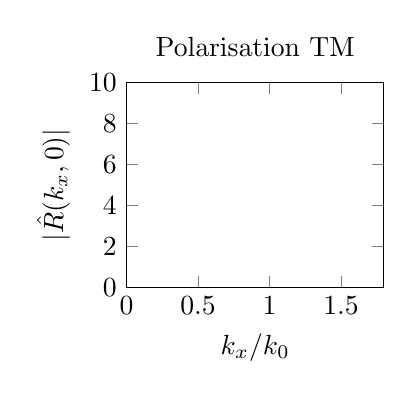
\begin{tikzpicture}[scale=1]
    \begin{axis}[
            title={Polarisation TM},
            ylabel={\(|\hat{R}(k_x,0)|\)},
            xlabel={\(k_x\slash k_0\)},
            width=0.4\textwidth,
            ymin=0,
            ymax=10,
            restrict y to domain=0:+4E+01,
            xmin=0,
            xmax=1.8,
            mark repeat=40,
            legend pos=outer north east
        ]
        % \addplot [color=black,mark=square*] table [col sep=comma, x={s1}, y={Abs(r_ex.11)}] {csv/SOUDAIS/SOUDAIS.r_ex.MODE_2_TYPE_P.csv};
        % % \addlegendentry{Exact};

        % \addplot [color=\ccio,mark=x] table [col sep=comma, x={s1}, y={Abs(r_ibc0.11)}] {csv/SOUDAIS/SOUDAIS.r_ibc.IBC_ibc0_SUC_F_MODE_2_TYPE_P.csv};
        % % \addlegendentry{CI0};

        % \addplot [color=\ccit,mark=diamond*] table [col sep=comma, x={s1}, y={Abs(r_ibc3.11)}] {csv/SOUDAIS/SOUDAIS.r_ibc.IBC_ibc3_SUC_F_MODE_2_TYPE_P.csv};
        % % \addlegendentry{CI3};
    \end{axis}
\end{tikzpicture}
\tikzsetnextfilename{R_SOUDAIS_plan_hoibc.TE}
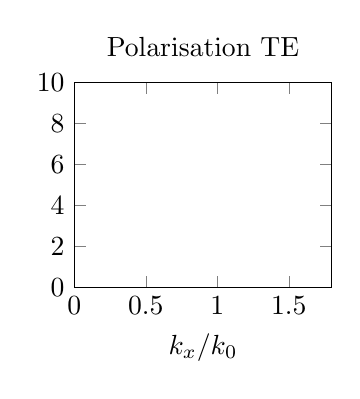
\begin{tikzpicture}[scale=1]
    \begin{axis}[
            title={Polarisation TE},
            ylabel={},
            xlabel={\(k_x\slash k_0\)},
            width=0.4\textwidth,
            xmin=0,
            xmax=1.8,
            ymin=0,
            ymax=10,
            mark repeat=40,
            legend pos=outer north east
        ]
        % \addplot [color=black,mark=square*] table [col sep=comma, x={s1}, y={Abs(r_ex.22)}] {csv/SOUDAIS/SOUDAIS.r_ex.MODE_2_TYPE_P.csv};
        % \addlegendentry{Exact};

        % \addplot [color=\ccio,mark=x] table [col sep=comma, x={s1}, y={Abs(r_ibc0.22)},color=] {csv/SOUDAIS/SOUDAIS.r_ibc.IBC_ibc0_SUC_F_MODE_2_TYPE_P.csv};
        % \addlegendentry{CI0};

        % \addplot [color=\ccit,mark=diamond*] table [col sep=comma, x={s1}, y={Abs(r_ibc3.22)}] {csv/SOUDAIS/SOUDAIS.r_ibc.IBC_ibc3_SUC_F_MODE_2_TYPE_P.csv};
        % \addlegendentry{CI3};
    \end{axis}
\end{tikzpicture}
      %     \caption[CIOE sur empilement de P.~Soudais p.~11]{Module des coefficients diagonaux de \(\mR\) pour \(\eps = 4, \mu = 1, d=0.035\text{m}, f=12\text{GHz}\)}
      %     \label{fig:reflex_fourier:plan:soudais:hoibc}
      % \end{figure}

      La figure \ref{fig:imp_fourier:plan:triple_asymptote:hoibc} montre la limite de la CI3 pour capturer trois asymptotes. Pour cela, il faudrait utiliser une CI d'ordre au moins 6 sur l'opérateur agissant sur \(\vE_t\). La CI3 n'est donc une bonne CIOE que si le nombre d'asymptotes est inférieur à 1, ce que l'on peut calculer connaissant l'empilement (voir proposition \ref{prop:imp_plan:symb_z:1c}).

      Si la matrice d'impédance exacte possède plusieurs asymptotes, il faut autant de pôles à la CIOE pour être une bonne approximation.

      L'expression d'une CIOE vérifiant ce critère est la \hyperlink{ci7}{CI7}
      \begin{equation}
        \left(\oI + \sum_{i=1}^3 \left(d_{i} \left(\frac{\LD}{k_0^2}\right)^i + e_{i} \left(-\frac{\LR}{k_0^2}\right)^i \right)\right)\vE_t = \left(a_0 \oI + \sum_{i=1}^3 \left(b_{i} \left(\frac{\LD}{k_0^2}\right)^i + c_{i} \left(-\frac{\LR}{k_0^2}^i\right) \right)\right)\vJ.
      \end{equation}

      \begin{figure}[!hbt]
          \centering
          \tikzsetnextfilename{Z_triple_asymptote_plan_hoibc.TM}
\begin{tikzpicture}[scale=1]
    \begin{axis}[
            title={Polarisation TM},
            ylabel={\(\Im(\hat{Z}(k_x,0)\)},
            xlabel={\(k_x\slash k_0\)},
            width=0.4\textwidth,
            xmin=0,
            xmax=1.999,
            ymin=-10,
            ymax=10,
            restrict y to domain=-300:300,
            mark repeat=200,
            legend pos=outer north east
        ]
        \addplot [color=black,mark=square*] table [col sep=comma, x={s1}, y={Im(z_ex.tm)}] {csv/triple_asymptote/triple_asymptote.z_ex.MODE_2_TYPE_P.csv};
        % \addlegendentry{Exact};

        \addplot [color=blue,mark=x] table [col sep=comma, x={s1}, y={Im(z_ibc0.tm)}] {csv/triple_asymptote/triple_asymptote.z_ibc.IBC_ibc0_SUC_F_MODE_2_TYPE_P.csv};
        % \addlegendentry{CI0};

        \addplot [color=red,mark=diamond*] table [col sep=comma, x={s1}, y={Im(z_ibc3.tm)}] {csv/triple_asymptote/triple_asymptote.z_ibc.IBC_ibc3_SUC_F_MODE_2_TYPE_P.csv};
        % \addlegendentry{CI3};

        \addplot [color=cyan,mark=pentagon*] table [col sep=comma, x={s1}, y={Im(z_ibc7.tm)}] {csv/triple_asymptote/triple_asymptote.z_ibc.IBC_ibc7_SUC_F_MODE_2_TYPE_P.csv};
        % \addlegendentry{CI7};
    \end{axis}
\end{tikzpicture}
\tikzsetnextfilename{Z_triple_asymptote_plan_hoibc.TE}
\begin{tikzpicture}[scale=1]
    \begin{axis}[
            title={Polarisation TE},
            ylabel={},
            xlabel={\(k_x\slash k_0\)},
            width=0.4\textwidth,
            xmin=0,
            xmax=1.999,
            ymin=-10,
            ymax=10,
            restrict y to domain=-300:300,
            mark repeat=200,
            legend pos=outer north east
        ]
        \addplot [color=black,mark=square*] table [col sep=comma, x={s1}, y={Im(z_ex.te)}] {csv/triple_asymptote/triple_asymptote.z_ex.MODE_2_TYPE_P.csv};
        \addlegendentry{Exact};

        \addplot [color=blue,mark=x] table [col sep=comma, x={s1}, y={Im(z_ibc0.te)}] {csv/triple_asymptote/triple_asymptote.z_ibc.IBC_ibc0_SUC_F_MODE_2_TYPE_P.csv};
        \addlegendentry{CI0};

        \addplot [color=red,mark=diamond*] table [col sep=comma, x={s1}, y={Im(z_ibc3.te)}] {csv/triple_asymptote/triple_asymptote.z_ibc.IBC_ibc3_SUC_F_MODE_2_TYPE_P.csv};
        \addlegendentry{CI3};

        \addplot [color=cyan,mark=pentagon*] table [col sep=comma, x={s1}, y={Im(z_ibc7.te)}] {csv/triple_asymptote/triple_asymptote.z_ibc.IBC_ibc7_SUC_F_MODE_2_TYPE_P.csv};
        \addlegendentry{CI7};                  
    \end{axis}
\end{tikzpicture}
          \caption[CIOE sur empilement avec triple asymptote]{Partie imaginaire des coefficients diagonaux de \(\mZ\) pour \(\eps = 4, \mu = 1, d=0.2\text{m}, f=1\text{GHz}\)}
          \label{fig:imp_fourier:plan:triple_asymptote:hoibc}
      \end{figure}
      \begin{table}[!hbt]
        \centering
        \begin{minipage}[t]{0.49\textwidth}
        \vspace{0pt}
        \centering
        \begin{coefftable}{\hyperlink{ci0}{CI0}}
          \input{csv/triple_asymptote/triple_asymptote.IBC_ibc0_SUC_F_MODE_2_TYPE_P.coeff.txt}
        \end{coefftable}

        \begin{coefftable}{\hyperlink{ci3}{CI3}}
          \input{csv/triple_asymptote/triple_asymptote.IBC_ibc3_SUC_F_MODE_2_TYPE_P.coeff.txt}
        \end{coefftable}
        \end{minipage}
        \tablecoeff[0.49]{\hyperlink{ci7}{CI7}}{csv/triple_asymptote/triple_asymptote.IBC_ibc7_SUC_F_MODE_2_TYPE_P.coeff.txt}
        \caption{Coefficients associés à la figure \ref{fig:imp_fourier:plan:triple_asymptote:hoibc}}
        \label{tab:imp_fourier:plan:triple_asymptote:hoibc}
      \end{table}

\subsection{Problème de la singularité de l'impédance dans le cadre du plan infini pour une couche de matériau sans perte}

Dans la thèse de \cite{aubakirov_electromagnetic_2014}, les constantes de la couche de matériau \(\eps=4,\mu=1,f=12\) GHz, et \(d=3.5\) mm. 
%Ce cas non physique possède un onde guidée pour \((k_x,k_y) = (k_0s^\star,0.)\) où \(\mR(k_0s^\star,0.) = \infty\).

Il existe un \(s_z\) tel que \(\hat\mZ_{ex}(k_0s_z,0.) = \infty\) si \(\eps\mu\in\RR\).
En effet, d'après la formule pour une couche de matériaux de la définition \ref{def:plan:impedance:1c}, 
% \begin{REM}
%   Dis dans le texte (et non seulement dans le titre) que ce n'est possible que si \(\eps\mu\in\RR\).
% \end{REM}
\begin{equation}
  \hat{\mZ}_{ex}(k_x,0.) = i\frac{\eta}{k\sqrt{k^2 - k_x^2}}\tan(\sqrt{k^2 - k_x^2}d)\left(k^2\mI - \hat{\mLR}\right).
\end{equation}
Ainsi, il est facile de voir que l'on a une asymptote à cause de la tangente, et donc pour cet empilement
\begin{equation}
  \label{eq:plan:asymptote_1_couche}
  s_z = \sqrt{\eps \mu - \left(\frac{\pi/2}{k_0 d}\right)^2}.
\end{equation}
% \begin{REM}[asymptote]
%   Et voilà l'explication de \hyperlink{REMnoasymptote}{la precedente remarque}.
% \end{REM}
Le problème est donc que si nous balayons en incidence et que l'on passe par ce point, alors la matrice \(\hat\mZ\) n'est pas définie en ce point.
Or comme le gradient de la fonction est fonction de cette matrice, le gradient n'est pas défini pour tout \(X\).
Si l'on utilise une méthode basée sur le gradient de type Newton, ce que nous avons fait, on comprend pourquoi la méthode numérique échoue à calculer des coefficients.

Dans le code numérique, la discrétisation en incidence et linéaire et nous passions par ce point.
En discrétisant différemment l'incidence, peut-être aurions-nous pu éviter cette difficulté.
\begin{REM}
et une autre méthode de minimisation
\end{REM} 
\begin{REP}
  Question à prévoir.
\end{REP}
\subsubsection{Réduction du nombre de variables de la minimisation}

On décompose alors nos matrices et vecteurs en séparant les parties contentant cette asymptote.

On suppose donc qu'il existe \({\mH}_\infty, {b}_\infty, X_\infty,\) tels que
\begin{align*}
  {\mH} &= {\mH}_\infty + {\mH}_r,
  \\
  {b} &= {b}_\infty + {b}_r,
  \\
  X &= X_\infty + X_r.
\end{align*}

Ces matrices et vecteurs sont reliés par les relations
\begin{align}
  {\mH}_\infty X_\infty &= {b}_\infty,
  \\
  {\mH}_\infty X_r &= 0.
\end{align}

Il faut voir cette décomposition comme deux parties, où l'une est nulle quasiment partout sauf pour le \(s_z\) problématique, et l'autre est définie normalement sauf aux termes correspondant au \(s_z\) où elle est nulle.

Schématiquement, on définit \(i_z\) l'indice d'une ligne telle que \({b}(\hat{\mZ})_{i_z} = \infty\), 

\begin{equation*}
  \begin{matrix}
    {\mH} &=& {\mH}_\infty &+& {\mH}_r,
    \\
    \begin{bmatrix}
      {\mH}_{1,1} & \cdots & {\mH}_{1,N_{CI}}
      \\
      \vdots & \ddots & \vdots
      \\
      {\mH}_{i_z-1,1} & \cdots & {\mH}_{i_z-1,N_{CI}}
      \\
      {\mH}_{i_z,1} & \cdots & {\mH}_{i_z,N_{CI}}
      \\
      {\mH}_{i_z+1,1} & \cdots & {\mH}_{i_z+1,N_{CI}}
      \\
      \vdots & \ddots & \vdots
      \\
      {\mH}_{4N_i,1} & \cdots & {\mH}_{4N_i,N_{CI}}
    \end{bmatrix}
    & = &
    \begin{bmatrix}
      0 & \cdots & 0
      \\
      \vdots & \ddots & \vdots
      \\
      0 & \cdots & 0
      \\
      {\mH}_{i_z,1} & \cdots & {\mH}_{i_z,N_{CI}}
      \\
      0 & \cdots & 0
      \\
      \vdots & \ddots & \vdots
      \\
      0 & \cdots & 0
    \end{bmatrix}
    & + & 
    \begin{bmatrix}
      {\mH}_{1,1} & \cdots & {\mH}_{1,N_{CI}}
      \\
      \vdots & \ddots & \vdots
      \\
      {\mH}_{i_z-1,1} & \cdots & {\mH}_{i_z-1,N_{CI}}
      \\
      0 & \cdots & 0
      \\
      {\mH}_{i_z+1,1} & \cdots & {\mH}_{i_z+1,N_{CI}}
      \\
      \vdots & \ddots & \vdots
      \\
      {\mH}_{4N_i,1} & \cdots & {\mH}_{4N_i,N_{CI}}
    \end{bmatrix}
  \end{matrix}.
\end{equation*}
Dans les faits, \({\mH}_\infty\) a \(4\) lignes non nulles et \({\mH}_r\) en a autant de nulles aux mêmes endroits.


On développe donc la fonction
% \begin{REM}
%   Voir \hyperlink{REMfonction}{avant}.
%   De plus, il est préférable de l'écrire sur le carré de la norme.
% \end{REM}
% \begin{REP}
%   Fait
% \end{REP}
suivant cette décomposition :
\begin{align*}
\argmin{X}\left\rVert {\mH} X - {b} \right \rVert^2 &= \argmin{X_r}\left\rVert \left({\mH}_\infty + {\mH}_r\right)\left( X_\infty + X_r \right) - {b}_\infty - {b}_r \right \rVert^2.
\\
\intertext{On utilise la relation entre \({\mH}_\infty X_\infty\) et \({b}_\infty\)}
&=  \argmin {X_r}\left\rVert {\mH}_\infty X_r + {\mH}_r X_\infty + {\mH}_r X_r - {b}_r \right \rVert^2.
\\
\intertext{Enfin par définition de \({\mH}_\infty\) et \(X_r\), leur produit est nul}
&= \argmin{X_r} \left\rVert {\mH}_r ( X_r + X_\infty)- {b}_r \right \rVert^2.
\end{align*}

On voit alors que l'on peut résoudre le problème
% \begin{REM}
%   Ce n'est pas rigoureux
% \end{REM}
% \begin{REP}
%   Pourtant c'est issus du travail à Montréal.
% \end{REP}
si l'on minimise uniquement sur les \(X_r\), les autres étant fixés, et si l'on enlève du système les lignes où l'impédance n'est pas définie.

\subsubsection{Application de la réduction à la CI3}

On rappelle l'expression de la CI3
\begin{equation*}
  \hat{\mZ}_{ap}(k_x,0) = \left(\mI + b_1 \hat{\mLD}(k_x,0) - b_2 \hat{\mLR}(k_x,0) \right)^{-1}\left(a_0\mI + a_1 \hat{\mLD}(k_x,0) - a_2 \hat{\mLR}(k_x,0) \right).
\end{equation*}

% On voit donc que pour faire apparaître une asymptote,
% \begin{REM}
%   Pas math. "Une condition nécessaire et suffisante pour que \(\mZ\) ai une asymptote est".
%   Elle est peut être seulement nécessaire car si \(a_0\mI + a_1\mLD -a_2\mLR\) a un noyau
% \end{REM}
% \begin{REP}
%   FAIT
% \end{REP}
Une condition nécessaire et suffisante pour que \(\hat{\mZ}_{ap}\) ait une asymptote est que la matrice de gauche ne soit pas inversible en \(s_z\).

La matrice \({\mH}_\infty\) est donc nulle partout sauf en 8 termes, placés sur les deux dernières colonnes et les 4 lignes correspondantes à \((k_x,k_y)=(k_0 s_z,0)\).

Connaissant les expressions des matrices \(\hat\mLD,\hat\mLR\) introduites dans la partie précédente alors on déduit que
\begin{align*}
  X_\infty = \begin{bmatrix}
    0\\
    0\\
    0\\
    (k_0 s_z)^{-2}\\
    (k_0 s_z)^{-2}\\
  \end{bmatrix},
  & &
  X_r = \begin{bmatrix}
  a_0\\
  a_1\\
  a_2\\
  0\\
  0\\
  \end{bmatrix}.
\end{align*}

\subsection{Choix de la méthode numérique pour résoudre la minimisation sous contraintes}

  Des méthodes basées sur le gradient sont adaptées, car la fonction est dérivable pour tout \(X\) et les contraintes se comportent comme des polynômes dépendant uniquement des composantes de \(X\). Nous avons donc fait le choix de la méthode \gls{acr-sqp} pour les raisons suivantes:
 
  \begin{itemize}
    \item elle est éprouvée depuis \cite{kraft_software_1988} et des sources Fortran à jour sont disponibles à \url{https://github.com/jacobwilliams/slsqp}, ce qui est capital pour l'intégrer dans un code industriel ;
    \item elle est rapide, nous avons observé que cette méthode convergeait en quelques dizaines d'itérations au plus ;
    \item elle accepte des contraintes non linéaires, donc elle est adaptée à nos CSU.
  \end{itemize}

% \subsection{Résultats numérique avec contraintes}

  % \begin{REM}
  %   Quelques résultats avec contraintes
  % \end{REM}

\section{Calcul des coefficients de la CI3 par moindres carrés sur les coefficients de la série de Fourier}

  On peut aussi résoudre calculer les coefficients en minimisant l'erreur entre les coefficients de Fourier.

  Soit \(\mM_A\) et \(\mM_B\) les fonctions introduites à la définition \ref{def:plan:matrices_MA-MB} et \(\hat\mR\) la fonction définie en \ref{def:plan:reflexion:impedance}.

  \begin{defn}%[]
    \label{def:plan:minimisation:matrices_MR}
    On définit les fonctions \(\hat\mR_{ex}, \hat\mR_{CI3}\) de \(\RR\times\RR\times \rightarrow \mathcal{M}_2(\CC)\) telles que
    \begin{align*}
      \hat\mR_{ex}(k_x,k_y) &= \hat\mR(k_x,k_y, \hat\mZ_{ex}(k_x,k_y))
      \\
      \hat\mR_{CI3}(k_x,k_y) &= \hat\mR(k_x,k_y, \hat\mZ_{CI3}(k_x,k_y))
    \end{align*}
    où \(\hat\mZ_{ex},\hat\mZ_{CI3}\) sont des fonctions définies à la proposition \ref{prop:plan:synthese:impedance} et à l'équation \eqref{eq:plan:hoibc:ci3}.
  \end{defn}

  \subsection[Expression de la fonctionnelle JR]{Expression de la fonctionnelle \(J_R\)}

    On utilise les fonctions \(\mN_E, \mN_H\) introduites à la définition \ref{def:plan:matrices_NE-NH} et \(\hat\mLD,\hat\mLR\) définies aux définitions \ref{eq:plan:fourier:LD}-\ref{eq:plan:fourier:LR}.

    \begin{defn}
      On définit \(\mA_0,\mA_1,\mA_2,\mA_2,\mB_1,\mB_2\) les fonctions de \(\RR \times \RR \times \mathcal{M}_2(\CC) \rightarrow \ \mathcal{M}_2(\CC)\) telles que        
      \begin{align*}
        \mA_0(k_x,k_y,\mR) &= \mN_E(k_x,k_y,0^+,\mR)
        \\
        \mA_1(k_x,k_y,\mR) &= \hat{\mLD}(k_x,k_y)\mN_E(k_x,k_y,0^+,\mR)
        \\
        \mA_2(k_x,k_y,\mR) &= -\hat{\mLR}(k_x,k_y)\mN_E(k_x,k_y,0^+,\mR)
        \\
        \mB_1(k_x,k_y,\mR) &= \hat{\mLD}(k_x,k_y)\mN_H(k_x,k_y,0^+,\mR)
        \\
        \mB_2(k_x,k_y,\mR) &= -\hat{\mLR}(k_x,k_y)\mN_H(k_x,k_y,0^+,\mR)            
      \end{align*}

      On définit \(\tilde{\mH}_{CI3}\) la fonction de \(\RR \times \RR \times \mathcal{M}_2(\CC) \rightarrow \mathcal{M}_{4\times5}(\CC)\) telle que
      \begin{align*}
        & \tilde\mH_{CI3}(k_x,k_y,\mR) =  \\ &
        \begin{bmatrix}
          \mA_0(k_x,k_y,\mR)_{11} & \mA_1(k_x,k_y,\mR)_{11} & \mA_2(k_x,k_y,\mR)_{11} & \mB_1(k_x,k_y,\mR)_{11} & \mB_2(k_x,k_y,\mR)_{11}
          \\
          \mA_0(k_x,k_y,\mR)_{12} & \mA_1(k_x,k_y,\mR)_{12} & \mA_2(k_x,k_y,\mR)_{12} & \mB_1(k_x,k_y,\mR)_{12} & \mB_2(k_x,k_y,\mR)_{12}
          \\
          \mA_0(k_x,k_y,\mR)_{21} & \mA_1(k_x,k_y,\mR)_{21} & \mA_2(k_x,k_y,\mR)_{21} & \mB_1(k_x,k_y,\mR)_{21} & \mB_2(k_x,k_y,\mR)_{21}
          \\
          \mA_0(k_x,k_y,\mR)_{22} & \mA_1(k_x,k_y,\mR)_{22} & \mA_2(k_x,k_y,\mR)_{22} & \mB_1(k_x,k_y,\mR)_{22} & \mB_2(k_x,k_y,\mR)_{22}
        \end{bmatrix}
      \end{align*}

      On définit \(\tilde{b}\) la fonction de \(\RR \times \RR \times \mathcal{M}_2(\CC) \rightarrow \mathcal{M}_{4\times1}(\CC)\) telle que
      \begin{equation*}
        \tilde{b}(k_x,k_y,\mR) = -
        \begin{bmatrix}
          \mN_H(k_x,k_y,0^+,\mR)_{11}
          \\
          \mN_H(k_x,k_y,0^+,\mR)_{12}
          \\
          \mN_H(k_x,k_y,0^+,\mR)_{21}
          \\
          \mN_H(k_x,k_y,0^+,\mR)_{22}
        \end{bmatrix}
      \end{equation*}
    \end{defn}

    \begin{prop}
      Soit \(X = (a_0,a_1,a_2,b_1,b_2)\), \((k_x,k_y)\) fixé et \(\hat\mR_{ex}\) la matrice définie en \ref{def:plan:minimisation:matrices_MR}, alors
      \begin{multline*}
        \argmin{X\in\CC^5} \norm{\hat\mR_{CI3}(k_x,k_y,X) - \hat\mR_{ex}(k_x,k_y)} =
        \\
        \argmin{X\in\CC^5} \norm{\tilde{\mH}_{CI3}(k_x,k_y,\hat\mR_{ex}(k_x,k_y))X - \tilde{b}(k_x,k_y,\hat\mR_{ex}(k_x,k_y))}
      \end{multline*}
    \end{prop}

    \begin{proof}
      C'est la même méthodologie que pour l'impédance.
      On rappelle de la section précédente
      \begin{multline*}
        \hat{\mZ}_{CI3}(k_x,k_y) = \left(\mI + b_1 \hat{\mLD}(k_x,k_y) - b_2 \hat{\mLR}(k_x,k_y) \right)^{-1}
        \\
        \left(a_0 \mI + a_1 {\hat{\mLD}(k_x,k_y)} - a_2 {\hat{\mLR}(k_x,k_y)}\right)
      \end{multline*}
      On pose \(\hat\mZ_D(k_x,k_y) = \mI + b_1 \hat{\mLD}(k_x,k_y) - b_2 \hat{\mLR}(k_x,k_y)\) et \(\hat\mZ_N(k_x,k_y) = a_0 \mI + a_1 {\hat{\mLD}(k_x,k_y)} - a_2 {\hat{\mLR}(k_x,k_y)}\) donc

      \begin{align*}
        &{\hspace{1em}}~ \argmin{X\in\CC^5} \norm{\hat\mR_{CI3}(k_x,k_y,X) - \hat\mR_{ex}(k_x,k_y)}
        \\
        & = \argmin{X\in\CC^5} \norm{ - \mM_B(k_x,k_y,0^+,\hat\mZ_{CI3})^{-1}\mM_A(k_x,k_y,0^+,\hat\mZ_{CI3})- \hat\mR_{ex}(k_x,k_y) }
        \\
        & = \argmin{X\in\CC^5} \norm{ - \mM_B(k_x,k_y,0^+,\hat\mZ_{CI3})^{-1}\left(\mM_A(k_x,k_y,0^+,\hat\mZ_{CI3}) +  \mM_B(k_x,k_y,0^+,\hat\mZ_{CI3})\hat\mR_{ex}(k_x,k_y)\right) }      
        \\ 
        & = \argmin{X\in\CC^5} \norm{\mM_A(k_x,k_y,0^+,\hat\mZ_{CI3}) +\mM_B(k_x,k_y,0^+,\hat\mZ_{CI3})\hat\mR_{ex}(k_x,k_y)}
        \intertext{D'après la définition \ref{def:plan:matrices_MA-MB} des fonctions \(\mM_A, \mM_B\),}
        & = \argmin{X\in\CC^5} \left\lVert \left(\mJ_E(k_x,k_y,0^+)-\hat\mZ_{CI3}(k_x,k_y)\mJ_H(k_x,k_y,0^+)\right) \right.
        \\
        & \qquad \qquad \quad + \left.\left(\mH_E(k_x,k_y,0^+)-\hat\mZ_{CI3}(k_x,k_y)\mH_H(k_x,k_y,0^+)\right)\hat\mR_{ex}(k_x,k_y) \right\lVert
        \intertext{D'après la définition de \(\hat\mZ_{CI3}\),}        
        & = \argmin{X\in\CC^5} \left\lVert \hat\mZ_D(k_x,k_y)^{-1}\left(\hat\mZ_D(k_x,k_y)\mJ_E(k_x,k_y,0^+)-\hat\mZ_N(k_x,k_y)\mJ_H(k_x,k_y,0^+)\right) \right.
        \\
        & \qquad \qquad \quad + \left.\hat\mZ_D(k_x,k_y)^{-1}\left(\hat\mZ_D(k_x,k_y)\mH_E(k_x,k_y,0^+)-\hat\mZ_N(k_x,k_y)\mH_H(k_x,k_y,0^+)\right)\hat\mR_{ex}(k_x,k_y) \right\lVert
        \\
        & = \argmin{X\in\CC^5} \left\lVert \left(\hat\mZ_D(k_x,k_y)\mJ_E(k_x,k_y,0^+)-\hat\mZ_N(k_x,k_y)\mJ_H(k_x,k_y,0^+)\right) \right.
        \\
        & \qquad \qquad \quad + \left.\left(\hat\mZ_D(k_x,k_y)\mH_E(k_x,k_y,0^+)-\hat\mZ_N(k_x,k_y)\mH_H(k_x,k_y,0^+)\right)\hat\mR_{ex}(k_x,k_y) \right\lVert
        \intertext{D'après la définition \ref{def:plan:matrices_NE-NH} des fonctions \(\mN_E, \mN_H\),}        
        & = \argmin{X\in\CC^5} \norm{\hat\mZ_N(k_x,k_y)\mN_E(k_x,k_y,0^+,\hat\mR_{ex}(k_x,k_y)) + \hat\mZ_D(k_x,k_y)\mN_H(k_x,k_y,0^+,\hat\mR_{ex}(k_x,k_y))}
      \end{align*}
      et l’on conclut d'après la définition des fonctions \(\hat\mZ_D, \hat\mZ_N\).
    \end{proof}

    \begin{defn}
      On définit \(\tilde{\mA}_{CI3}\) la matrice de \(\mathcal{M}_{4N_{n}N_{k_z}\times5}(\CC)\) telle que
      \begin{equation*}
        \tilde{\mA}_{CI3} = 
        \begin{bmatrix}
          \tilde\mH_{CI3}(n_1,k_{z1},\hat\mR_{ex}(n_1,k_{z1}))
          \\
          \vdots
          \\
          \tilde\mH_{CI3}(n_i,k_{zj},\hat\mR_{ex}(n_i,k_{zj}))
          \\
          \vdots
          \\
          \tilde\mH_{CI3}(n_{N_n},k_{zN_{k_z}},\hat\mR_{ex}(n_{N_n},k_{zN_{k_z}}))
        \end{bmatrix}
      \end{equation*}
      On définit \(\tilde{g}\) le vecteur colonne \(\CC^{4N_{n}N_{k_z}}\) telle que
      \begin{equation*}
        \tilde{g} = 
        \begin{bmatrix}
          \tilde{b}(n_1,k_{z1},\hat\mR_{ex}(n_1,k_{z1}))
          \\
          \vdots
          \\
          \tilde{b}(n_i,k_{zj},\hat\mR_{ex}(n_i,k_{zj}))
          \\
          \vdots
          \\
          \tilde{b}(n_{N_n},k_{zN_{k_z}},\hat\mR_{ex}(n_{N_n},k_{zN_{k_z}}))
        \end{bmatrix}
      \end{equation*}
    \end{defn}

    On peut alors calculer les coefficients de la CI3

    \begin{defn}
      On définit la fonctionnelle \(J_R\)
      \begin{equation*}
        J_R(X) = \norm{\tilde{\mA}_{CI3}X - \tilde{g}}
      \end{equation*}
    \end{defn}

    \begin{thm}[Minimisation sans contraintes pour la CI3]

      Les coefficients de la CIOE sont solutions du problème

      Trouver \(X^* \in \CC^5\) tel que
      \begin{equation*}
        X^* = \argmin{X\in \CC^5} J_R(X)
      \end{equation*}
    \end{thm}

    \begin{prop}
      Si \(\conj{\tilde{\mA}_{CI3}^t}\tilde{\mA}_{CI3}\) est inversible alors
      \begin{equation*}
        X^* = (\conj{\tilde{\mA}_{CI3}^t}\tilde{\mA}_{CI3})^{-1}\conj{\tilde{\mA}_{CI3}^t}\tilde{g}
      \end{equation*}
    \end{prop}
    \begin{proof}
      Même méthode que pour la proposition \ref{prop:plan:minimisation:minimum_sans_contraintes} sur l'impédance.
    \end{proof}

    Nous n'avons pas réussi à démontrer que cette matrice était définie pour tout empilement et toute incidence, pas même pour des CIOE plus simples.

    \begin{thm}[Minimisation avec contraintes pour la CI3]

      Soit \(\CSU[3]{CI3}\) le sous-espace de \(\CC^5\) issu de la définition \ref{def:csu:ci3-3}.
      Alors les coefficients de la CIOE respectant les CSU sont solutions du problème

      Trouver \(X^* \in \CC^5\) tel que
      \begin{equation*}
        X^* = \argmin{X\in \CSU[3]{CI3}} J_R(X)
      \end{equation*}
    \end{thm}

    


\sectionstar{Conclusion}
Nous avons montré comment calculer les coefficients dans le cas d'un objet plan infini plan en minimisant au sens des moindres carrés la différence entre les matrices d'impédance exactes et approchées. 

Pour cela, nous avons réalisé une analyse spectrale des équations de Maxwell et montré que la condition d'impédance s'exprime comme un multiplicateur de Fourier matriciel, tout comme la matrice de réflexion. Grâce à cette analyse spectrale, nous avons aussi exprimé les CIOE comme des multiplicateurs de Fourier matriciels dont on a déduit la matrice de réflexion associée. Nous avons alors exprimé le problème de minimisation sous contraintes et montré que celui-ci a besoin d'être réduit dans le cas d'une couche de matériau sans pertes.

Nous avons alors conclu que la \hyperlink{ci3}{CI3} était la plus performante et que le jeu de CSU retenu dans la partie précédente permettait d'obtenir de bons coefficients de réflexions.

        \chapter{Calcul des coefficients pour un cylindre infini}
\label{sec:cylindre}
\minitoc
\newpage
\sectionstar{Introduction}
L'introduction de courbures dans les CIOE est un atout majeur, car les objets réels sont rarement plats, mais plutôt de type cylindre ou sphère-cone. Nous présentons dans cette partie le cas d'un cylindre infini.

\section{Expressions exactes des matrices d'impédance et des matrice de réflexions pour un cylindre infini}

  % On rappelle les formules des opérateurs \(\vdiv, \vrot\) en coordonnée cylindrique \((r,\theta,z)\).
  % \begin{align}
  %   \vrot \vect{V} &= \left(\frac{1}{r}\ddr{\theta}{V_z} - \ddr{z}{V_\theta}\right)\vect{e_r} +
  %   \left(\ddr{z}{V_r} - \ddr{r}{V_z}\right)\vect{e_\theta} +
  %   \frac{1}{r}\left(\ddr{r}{(rV_\theta)}-\ddr{\theta}{V_r}\right)\vect{e_z}
  %   \\
  %   \vdiv \vect{V} &= \frac{1}{r}\ddr{r}{(rV_r)}+\frac{1}{r}\ddr{\theta}{V_\theta}+\ddr{z}{V_z}
  %   \\
  %   \vgrad f &= \ddr{r}{f}\vect{e_r}
  %   +\frac{1}{r}\ddr{\theta}{f}\vect{e_\theta} + \ddr{z}{f}\vect{e_z}
  % \end{align}

  \begin{figure}[!hbt]
    \centering
    \tikzsetnextfilename{cylindre_1_couche}
    \begin{tikzpicture}
      \coordinate (mat) at (0,-1.5);
\coordinate (vide) at (0,-2);
\coordinate (c) at (0,0);

\fill [lightgray] (c) circle (2);
\fill [white] (c) circle (1.5);
\fill [pattern=north east lines] (c) circle (1.5);

\draw (c) circle (2);
\draw (c) circle (1.5);


\coordinate (n) at (0,2);

%\draw (vide) node [below] {$\eps_0,\mu_0$};
\draw (mat) node [below] {$\peps,\pmu$};

% Axess
\draw [->] (n) -- ++(0,1) node [at end, right] {$\v{\mr}$};
\draw [->] (n) -- ++(1,0) node [at end, right] {$\v{\mt}$};

\draw (n) ++(0.2,0.2) circle(0.1cm) node [above=0.1cm] {$\v{\mz}$};
\draw (n) ++(0.2,0.2) +(135:0.1cm) -- +(315:0.1cm);
\draw (n) ++(0.2,0.2) +(45:0.1cm) -- +(225:0.1cm);

%\draw [->>,thick] (lt) ++ (1,1) -- (mt) ;


    \end{tikzpicture}
  \end{figure}

  On exprime les équations de Maxwell dans le matériau dans la base cylindrique et sans pertes de généralité, on peut réaliser une transformée de Fourier en \(z\) par invariance en translation et en \(\theta\) par invariance en rotation.
  Cependant, le multiplicateur de Fourier associé à la coordonnée \(\theta\) doit être un entier pour assurer la périodicité. On le note \(n\). On n'a plus une transformée de Fourier mais une série de Fourier en \(\theta\) et une transformée de Fourier en \(z\).

  \begin{equation}
    \vE(r,\theta,z) = \frac{1}{2\pi}\sum_{n=-\infty}^{\infty}\int_{\RR} e^{i(n \theta + k_z z )}\hat{\vE} (r,n,k_z) \dd{k_z}
  \end{equation}

  Nous reprenons la méthode du plan infini en n'étudiant que \(\hat{\vE} (r,n,k_z)\) pour simplifier les équations différentielles.

  \begin{prop}
    Soit
    \begin{equation}
      k_3 = \sqrt{\w^2\eps\mu - k_z^2}
    \end{equation}
    et \(J_n(z)\) et \(H_n^{(2)}(z)\) des solutions de l'équation de Bessel d'ordre \(n\).

    Alors \(\exists (c_i(n,k_z))_{1\le i\le 4} \in \CC(\NN\times\RR)^4\) tels que
    \begin{subequations}
      \begin{align}
        \hat{E_z}(r,n,k_z) &= c_1(n,k_z) J_n\left(k_3r\right) + c_2(n,k_z) H_n^{(2)}\left(k_3r\right)
        \\
        \hat{H_z}(r,n,k_z) &= c_3(n,k_z) J_n\left(k_3r\right) + c_4(n,k_z) H_n^{(2)}\left(k_3r\right)
      \end{align}
    \end{subequations}
  \end{prop}

  \begin{proof}

    On peut simplifier les opérateurs différentiels:

    \begin{align}
      \vrot \hat \vE(r,n,k_z) &= i\left(\frac{n}{r}\hat{E_z} - k_z\hat{E_\theta}\right)\vect{e_r} +
      \left(ik_z\hat{E_r} - \ddr{r}{\hat{E_z}}\right)\vect{e_\theta} +
      \frac{1}{r}\left(\ddr{r}{(r\hat{E_\theta})}-in\hat{E_r}\right)\vect{e_z}
      \\
      &=-i\w\mu \hat \vH(r,n,k_z)
    \end{align}

    % On remarque que la méthode utilisée pour le plan aboutie à une équation différentielle à coefficients non constants de type \(r\ddr{r}{\vect{X}}(r,n,k_z) = \mat{M}(r,n,k_z)\vect{X}(r,n,k_z)\).
    % On ne peut pas exprimer la solution avec les valeurs et vecteurs propres de la matrice.
    %Nous allons donc trouver une équation de Bessel en développant le système de Maxwell.

    Comme l'on cherche \(\hat \vE_t, \hat \vH_t\), on remarque que les 2\ieme composantes des équations de Maxwell permettent de déduire \(\hat\vE_t, \hat\vH_t\) de \( \hat E_z, \hat H_z\). Il faut donc trouver une EDP dont ces deux quantités sont solution.

    On couple les 2 équations du système de Maxwell pour aboutir à une équation sur \(\hat \vE\) seul:

    % \begin{align}
    %   \vrot \vrot \hat \vE &= \w^2\eps\mu \hat \vE
    %   \\
    %   \vdiv \hat \vE &= 0
    % \end{align}

    % \begin{multline}
    %   \vrot \vrot \hat \vE = \dots\\
    %   i\left(\frac{n}{r^2}\left(\ddr{r}{(r\hat{E_\theta})} - in\hat{E_r}\right) - k_z\left(ik_z\hat{E_r} - \ddr{r}{\hat{E_z}}\right)\right)  \vect{e_r} \dots\\
    %   + \left(-k_z\left(\frac{n}{r}\hat{E_z} - k_z\hat{E_\theta}\right) -\ddr{r}{}\left(\frac{1}{r}\left(\ddr{r}{(r\hat{E_\theta})}-in\hat{E_r}\right)\right)\right)  \vect{e_\theta} \dots\\
    %   + \frac{1}{r}\left(\ddr{r}{} \left(r\left(ik_z\hat{E_r} - \ddr{r}{\hat{E_z}}\right)\right) + n \left(\frac{n}{r}\hat{E_z} - k_z\hat{E_\theta}\right)\right) \vect{e_z}
    % \end{multline}

    % On aboutit au système suivant
    \begin{equation}
      \left\lbrace
      \begin{array}{ccc}
        -\left(\w^2\eps\mu -\frac{n^2}{r^2}  - k_z^2\right)\hat{E_r}  +i\frac{n}{r^2}\ddr{r}{(r\hat{E_\theta})}  +k_z\ddr{r}{\hat{E_z}} & = & 0\\
        in\ddr{r}{}\left(\frac{\hat{E_r}}{r}\right) -\left(\w^2\eps\mu - k_z^2\right)\hat{E_\theta} + \ddr{r}{}\left(\frac{1}{r}\ddr{r}{(r\hat{E_\theta})}\right)  - n\frac{k_z}{r}\hat{E_z} & = & 0\\
        i\frac{k_z}{r}\ddr{r}{(r\hat{E_r})}  - n\frac{k_z}{r}\hat{E_\theta}  -\left(\w^2\eps\mu - \frac{n^2}{r^2} \right)\hat{E_z} - \frac{1}{r}\ddr{r}{}\left(r\ddr{r}{\hat{E_z}}\right) & = & 0
      \end{array}
      \right.
    \end{equation}

    De la troisième  équation, on trouve pour \(r\not=0\)
    \begin{equation}
    r^2 \ddr[2]{r}{\hat{E_z}} + r\ddr{r}{\hat{E_z}} + \left(r^2\w^2\eps\mu - n^2\right)\hat{E_z} =ik_zr\ddr{r}{(r\hat{E_r})} -  nk_zr\hat{E_\theta}
    \end{equation}

    Or comme par définition des équations de Maxwell, \(\vdiv \hat \vE = 0\), on a
    \begin{align}
      \vdiv\hat \vE &= \frac{1}{r}\ddr{r}{(r\hat{E_r})} + \frac{in}{r}\hat{E_\theta} + ik_z\hat{E_z}
      \\
      k_z^2r^2 \hat{E_z} &= ik_zr\ddr{r}{(r\hat{E_r})} - nk_zr\hat{E_\theta}
    \end{align}

    On obtient donc sur la composante \(\hat{E_z}\):
    \begin{equation}
      r^2 \ddr[2]{r}{\hat{E_z}} + r\ddr{r}{\hat{E_z}} + \left(r^2\left(\w^2\eps\mu - k_z^2\right) - n^2\right)\hat{E_z} = 0
    \end{equation}

    Si \(k_3^2 = k^2 - k_z^2\) est non-nul, c'est une équation de Bessel (cf \cite[eq (6.80)]{bowman_introduction_1958}),%\footnote{Sinon c'est une équation de Euler-Cauchy et les solutions sont de types \(c_1(n) \cosh(n\ln(r)) + c_2(n) i\sinh(n\ln(r))\)}
    dont des solutions générales sont: 

    Soient \((c_1(n,k_z),c_2(n,k_z)) \in \CC(\NN\times\RR)^2\):
    \begin{equation}
      \hat{E_z}(r,n,k_z) = c_1(n,k_z) J_n\left(k_3r\right) + c_2(n,k_z) H_n^{(2)}\left(k_3r\right)
    \end{equation}
    où \(J_n\) est la fonction de Bessel du premier type, \(H_n^{(2)}\) la fonction de Hankel de deuxième type.
    On sait que l'on peut prendre n'importe quel couple de fonctions de Bessel (cf \eqref{eq:annex:bessel:equiv_bessel}), on choisit ce dernier car les \(J_n\) sont régulières et les \(H_n\) évoluent en \(r^{-1 \slash 2}\) à l'infini, donc ce choix est adapté à une décomposition en une onde incidente partout définie et une onde réfléchie décroissante à l'infini.

    De plus, d'après \cite[p.~358]{abramowitz_handbook_1964}, on sait qu'une fonction de Bessel d'ordre \(n\) est linéairement dépendante de celle d'ordre \(-n\).
    On peut donc se restreindre à \(n\) entier naturel.

    On trouve exactement le même résultat pour \(\hat{H_z}\): 

    Soient \((c_3(n,k_z,c_4(n,k_z)) \in \CC(\NN\times\RR)^2\)
    \begin{equation}
      \hat{H_z}(r,n,k_z) = c_3(n,k_z) J_n\left(k_3r\right) + c_4(n,k_z) H_n^{(2)}\left(k_3r\right)
    \end{equation}
  \end{proof}


  \begin{defn}
    On définit les matrices \(\mJ_{E}(r,n,k_z),\mH_{E}(r,n,k_z),\mJ_{H}(r,n,k_z),\mH_{H}(r,n,k_z)\)
    \begin{align}
      \mJ_{E}(r,n,k_z) &=
      \begin{bmatrix}
        -\frac{nk_z}{rk_3^2}J_n(k_3r) & \frac{ik\eta}{k_3}J_n'(k_3r)
        \\
        J_n(k_3r) & 0
      \end{bmatrix}
      \\
      \mH_{E}(r,n,k_z) &=
      \begin{bmatrix}
        -\frac{nk_z}{rk_3^2}H_n^{(2)}(k_3r) & \frac{ik\eta}{k_3}H_n^{(2)}{}'(k_3r)
        \\
        H_n^{(2)}(k_3r) & 0
      \end{bmatrix}
      \\
      \mJ_{H}(r,n,k_z) &=
      \begin{bmatrix}
        0 & -J_n(k_3r)
        \\
        -\frac{ik}{\eta k_3}J_n'(k_3r) & -\frac{nk_z}{rk_3^2}J_n(k_3r)
      \end{bmatrix}
      \\
      \mH_{H}(r,n,k_z) &=
      \begin{bmatrix}
        0 & -H_n^{(2)}(k_3r)
        \\
        -\frac{ik}{\eta k_3}H_n^{(2)}{}'(k_3r) & -\frac{nk_z}{rk_3^2}H_n^{(2)}(k_3r)
      \end{bmatrix}
    \end{align}
  \end{defn}

  \begin{prop}
    Alors dans une couche, les champs tangentiels s'écrivent
    \begin{subequations}
      \begin{align}
        \hat \vE_t(r,n,k_z) &= \mJ_{E}(r,n,k_z)
        \begin{bmatrix}
          c_1(n,k_z) \\
          c_3(n,k_z)
        \end{bmatrix}
        +
        \mH_{E}(r,n,k_z)
        \begin{bmatrix}
          c_2(n,k_z) \\
          c_4(n,k_z)
        \end{bmatrix}
        \label{eq:imp_fourier:cylindre:Et}\\
        \vect{e_r}\times\hat \vH_t(r,n,k_z) &=
        \mJ_{H}(r,n,k_z)
        \begin{bmatrix}
          c_1(n,k_z) \\
          c_3(n,k_z)
        \end{bmatrix}
        +
        \mH_{H}(r,n,k_z)
        \begin{bmatrix}
          c_2(n,k_z) \\
          c_4(n,k_z)
        \end{bmatrix}
        \label{eq:imp_fourier:cylindre:Ht}
      \end{align}
    \end{subequations}
  \end{prop}


  \begin{proof}
    À partir des équations de Maxwell restantes, on peut déterminer \(\hat{E_r},\hat{E_\theta},\hat{H_r},\hat{H_\theta}\).
    \begin{equation}
      \left\lbrace
      \begin{matrix}
        -ik_z\hat{E_\theta} + i\w\mu \hat{H_r} = -\frac{in}{r}\hat{E_z}
        \\
        ik_z\hat{E_r} + i\w\mu \hat{H_\theta} = \ddr{r}{\hat{E_z}}
        \\
        i\w\eps \hat{E_r} + ik_z \hat{H_\theta} = \frac{in}{r}\hat{H_z}
        \\
        i\w\eps \hat{E_\theta} - ik_z \hat{H_r} = -\ddr{r}{\hat{H_z}}
      \end{matrix}
      \right.
    \end{equation}

    Cela revient à résoudre \(\vect{Y} = \mat{M}\vect{X}\) où la matrice \(\mat{M}\) et les vecteurs \(\vect{X}, \vect{Y}\) sont définis tels que
    \begin{equation}
      \mat{M} =
      \begin{bmatrix}
      0 & -ik_z & i\w\mu & 0
      \\
      ik_z & 0 & 0 & i\w\mu
      \\
      i\w\eps & 0 & 0 & ik_z
      \\
      0 & i\w\eps & -ik_z & 0
      \end{bmatrix}
      \,
      \vect{X} =
      \begin{bmatrix}
        \hat{E_r}\\
        \hat{E_\theta}\\
        \hat{H_r}\\
        \hat{H_\theta}
      \end{bmatrix}
      \,
      \vect{Y} =
      \begin{bmatrix}
        -\frac{in}{r}\hat{E_z}\\
        \ddr{r}{\hat{E_z}}\\
        \frac{in}{r}\hat{H_z}\\
        -\ddr{r}{\hat{H_z}}
      \end{bmatrix}
    \end{equation}

    On remarque que \(\mM\mM = \left(k_z^2 - \omega^2\eps\mu\right)\mI\) et donc que \(\det(\mat{M}) = ik_3\).

    % \subsection{Cas \(k_3\not=0\)}

    On suppose ce dernier non nul, on peut déduire \(\vect{X}\):

    \begin{equation}
      \begin{bmatrix}
        \hat{E_r}\\
        \hat{E_\theta}\\
        \hat{H_r}\\
        \hat{H_\theta}
      \end{bmatrix} =
      \frac{1}{-k_3^2}
      \begin{bmatrix}
      0 & -ik_z & i\w\mu & 0
      \\
      ik_z & 0 & 0 & i\w\mu
      \\
      i\w\eps & 0 & 0 & ik_z
      \\
      0 & i\w\eps & -ik_z & 0
      \end{bmatrix}
      \begin{bmatrix}
        -\frac{in}{r}\hat{E_z}\\
        \ddr{r}{\hat{E_z}}\\
        \frac{in}{r}\hat{H_z}\\
        -\ddr{r}{\hat{H_z}}
      \end{bmatrix}
    \end{equation}

    On extrait alors \(\hat{E_\theta}, \hat{H_\theta}\) pour obtenir les champs tangentielles à \(\vect{e_r}\) en tout point, sachant déjà \(\hat{E_z}, \hat{H_z}\).

    \begin{align}
      \hat{E_r} & = \frac{1}{k_3^2}\left(ik_z\ddr{r}{\hat{E_z}}+\frac{k\eta n}{r}\hat{H_z}\right)
      \\
      \hat{E_\theta} &= -\frac{1}{k_3^2}\left(\frac{nk_z}{r}\hat{E_z} - i\w\mu\ddr{r}{\hat{H_z}}\right)
      \\
      \hat{E_z} &= c_1 J_n(k_3 r) + c_2 H_n^{(2)}(k_3 r)
      \\
      -\hat{H_z} &= -c_3 J_n(k_3 r) - c_4 H_n^{(2)}(k_3 r)
      \\
      \hat{H_\theta} &= -\frac{1}{k_3^2}\left(i\w\eps\ddr{r}{\hat{E_z}} + \frac{nk_z}{r}\hat{H_z}\right)
    \end{align}

    On dérive les fonctions de Bessel:

     \begin{align}
      \hat{E_\theta} &= -\frac{nk_z}{rk_3^2}\left(c_1J_n(k_3r) + c_2 H_n^{(2)}(k_3r)\right) + \frac{ik\eta}{k_3}\left(c_3J_n'(k_3r) + c_4 H_n^{(2)}{}'(k_3r)\right)
      \\
      \hat{E_z} &= c_1 J_n(k_3 r) + c_2 H_n^{(2)}(k_3 r)
      \\
      -\hat{H_z} &= -c_3 J_n(k_3 r) - c_4 H_n^{(2)}(k_3 r)
      \\
      \hat{H_\theta} &= -\frac{ik}{\eta k_3}\left(c_1J_n'(k_3r) + c_2 H_n^{(2)}{}'(k_3r)\right) - \frac{nk_z}{rk_3^2}\left(c_3J_n(k_3r) + c_4 H_n^{(2)}(k_3r)\right)
    \end{align}

    Et on obtient

    \begin{subequations}
      \label{eq:imp_fourier:cylindre:champs}
      \begin{align}
        \label{eq:imp_fourier:cylindre:champs:E}
        \hat \vE_t(r,n,k_z) &= \mJ_{E}(r,n,k_z)
        \begin{bmatrix}
          c_1(n,k_z) \\
          c_3(n,k_z)
        \end{bmatrix}
        +
        \mH_{E}(r,n,k_z)
        \begin{bmatrix}
          c_2(n,k_z) \\
          c_4(n,k_z)
        \end{bmatrix}
        \\
        \label{eq:imp_fourier:cylindre:champs:H}
        \vect{e_r}\times\hat \vH_t(r,n,k_z) &=
        \mJ_{H}(r,n,k_z)
        \begin{bmatrix}
          c_1(n,k_z) \\
          c_3(n,k_z)
        \end{bmatrix}
        +
        \mH_{H}(r,n,k_z)
        \begin{bmatrix}
          c_2(n,k_z) \\
          c_4(n,k_z)
        \end{bmatrix}
      \end{align}
    \end{subequations}

  % \subsection{Cas \(k_3 = 0\)}

  %   Si \(k_3 = 0\) alors le système n'est plus inversible. En effet si on repart du système en remplaçant \(k_z\), on remarque une redondance dans les termes de gauche des équations
  %   \begin{equation}
  %       \left\lbrace
  %       \begin{matrix}
  %           -ik\hat{E_\theta} + ik\eta \hat{H_r} = -\frac{in}{r}\hat{E_z}
  %           \\
  %           ik\eta^{-1} \hat{E_\theta} - ik \hat{H_r} = -\ddr{r}{\hat{H_z}}            
  %           \\
  %           ik\hat{E_r} + ik\eta \hat{H_\theta} = \ddr{r}{\hat{E_z}}
  %           \\
  %           ik\eta^{-1} \hat{E_r} + ik \hat{H_\theta} = \frac{in}{r}\hat{H_z}
  %       \end{matrix}
  %       \right.
  %   \end{equation}

  %   Or dans le cas \(k_3=0\), on a \(\hat{E_z}(r,n) = c_1(n) \cosh(n\ln(r)) + c_2(n) i\sinh(n\ln(r))\) et \(\hat{H_z}(r,n) = c_3(n) \cosh(n\ln(r)) + c_4(n) i\sinh(n\ln(r))\).

  %   Il est donc nécessaire pour que les équations soient compatibles que \(c_4(n)=-\eta^{-1} c_1(n)\) et \( c_3(n) = \eta^{-1}c_2(n)\) donc \(\hat{H_z}\) est linéairement dépendant de \(\hat{E_z}\). On obtient alors le système réduit
  %       \begin{equation}
  %       \left\lbrace
  %       \begin{matrix}
  %           -ik\hat{E_\theta} + ik\eta \hat{H_r} = -\frac{in}{r}\hat{E_z}
  %           \\
  %           ik\hat{E_r} + ik\eta \hat{H_\theta} = \ddr{r}{\hat{E_z}}
  %       \end{matrix}
  %       \right.
  %   \end{equation}

  \end{proof}

  %%%%%%%%%%%%%%%%%%%%%%%%%%%%%%%%%%%%%%%%%%%%%%%%%%%%%%%%%%%%%%%%%%%%%%%%%%%%%%%%%%%%%%%%%%%%%%%%%%%%%%%%
  %%%%%%%%%%%%%%%%%%%%%%%%%%%%%%%%%%%%%%%%%%%%%%%%%%%%%%%%%%%%%%%%%%%%%%%%%%%%%%%%%%%%%%%%%%%%%%%%%%%%%%%%
  %%%%%%%%%%%%%%%%%%%%%%%%%%%%%%%%%%%%%%%%%%%%%%%%%%%%%%%%%%%%%%%%%%%%%%%%%%%%%%%%%%%%%%%%%%%%%%%%%%%%%%%%


  \subsection{Expression de la matrice d'impédance pour une couche}

    Soit \(r_1 = r_0 + d\)
    \begin{defn}
      On définit la matrice d'impédance \(\hat \mZ(n,k_z)\) la matrice telle que
      \begin{equation}
        \hat \vE_t(r_1,n,k_z) = \hat \mZ(n,k_z) \left(\vect{e_r}\pvect \hat \vH_t(r_1,n,k_z)\right)
      \end{equation}
    \end{defn}

    \begin{thm}
      Si on suppose que les fonctions de Bessel et leurs dérivées ne s’annulent pas en \(k_3r_0\) et que
      la matrice \(\mH_{H}(r_1,n,k_z) - \mJ_{H}(r_1,n,k_z)\mJ_{E}(r_0,n,k_z)^{-1}\mH_{E}(r_0,n,k_z)\) est inversible pour tout \(n,k_z\),

      Alors \(\hat \mZ(n,k_z)\) est
      \begin{multline}
        \hat \mZ(n,k_z) =
        \left(\mH_{E}(r_1,n,k_z)\mH_{E}(r_0,n,k_z)^{-1} - \mJ_{E}(r_1,n,k_z)\mJ_{E}(r_0,n,k_z)^{-1}\right)\\
        \left(\mH_{H}(r_1,n,k_z)\mH_{E}(r_0,n,k_z)^{-1} - \mJ_{H}(r_1,n,k_z)\mJ_{E}(r_0,n,k_z)^{-1}\right)^{-1}
      \end{multline}
    \end{thm}

    \begin{proof}

      On injecte la relation \(\vE_t(r_0,\theta,z) = 0\) équivalente à \(\hat \vE(r_0,n,k_z) = 0\) dans \eqref{eq:imp_fourier:cylindre:Et}.
      \begin{equation}
        \mJ_{E}(r_0,n,k_z)
        \begin{bmatrix}
          c_1(n,k_z) \\
          c_3(n,k_z)
        \end{bmatrix}
        =-\mH_{E}(r_0,n,k_z)
        \begin{bmatrix}
          c_2(n,k_z) \\
          c_4(n,k_z)
        \end{bmatrix}
      \end{equation}

      Or par définition des matrices,
      \begin{align}
        \det(\mJ_E(r_0,n,k_z)) &= -\frac{ik\eta}{k_3}J_n(k_3r_0)J_n'(k_3r_0)
        \\
        \det(\mH_E(r_0,n,k_z)) &= -\frac{ik\eta}{k_3}H_n^{(2)}(k_3r_0)H_n^{(2)}{}'(k_3r_0)
      \end{align}

      D’après \cite[p.~370]{abramowitz_handbook_1964}, les zéros des fonctions de Bessel d'ordre réel \(>-1\) sont tous réels.
      Donc à condition d'avoir \(k_3\) complexe, comme l'ordre est entier et que l'on se restreint au entiers naturels, ces matrices sont inversibles\footnote{Là encore, il faut étudier le cas des matériaux sans pertes où \(k_3\) est réel pour \(k_z < w\sqrt{\mu\eps}\)}.

      À condition de l'inversibilité de ces deux matrices, on peut donc exprimer les composantes tangentielles
      \begin{align}
        \hat \vE_t(r_1,n,k_z) &=
        \left(\mH_{E}(r_1) - \mJ_{E}(r_1)\mJ_{E}(r_0)^{-1}\mH_{E}(r_0)\right)
        \begin{bmatrix}
          c_2(n,k_z) \\
          c_4(n,k_z)
        \end{bmatrix}
        \\
        \vect{e_r}\pvect \hat \vH_t(r_1,n,k_z) &=
        \left(\mH_{H}(r_1) - \mJ_{H}(r_1)\mJ_{E}(r_0)^{-1}\mH_{E}(r_0) \right)
        \begin{bmatrix}
          c_2(n,k_z) \\
          c_4(n,k_z)
        \end{bmatrix}
      \end{align}

      Et à condition que \(\mH_{H}(r_1,n,k_z) - \mJ_{H}(r_1,n,k_z)\mJ_{E}(r_0,n,k_z)^{-1}\mH_{E}(r_0,n,k_z)\) soit inversible, la matrice d'impédance est:
      % \begin{TODO}
      %   Inversibilité de \(\mH_{H}(r_1,n,k_z) - \mJ_{H}(r_1,n,k_z)\mJ_{E}(r_0,n,k_z)^{-1}\mH_{E}(r_0,n,k_z)\)
      % \end{TODO}
      \begin{multline}
        \hat \mZ =
        \left(\mH_{E}(r_1,n,k_z) - \mJ_{E}(r_1,n,k_z)\mJ_{E}(r_0,n,k_z)^{-1}\mH_{E}(r_0,n,k_z)\right)
        \\
        \left(\mH_{H}(r_1,n,k_z) - \mJ_{H}(r_1,n,k_z)\mJ_{E}(r_0,n,k_z)^{-1}\mH_{E}(r_0,n,k_z)\right)^{-1}
      \end{multline}

      On symétrise la relation pour la rendre plus agréable à l’œil.

      \begin{multline}
        \hat \mZ =
        \left(\mH_{E}(r_1,n,k_z)\mH_{E}(r_0,n,k_z)^{-1} - \mJ_{E}(r_1,n,k_z)\mJ_{E}(r_0,n,k_z)^{-1}\right)
        \\
        \left(\mH_{H}(r_1,n,k_z)\mH_{E}(r_0,n,k_z)^{-1} - \mJ_{H}(r_1,n,k_z)\mJ_{E}(r_0,n,k_z)^{-1}\right)^{-1}
      \end{multline}

      Contrairement au plan, on ne peut pas simplifier le résultat de façon évidente.

    \end{proof}

  %%%%%%%%%%%%%%%%%%%%%%%%%%%%%%%%%%%%%%%%%%%%%%%%%%%%%%%%%%%%%%%%%%%%%%%%%%%%%%%%%%%%%%%%%%%%%%%%%%%%%%%%
  %%%%%%%%%%%%%%%%%%%%%%%%%%%%%%%%%%%%%%%%%%%%%%%%%%%%%%%%%%%%%%%%%%%%%%%%%%%%%%%%%%%%%%%%%%%%%%%%%%%%%%%%
  %%%%%%%%%%%%%%%%%%%%%%%%%%%%%%%%%%%%%%%%%%%%%%%%%%%%%%%%%%%%%%%%%%%%%%%%%%%%%%%%%%%%%%%%%%%%%%%%%%%%%%%%


  \subsection{Expression de la matrice d'impédance pour plusieurs couches}

    \begin{figure}[!hbt]
      \centering
      \tikzsetnextfilename{cylindre_n_couches}
      \begin{tikzpicture}
        \input{tikz/schema/cylindre_n_couches.tikz}
      \end{tikzpicture}
    \end{figure}

    Soit \(r_m\) le rayon de la couche \(m\), \(r_m = r_0 +\sum_{i=1}^{m} d_{i}\).

    \begin{defn}
      On définit pour chaque interface, la matrice \(\hat \mZ_m\) telle que
      \begin{equation}
        \hat \vE_t(r_m,n,k_z) = \hat \mZ_m(n,k_z) \left(\vect{e_r} \pvect \hat \vH_t(r_m,n,k_z)\right)
      \end{equation}
    \end{defn}

    Pour chaque couche caractérisée par \((\eps_m,\mu_m,d_m)\), définissons
    \begin{subequations}
      \begin{align}
        k_{3m} &= \sqrt{w^2\eps_m\mu_m - k_z^2}
        \\
        \mJ_{Em}(r,n,k_z) &=
          \begin{bmatrix}
            -\frac{nk_z}{rk_{3m}^2}J_n(k_{3m}r) & \frac{i\w\mu_m}{k_{3m}}J_n'(k_{3m}r)
            \\
            J_n(k_{3m}r) & 0
          \end{bmatrix}
        \\
        \mH_{Em}(r,n,k_z) &=
          \begin{bmatrix}
            -\frac{nk_z}{rk_{3m}^2}H_n^{(2)}(k_{3m}r) & \frac{i\w\mu_m}{k_{3m}}H_n^{(2)}{}'(k_{3m}r)
            \\
            H_n^{(2)}(k_{3m}r) & 0
          \end{bmatrix}
        \\
        \mJ_{Hm}(r,n,k_z) &=
          \begin{bmatrix}
            0 & -J_n(k_{3m}r)
            \\
            -\frac{i\w\eps_m}{k_{3m}}J_n'(k_{3m}r) & -\frac{nk_z}{rk_{3m}^2}J_n(k_{3m}r)
          \end{bmatrix}
        \\
        \mH_{Hm}(r,n,k_z) &=
          \begin{bmatrix}
            0 & -H_n^{(2)}(k_{3m}r)
            \\
            -\frac{i\w\eps_m}{k_{m3}}H_n^{(2)}{}'(k_{3m}r) & -\frac{nk_z}{rk_{3m}^2}H_n^{(2)}(k_{3m}r)
          \end{bmatrix}
        \\
        \mM_{Jm}(r,n,k_z) &= \mJ_{Em}(r,n,k_z) -  \mZ_{m-1} \mJ_{Hm}(r,n,k_z)
        \\
        \mM_{Hm}(r,n,k_z) &= \mH_{Em}(r,n,k_z) -  \mZ_{m-1} \mH_{Hm}(r,n,k_z)
      \end{align}
    \end{subequations}

    \begin{thm}
      Soit \(\hat \mZ_0(n,k_z) = \mat{0}_{\mathcal{M}_2(\CC)}\).

      Si pour tout \(0 < m < p\)

      \begin{equation}
        \begin{aligned}
          k_{3m} & \not = 0 \\
          \det\left(\mM_{Jm}(r_{m-1},n,k_z)\right) & \not = 0
          \\
          \det\left(\mM_{Hm}(r_{m-1},n,k_z)\right) & \not = 0
          \\
          \det\left(\mH_{Hm}(r_{m},n,k_z)\mM_{Hm}(r_{m-1},n,k_z)^{-1} - \mJ_{Hm}(r_{m},n,k_z)(\mM_{Jm}(r_{m-1},n,k_z))^{-1}\right) &\not = 0
        \end{aligned}
      \end{equation}

      Alors la matrice d'impédance \(\hat{\mZ}_p\) est défini par la relation de récurrence :
      \begin{multline}
        \hat{\mZ_m}(n,k_z) \\
          = \left(\mH_{Em}(r_m,n,k_z)\mM_{Hm}(r_{m-1},n,k_z)^{-1} - \mJ_{Em}(r_m,n,k_z)\mM_{Jm}(r_{m-1},n,k_z)^{-1}\right) 
          \\
          \left(\mH_{Hm}(r_m,n,k_z)\mM_{Hm}(r_{m-1},n,k_z)^{-1} - \mJ_{Hm}(r_m,n,k_z)\mM_{Jm}(r_{m-1},n,k_z)^{-1}\right)^{-1}
      \end{multline}
    \end{thm}

    \begin{proof}
      À l'initialisation, on retrouve le résultat pour une couche.

      On résonne par récursivité:

      On se situe dans la couche \(m\) et l'on sait que les champs vérifient
      \begin{equation}
        \begin{bmatrix}
          \hat{E_\theta}(r_{m-1},n,k_z)\\
          \hat{E_z}(r_{m-1},n,k_z)\\
        \end{bmatrix}
        =
        \hat \mZ_{m-1}(n,k_z)
        \begin{bmatrix}
          -\hat{H_z}(r_{m-1},n,k_z)\\
          \hat{H_\theta}(r_{m-1},n,k_z)\\
        \end{bmatrix}
      \end{equation}

      En injectant ce qui précède dans \eqref{eq:imp_fourier:cylindre:champs} en \(r = r_{m-1}\)
      \begin{multline}
        \mJ_{Em}(r_{m-1},n,k_z)
        \begin{bmatrix}
          c_1(n,k_z) \\
          c_3(n,k_z)
        \end{bmatrix}
        +
        \mH_{Em}(r_{m-1},n,k_z)
        \begin{bmatrix}
          c_2(n,k_z) \\
          c_4(n,k_z)
        \end{bmatrix}
        =
        \\
        \hat \mZ_{m-1}
        \left(
          \mJ_{Hm}(r_{m-1},n,k_z)
          \begin{bmatrix}
            c_1(n,k_z) \\
            c_3(n,k_z)
          \end{bmatrix}
          +
          \mH_{Hm}(r_{m-1},n,k_z)
          \begin{bmatrix}
            c_2(n,k_z) \\
            c_4(n,k_z)
          \end{bmatrix}
        \right)
      \end{multline}

      \begin{equation}
        \mM_{Jm}(r_{m-1},n,k_z)
        \begin{bmatrix}
          c_1(n,k_z) \\
          c_3(n,k_z)
        \end{bmatrix}
        =
        -\mM_{Hm}(r_{m-1},n,k_z)
        \begin{bmatrix}
          c_2(n,k_z) \\
          c_4(n,k_z)
        \end{bmatrix}
      \end{equation}

      % \begin{TODO}
      On suppose que les matrices \(\mM_{Jm}(r_m,n,k_z), \mM_{Hm}(r_m,n,k_z)\) sont inversibles pour tout \((n,k_z)\).
      % \end{TODO}

      On injecte ce qui précède dans \eqref{eq:imp_fourier:cylindre:champs} en \(r = r_{m}\)
      \begin{multline}
        \hat{\vE}_t(r_m,n,k_z) = \\
        \left(\mH_{Em}(r_{m},n,k_z) - \mJ_{Em}(r_{m},n,k_z)\mM_{Jm}(r_{m-1},n,k_z)^{-1}\mM_{Hm}(r_{m-1},n,k_z)\right)
        \begin{bmatrix}
          c_2(n,k_z) \\
          c_4(n,k_z)
        \end{bmatrix}
      \end{multline}        
      \begin{multline}
        \vect{e_r}\times\hat{\vH}_t(r_m,n,k_z) = \\
        \left(\mH_{Hm}(r_{m},n,k_z) - \mJ_{Hm}(r_{m},n,k_z)\mM_{Jm}(r_{m-1},n,k_z)^{-1}\mM_{Hm}(r_{m-1},n,k_z) \right)
        \begin{bmatrix}
          c_2(n,k_z) \\
          c_4(n,k_z)
        \end{bmatrix}
      \end{multline}

      % \begin{TODO}
      On suppose alors que cette dernière est inversible pour tout \((n,k_z)\).
      % \end{TODO}

      On peut alors conclure sur la relation de récurrence

      \begin{multline}
        \hat{\mZ}_{m}(r_m,n,k_z) =\\
          \left(\mH_{Em}(r_m,n,k_z) - \mJ_{Em}(r_m,n,k_z)\mM_{Jm}(r_{m-1},n,k_z)^{-1}\mM_{Hm}(r_{m-1},n,k_z)\right) \\
          \left(\mH_{Hm}(r_m,n,k_z) - \mJ_{Hm}(r_m,n,k_z)\mM_{Jm}(r_{m-1},n,k_z)^{-1}\mM_{Hm}(r_{m-1},n,k_z)\right)^{-1}
      \end{multline}

      Comme on a supposé l'inversibilité des deux matrices \(\mM_J, \mM_H\) alors on peut réordonner les termes
      \begin{multline}
        \hat{\mZ}_{m}(r_m,n,k_z) =\\
          \left(\mH_{Em}(r_m,n,k_z)\mM_{Hm}(r_{m-1},n,k_z)^{-1} - \mJ_{Em}(r_m,n,k_z)\mM_{Jm}(r_{m-1},n,k_z)^{-1}\right) \\
          \left(\mH_{Hm}(r_m,n,k_z)\mM_{Hm}(r_{m-1},n,k_z)^{-1} - \mJ_{Hm}(r_m,n,k_z)\mM_{Jm}(r_{m-1},n,k_z)^{-1}\right)^{-1}
      \end{multline}

    \end{proof}

  \subsection{Expression des coefficients de la série de Fourier}

    Tout comme pour le plan, on remarque que nous avons segmenté \(\hat{\vE}_t\) entre une onde incidente et une onde diffractée. En effet, dans les expressions précédente, on voit une partie ne comportant que des fonctions de Bessel et leurs dérivées et une autre ne comportant que des fonctions de Hankel et leurs dérivées.

    Dans le vide, la décomposition d'une onde incidente, partout définie, fixe les coefficients complexes \(c_1(n,k_z)\) et \(c_3(n,k_z)\). On s'intéresse alors aux coefficients \(c_2(n,k_z)\) et \(c_4(n,k_z)\).

    \begin{defn}
      On définit la matrice de réflexion \(\hat{\mR}(n,k_z)\) la matrice telle que pour tout \(r\ge r_{ext}\)
      \begin{equation*}
        \hat{\vE}_t(r,n,k_z) = \left(\mJ_E(r,n,k_z) + \mH_E(r,n,k_z)\hat{\mR}(n,k_z) \right)\vect{C_1}(n,k_z)
      \end{equation*}
    \end{defn}

    \begin{prop}
      Si pour tout \(m\) strictement inférieur à \(p\) le nombre de couche, on suppose que en \((r_m,n,k_z)\)
      \begin{align*}
          \det(\mJ_{Em-1} + \mH_{Em-1}\hat\mR_{m-1}) \not = 0
          \\
          \det(\mJ_{Hm-1} + \mH_{Hm-1}\hat\mR_{m-1}) \not = 0
          \\
          \det((\mJ_{Em-1} + \mH_{Em-1}\hat\mR_{m-1})^{-1}\mH_{Em} - (\mJ_{Hm-1} + \mH_{Hm-1}\hat\mR_{m-1})^{-1}\mH_{Hm}) \not = 0
      \end{align*}
      Alors la matrice \(\hat{\mR}(n,k_z)=\hat{\mR}_p(n,k_z)\) est obtenue par récurrence:
      \begin{equation*}
        \hat{\mR}_1(n,k_z) = - \mH_{E1}(r_0,n,k_z)^{-1}\mJ_{E1}(r_0,n,k_z)
      \end{equation*}
      \begin{multline*}
        \hat{\mR}_m(n,k_z) \\
        = - \left((\mJ_{Em-1} + \mH_{Em-1}\hat\mR_{m-1})^{-1}\mH_{Em} - (\mJ_{Hm-1} + \mH_{Hm-1}\hat\mR_{m-1})^{-1}\mH_{Hm}\right)^{-1}
        \\
        \left((\mJ_{Em-1} + \mH_{Em-1}\hat\mR_{m-1})^{-1}\mJ_{Em} - (\mJ_{Hm-1} + \mH_{Hm-1}\hat\mR_{m-1})^{-1}\mJ_{Hm}\right)
      \end{multline*}
      et les matrices sont évaluée en \((r_m,n,k_z)\)
    \end{prop}
    \begin{proof}
      On remarque que l'on peut réutiliser les résultats du plan infini sur les matrices de réflexions, notamment le lemme \ref{lem:plan:discontinuite_reflexion} sur la discontinuité de la matrice au passage d'une interface. Allégeons les notations: omettons les \((n,k_z)\) et indiquons par \(\pm\) lorsque l'on se trouve en \(r_m^\pm\).
      \begin{multline}
        \hat\mR^+ = - \left((\mJ_E^- + \mH_E^-\hat\mR^-)^{-1}\mH_E^+ - (\mJ_H^- + \mH_H^-\hat\mR^-)^{-1}\mH_H^+\right)^{-1}
        \\
        \left((\mJ_E^- + \mH_E^-\hat\mR^-)^{-1}\mJ_E^+ - (\mJ_H^- + \mH_H^-\hat\mR^-)^{-1}\mJ_H^+\right)
      \end{multline}

      Il suffit alors de remarquer que pour la 1\iere couche, la plus profonde, la condition de conducteur parfait permet d'obtenir \(\hat\mR^- = - \mH(r_0,n,k_z)^{-1}\mJ(r_0,n,k_z)\), et alors on peut obtenir itérativement la matrice pour chaque couche.
    \end{proof}

  \subsection{Applications numérique}

    La figure \ref{fig:imp_fourier:cylindre:hoppe_p62:converge_rayon} permet de vérifier les résultats de \cite[p.~62]{hoppe_impedance_1995} pour une couche de matériau sans perte (voir Figure \ref{fig:annex:hoppe:p62}). Sur ce graphe, Hoppe éclaire le cylindre radialement (\(k_z=0\)) définit \(k_t\) le nombre d'onde azimutal tel que \(k_t = n \slash r_{ext}\) et étudie les variations de l'impédance du cylindre en variant \(k_t\) et en comparant cette impédance à celle du plan pour le même empilement, où \(k_y= 0\) et \(k_x\) varie dans la même plage que \(k_t\).

    Elle montre la convergence de la matrice d'impédance d'un cylindre vers celle du plan en fonction du rayon du cylindre pour un même empilement. 
    % On voit bien que plus le rayon augmente, plus il faut prendre de termes dans la série de Fourier puisque \(n = \lfloor k_t r_{ext} \rfloor\)
    \begin{figure}[!hbt]
      \centering
      \tikzsetnextfilename{Z_HOPPE_62_cylindre_converge}
\begin{tikzpicture}[scale=1]
  \begin{axis}[
      title={},
      ylabel={\(\Im(\hat{Z}(k_tr_1,0))\)},
      xlabel={\(k_t \slash k_0\)},
      width=0.7\textwidth,
      xmin=0,
      xmax=1.5,
      mark repeat=1,
      legend pos=outer north east
    ]

    \addplot [black] table [col sep=comma, x={s2}, y={Im(z_ex.tm)}] {csv/HOPPE_62/HOPPE_62.z_ex.MODE_2_TYPE_C_+3.000E-02.csv};
    \addlegendentry{TM \(r_0=0.03m\)}

    \addplot [black,dashed] table [col sep=comma, x={s2}, y={Im(z_ex.te)}] {csv/HOPPE_62/HOPPE_62.z_ex.MODE_2_TYPE_C_+3.000E-02.csv};
    \addlegendentry{TE \(r_0=0.03m\)}
    \addplot [black,mark=*] table [col sep=comma, x={s2}, y={Im(z_ex.tm)}] {csv/HOPPE_62/HOPPE_62.z_ex.MODE_2_TYPE_C_+3.000E-01.csv};
    \addlegendentry{TM \(r_0=0.3m\)}

    \addplot [black,dashed,mark=*] table [col sep=comma, x={s2}, y={Im(z_ex.te)}] {csv/HOPPE_62/HOPPE_62.z_ex.MODE_2_TYPE_C_+3.000E-01.csv};
    \addlegendentry{TE \(r_0=0.3m\)}
  \end{axis}
\end{tikzpicture}
      \caption{\(\eps = 6, \mu = 1, d=0.0225\text{m}, f=1\text{GHz}\)}
      \label{fig:imp_fourier:cylindre:hoppe_p62:converge_rayon}
    \end{figure}

    La figure \ref{fig:imp_fourier:cylindre:hoppe_p62:coeff_fourier} affiche le module des coefficients de la série de Fourier, c'est à dire les coefficients de la matrice \(\hat\mR\), définie plus haut. Comme on peut le voir, dès que \(n\) dépasse \(k_0r_{ext}\), le module des coefficients décroit très rapidement. Ce dépassement arrive pour \(n\) supérieur respectivement à 2, 7, 64 pour \(r_0\) égal à 0.03, 0.3, 3 m.

    \begin{figure}[!hbt]
      \centering
      % update mar. sept. 24 10:36:01 MET 2019
\tikzsetnextfilename{F_HOPPE_62_cylindre_converge_TM}
\begin{tikzpicture}[scale=1]
  \begin{loglogaxis}[
      title={Polarisation TM},
      ylabel={\(|\hat{R}(n,0)|\)},
      xlabel={\(n\)},
      width=0.36\textwidth,
      xmin=1,
      xmax=103,
      legend pos=outer north east
    ]

    \addplot [black,dotted,mark=diamond] table [col sep=comma, x={n}, y={Abs(f_ex.tm)}] {csv/HOPPE_62/HOPPE_62.f_ex.MODE_2_TYPE_C_+3.000E-02.csv};

    \addplot [black,dotted,mark=*] table [col sep=comma, x={n}, y={Abs(f_ex.tm)}] {csv/HOPPE_62/HOPPE_62.f_ex.MODE_2_TYPE_C_+3.000E-01.csv};

    \addplot [black,dashed] table [col sep=comma, x={n}, y={Abs(f_ex.tm)}] {csv/HOPPE_62/HOPPE_62.f_ex.MODE_2_TYPE_C_+3.000E+00.csv};

  \end{loglogaxis}
\end{tikzpicture}
\tikzsetnextfilename{F_HOPPE_62_cylindre_converge_TE}
\begin{tikzpicture}[scale=1]
  \begin{loglogaxis}[
      title={Polarisation TE},
      ylabel={},
      xlabel={\(n\)},
      width=0.36\textwidth,
      xmin=1,
      xmax=103,
      legend pos=outer north east
    ]

    \addplot [black,dotted,mark=diamond] table [col sep=comma, x={n}, y={Abs(f_ex.te)}] {csv/HOPPE_62/HOPPE_62.f_ex.MODE_2_TYPE_C_+3.000E-02.csv};
    \addlegendentry{\(r_0=0.03m\)}

    \addplot [black,dotted,mark=*] table [col sep=comma, x={n}, y={Abs(f_ex.te)}] {csv/HOPPE_62/HOPPE_62.f_ex.MODE_2_TYPE_C_+3.000E-01.csv};
    \addlegendentry{\(r_0=0.3m\)}

    \addplot [black,dashed] table [col sep=comma, x={n}, y={Abs(f_ex.te)}] {csv/HOPPE_62/HOPPE_62.f_ex.MODE_2_TYPE_C_+3.000E+00.csv};
    \addlegendentry{\(r_0=3m\)}

  \end{loglogaxis}
\end{tikzpicture}
      \caption{\(\eps = 6, \mu = 1, d=0.0225\text{m}, f=1\text{GHz}\)}
      \label{fig:imp_fourier:cylindre:hoppe_p62:coeff_fourier}
    \end{figure}
\section{Approximation de la matrice d'impédance pour un cylindre infini par une CIOE}

  \subsection[Expression des opérateurs LD,LR en Fourier]{Expression des opérateurs \(\LD,\LR\) en Fourier}

    Par définition de \(\LD\), on a
    \begin{align}
      \LD \vE_t & = \vgrads{} \vdivs{} \vE_t
    \end{align}

    Or d’après la définition de la transformée de Fourier

    \begin{align}
      \vE_t(r,\theta,z) & = \frac{1}{2\pi}\sum_{i=-\infty}^\infty \int_\RR \hat{\vE_t}(r,n,k_z)e^{in\theta + ik_zz}\dd{k_z}
    \end{align}

    On applique l'opérateur à ce vecteur

    \begin{align}
      \LD \vE_t
      & = \vgrads{} \vdivs{} \vE_t
      \\
      &=\frac{1}{2\pi}\vgrads{} \sum_{i=-\infty}^\infty\int_\RR \hat{\vE_t}(r,n,k_z) \cdot \vgrads{} e^{in\theta + ik_zz}\dd{k_z}
      \\
      &=\frac{1}{2\pi}\sum_{i=-\infty}^\infty \int_\RR \vhesss{}\left(\left( e^{in\theta + ik_zz} \right) \hat{\vE_t}\right)(r,n,k_z)\dd{k_z}
    \end{align}

    On utilise les expression en coordonnées cylindrique des opérateurs différentielles ( voir annexe \ref{sec:annexe:div_grad_rot} ):

    On définit \(\hat{\mLD}\) l'opérateur matriciel tel que
    \begin{align}
      \LD \vE_t (r_{ext},\theta,z)
      &= \frac{1}{2\pi}\sum_{i=-\infty}^\infty\int_\RR \hat{\mLD} \hat{\vE_t}(r_{ext},n,k_z)\dd{k_z}
    \end{align}

    Son expression est de ce qui précède
    \begin{equation}
      \label{eq:cylindre:fourier:LD}
      \hat{\LD}(n,k_z) = -
      \begin{bmatrix}
        \left({n}\slash{r_{ext}}\right)^2 & k_z{n}\slash{r_{ext}}
        \\
        k_z{n}\slash{r_{ext}} & k_z^2
      \end{bmatrix}
    \end{equation}

    On reprend exactement la même méthode pour l'opérateur \(\LR\):
    \begin{align}
      \LR \vE_t & = \vrots{} \vrots{} \vE_t
      \\
      &=\frac{1}{2\pi}\vrots{}\sum_{i=-\infty}^\infty\int_\RR \vgrads{}\left(e^{in\theta + ik_zz}\right) \pvect \hat{\vE_t}(r,n,k_z)\dd{k_z}
      \\
      &= \frac{1}{2\pi}\sum_{i=-\infty}^\infty \int_\RR \left(\vhesss - \vlapls\right) \left(\left(e^{in\theta + ik_zz}\right) \hat{\vE_t}\right)(r,n,k_z)\dd{k_z}
    \end{align}

    On définit \(\hat{\LR}\) l'opérateur matriciel tel que
    \begin{align}
      \LR \vE_t(r_{ext},\theta,z)
      &= \frac{1}{2\pi}\sum_{i=-\infty}^\infty\int_\RR \hat{\LR} \hat{\vE_t}(r_{ext},n,k_z)\dd{k_z}
    \end{align}

    \begin{equation}
      \hat{\LR}(n,k_z) =
      \begin{bmatrix}
        k_z^2 & -k_z{n}\slash{r_{ext}}
        \\
        -k_z{n}\slash{r_{ext}} & \left({n}\slash{r_{ext}} \right)^2
      \end{bmatrix}
    \end{equation}

  \subsection{Expression de la matrice d'impédance approchée par la CI3}

    Tout comme dans le cas du plan infini, on peut donc définir \(\hat{\mZ}_{IBC}\) l’opérateur matriciel associé à la condition d'impédance.

    \begin{multline}
        \hat{\mZ}_{CI3}(n,k_z) = \left(I + b_1 \frac{\hat{\LD}(n,k_z)}{k_0^2} - b_2 \frac{\hat{\LR}(n,k_z)}{k_0^2} \right)^{-1}\\
        \left(a_0 I + a_1 \frac{\hat{\LD}(n,k_z)}{k_0^2} - a_2 \frac{\hat{\LR}(n,k_z)}{k_0^2}\right)
    \end{multline}

\section{Calcul des coefficients des CIOE par moindres carrés sur l'impédance}

  \subsection{Expression des moindre carrés dans le cadre de l'approximation cylindre infini pour une incidence}

  \subsection{Expression des moindre carrés dans le cadre de l'approximation cylindre infini avec un balayage en incidence}

  \subsection{Résultats numériques sur l'approximation de la matrice d'impédance}

    La figure \ref{fig:imp_fourier:plan:hoppe:62:hoibc:ibc6} permet de vérifier les résultats de \cite[p.~62]{hoppe_impedance_1995} pour une couche de matériau sans perte.

    % \begin{figure}[!hbt]
    %   \centering
    %   \begin{tikzpicture}[scale=1]
    \begin{axis}[
            title={Polarisation TM},
            ylabel={\(\Im(\hat{Z}(k_t r_{1},0)\)},
            xlabel={\(k_t\slash k_0\)},
            width=0.4\textwidth,
            xmin=0,
            xmax=2.5,
            mark repeat=20,
            legend pos=outer north east
        ]
        \addplot [black,mark=square*] table [col sep=comma, x={s1}, y={Im(z_ex.tm)}] {csv/HOPPE_62/HOPPE_62.z_ex.C_+3.000E-02.csv};

        \addplot [blue,mark=x] table [col sep=comma, x={s1}, y={Im(z_ibc0.tm)}] {csv/HOPPE_62/HOPPE_62.z_ibc.IBC_ibc0_TYPE_C_+3.000E-02_SUC_F.csv};

        \addplot [red,mark=diamond*] table [col sep=comma, x={s1}, y={Im(z_ibc3.tm)}] {csv/HOPPE_62/HOPPE_62.z_ibc.IBC_ibc3_TYPE_C_+3.000E-02_SUC_F.csv};
    \end{axis}
\end{tikzpicture}
\begin{tikzpicture}[scale=1]
    \begin{axis}[
            title={Polarisation TE},
            ylabel={},
            xlabel={\(k_t\slash k_0\)},
            width=0.4\textwidth,
            xmin=0,
            xmax=2.5,
            mark repeat=20,
            legend pos=outer north east
        ]
        \addplot [black,mark=square*] table [col sep=comma, x={s1}, y={Im(z_ex.te)}] {csv/HOPPE_62/HOPPE_62.z_ex.C_+3.000E-02.csv};
        \addlegendentry{Exact};

        \addplot [blue,mark=x] table [col sep=comma, x={s1}, y={Im(z_ibc0.te)},color=] {csv/HOPPE_62/HOPPE_62.z_ibc.IBC_ibc0_TYPE_C_+3.000E-02_SUC_F.csv};
        \addlegendentry{CI0};

        \addplot [red,mark=diamond*] table [col sep=comma, x={s1}, y={Im(z_ibc3.te)}] {csv/HOPPE_62/HOPPE_62.z_ibc.IBC_ibc3_TYPE_C_+3.000E-02_SUC_F.csv};
        \addlegendentry{CI3};
    \end{axis}
\end{tikzpicture}
    %   \caption[CIOE sur empilement de Hoppe & Rahmat-Samii p.~62]{\(\eps = 6, \mu = 1, d=0.0225\text{m}, f=1\text{GHz}, r_0=0.03\text{m}\)}
    %   \label{fig:imp_fourier:plan:hoppe:62:hoibc}
    % \end{figure}
    % \begin{table}[!hbt]
    %   \centering
    %   % On fait deux tables de même hauteur
    %   \begin{coefftable}{\hyperlink{ci0}{CI0}}
    %     \input{csv/HOPPE_62/HOPPE_62.IBC_ibc0_SUC_F_MODE_2_TYPE_C_+3.000E-02.coeff.txt}
    %     \\
    %     \\
    %     \\
    %     \\
    %     \\
    %   \end{coefftable}
    %   \begin{coefftable}{\hyperlink{ci3}{CI3}}
    %     \input{csv/HOPPE_62/HOPPE_62.IBC_ibc3_SUC_F_MODE_2_TYPE_C_+3.000E-02.coeff.txt}
    %   \end{coefftable}
    %   \caption{Coefficients associés à la figure \ref{fig:imp_fourier:plan:hoppe:62:hoibc}}
    %   \label{tab:imp_fourier:plan:hoppe:62:hoibc}
    % \end{table}

    On remarque que la CI3 si performante dans l'approximation plan infini ne donnent pas de bons résultats dans l’approximation cylindre infini. 
    En effet, la matrice d'impédance exacte n'est pas une constante mais une matrice diagonale pour \(n=k_z=0\). 
    Or par définition la CIOE est une constante pour ce couple, c'est la CI0. On subit donc cette erreur dans les résultats. 

    Une CIOE plus intéressante, que l'on nomme CI6 et qui est inspirée de \cite[p.~60]{hoppe_impedance_1995}, serait alors:

    \begin{equation}
      \left(\oI + c_1\frac{\LD}{k_0^2} -c_2\frac{\LR}{k_0^2}\right)\vE_t = \left(\diag{a_1}{a_2} + b_1\frac{\LD}{k_0^2} - b_2 \frac{\LR}{k_0^2} \right)\vJ
    \end{equation}

    \begin{figure}[!hbt]
      \centering
      \input{tikz/plot/Z_HOPPE_62_cylindre_hoibc_ibc6.tikz}
      \caption[CIOE sur empilement de Hoppe & Rahmat-Samii p.~62]{\(\eps = 6, \mu = 1, d=0.0225\text{m}, f=1\text{GHz}, r_0=0.03\text{m}\)}
      \label{fig:imp_fourier:plan:hoppe:62:hoibc:ibc6}
    \end{figure}
    \begin{table}[!hbt]
      \centering
      % On fait deux tables de même hauteur
      \begin{minipage}[t]{0.49\textwidth}
        \vspace{0pt}
        \centering
        \begin{coefftable}{\hyperlink{ci0}{CI0}}
          \input{csv/HOPPE_62/HOPPE_62.IBC_ibc0_SUC_F_MODE_2_TYPE_C_+3.000E-02.coeff.txt}
        \end{coefftable}
        \begin{coefftable}{\hyperlink{ci3}{CI3}}
          \input{csv/HOPPE_62/HOPPE_62.IBC_ibc3_SUC_F_MODE_2_TYPE_C_+3.000E-02.coeff.txt}
        \end{coefftable}
      \end{minipage}
      \begin{minipage}[t]{0.49\textwidth}
        \vspace{0pt}
        \centering
        \begin{coefftable}{\hyperlink{ci6}{CI6}}
          \input{csv/HOPPE_62/HOPPE_62.IBC_ibc6_SUC_F_MODE_2_TYPE_C_+3.000E-02.coeff.txt}
        \end{coefftable}
      \end{minipage}
      \caption{Coefficients associés à la figure \ref{fig:imp_fourier:plan:hoppe:62:hoibc:ibc6}}
      \label{tab:imp_fourier:plan:hoppe:62:hoibc:ibc6}
    \end{table}

    Cependant cette CIOE ne sera pas retenue car son implémentation dans le code équation intégrale nécessite une modification de ce dernier. On présente néanmoins dans la figure \ref{fig:imp_fourier:plan:hoppe:62:hoibc:ibc6} sa performance vis à vis de la CI3 sur le cylindre.



\section{Calcul des coefficients des CIOE par moindres carrés sur les coefficients de la série de Fourier}

  On remarque alors que sans contraintes, la CI3 n'est pas adaptée au cylindre, même en incidence radiale. Cependant, on peut aussi résoudre l'erreur entre les coefficients de Fourier. Pour cela, on adapte au cylindre le lemme permettant de déduire d'une impédance la matrice de réflexion qui contient les coefficients de la série de Fourier.

  \begin{defn}[Matrice de réflexion associée à une impédance]\label{def:cylindre:reflexion_from_impedance}{}~

    Soit \(\mM_\mJ\) et \(\mM_\mH\) les fonctions introduite à la définition \ref{def:cylindre:matrices_MJ-MH}.

    On définit la fonction \(\hat\mR\) de \(\NN\times\RR\times\mathcal{M}_2(\CC) \rightarrow \mathcal{M}_2(\CC)\) telle que
    \begin{equation*}
      \hat\mR(n,k_z,\tilde{\mA}) = - \mM_\mH(r_c^+,n,k_z,\tilde{\mA})^{-1}\mM_\mJ(r_c^+,n,k_z,\tilde{\mA})
    \end{equation*}
  \end{defn}
  % \begin{prop}
  %   Soit \(r_c^+\) l'interface cylindre-vide.

  %   Soit \(\hat{\mZ}(n,k_z)\) la matrice d'impédance à cette interface.
  %   \begin{align*}
  %     \hat{\vE}_t(r_c^+,n,k_z) &= \hat{\mZ}(n,k_z) \left(\vect{e_r} \pvect \hat{\vH}_t(r_c^+,n,k_z)\right)
  %   \end{align*}
  %   alors il existe \(\vect{C}(n,k_z) \in \CC^2\) tel que 
  %   \begin{align*}
  %     \hat{\vE}_t(r_c^+,n,k_z) &= \left(\mJ_E(r_c^+,n,k_z) + \mH_E(r_c^+,n,k_z)\hat\mR(n,k_z,\hat\mZ(n,k_z)\right)\vect{C}(n,k_z)
  %     \\
  %     \vect{e_r} \pvect \hat{\vH}_t(r_c^+,n,k_z) &= \left(\mJ_H(r_c^+,n,k_z) + \mH_H(r_c^+,n,k_z)\hat\mR(n,k_z,\hat\mZ(n,k_z)\right)\vect{C}(n,k_z)
  %   \end{align*}
  % \end{prop}
  % \begin{proof}
  %   Immédiat depuis la définition des champs \eqref{eq:imp_fourier:cylindre:Et},\eqref{eq:imp_fourier:cylindre:Ht}.
  % \end{proof}

  \begin{defn}%[]
    \label{def:cylindre:minimisation:matrices_MR}
    On définit les fonctions \(\hat\mR_{ex}, \hat\mR_{CI3}\) de \(\NN\times\RR\times \rightarrow \mathcal{M}_2(\CC)\) telles que
    \begin{align*}
      \hat\mR_{ex}(n,k_z) &= \hat\mR(n,k_z, \hat\mZ_{ex}(n,k_z))
      \\
      \hat\mR_{CI3}(n,k_z) &= \hat\mR(n,k_z, \hat\mZ_{CI3}(n,k_z))
    \end{align*}
    où \(\hat\mZ_{ex},\hat\mZ_{CI3}\) sont des fonctions définies à la proposition \ref{prop:cylindre:synthese:impedance} et à l'équation \eqref{eq:cylindre:hoibc:ci3}.
  \end{defn}

  \subsection{Expression de la fonctionnelle}

    On utilise les fonctions \(\mN_E, \mN_H\) introduite à la définition \ref{def:cylindre:matrices_NE-NH}.

    \begin{defn}
      On définit \(\tilde{\mH}_{CI3}\) la fonction de \(\NN \times \RR \times \mathcal{M}_2(\CC) \rightarrow \mathcal{M}_{4\times5}(\CC)\) telle que
      \begin{equation*}
        \tilde\mH_{CI3}(n,k_z,\tilde{\mA}) = 
        \begin{bmatrix}
          A_0(n,k_z,\tilde{\mA})_{11} & A_1(n,k_z,\tilde{\mA})_{11} & A_2(n,k_z,\tilde{\mA})_{11} & B_1(n,k_z,\tilde{\mA})_{11} & B_2(n,k_z,\tilde{\mA})_{11}
          \\
          A_0(n,k_z,\tilde{\mA})_{12} & A_1(n,k_z,\tilde{\mA})_{12} & A_2(n,k_z,\tilde{\mA})_{12} & B_1(n,k_z,\tilde{\mA})_{12} & B_2(n,k_z,\tilde{\mA})_{12}
          \\
          A_0(n,k_z,\tilde{\mA})_{21} & A_1(n,k_z,\tilde{\mA})_{21} & A_2(n,k_z,\tilde{\mA})_{21} & B_1(n,k_z,\tilde{\mA})_{21} & B_2(n,k_z,\tilde{\mA})_{21}
          \\
          A_0(n,k_z,\tilde{\mA})_{22} & A_1(n,k_z,\tilde{\mA})_{22} & A_2(n,k_z,\tilde{\mA})_{22} & B_1(n,k_z,\tilde{\mA})_{22} & B_2(n,k_z,\tilde{\mA})_{22}
        \end{bmatrix}
        \end{equation*}
        où
        \begin{align*}
          A_0(n,k_z,\tilde{\mA}) &= \mN_E(r_c^+,n,k_z,\tilde{\mA})
          \\
          A_1(n,k_z,\tilde{\mA}) &= \hat{\mLD}(n,k_z)\mN_E(r_c^+,n,k_z,\tilde{\mA})
          \\
          A_2(n,k_z,\tilde{\mA}) &= -\hat{\mLR}(n,k_z)\mN_E(r_c^+,n,k_z,\tilde{\mA})
          \\
          B_1(n,k_z,\tilde{\mA}) &= \hat{\mLD}(n,k_z)\mN_H(r_c^+,n,k_z,\tilde{\mA})
          \\
          B_2(n,k_z,\tilde{\mA}) &= -\hat{\mLR}(n,k_z)\mN_H(r_c^+,n,k_z,\tilde{\mA})            
        \end{align*}

        On définit \(\tilde{b}\) la fonction de \(\NN \times \RR \times \mathcal{M}_2(\CC) \rightarrow \mathcal{M}_{4\times1}(\CC)\) telle que
        \begin{equation*}
          \tilde{b}(n,k_z,\tilde{\mA}) = -
          \begin{bmatrix}
            \mN_H(r_c^+,n,k_z,\tilde{\mA})_{11}
            \\
            \mN_H(r_c^+,n,k_z,\tilde{\mA})_{12}
            \\
            \mN_H(r_c^+,n,k_z,\tilde{\mA})_{21}
            \\
            \mN_H(r_c^+,n,k_z,\tilde{\mA})_{22}
          \end{bmatrix}
        \end{equation*}
      \end{defn}

    \begin{prop}
      Soit \(X = (a_0,a_1,a_2,b_1,b_2)\), \((n,k_z)\) fixé et \(\hat\mR_{ex}\) la matrice définie en \ref{def:cylindre:minimisation:matrices_MR}, alors
      \begin{multline*}
        \argmin{X\in\CC^5} \norm{\hat\mR_{CI3}(n,k_z,X) - \hat\mR_{ex}(n,k_z)} =
        \\
        \argmin{X\in\CC^5} \norm{\tilde{\mH}_{CI3}(n,k_z,\hat\mR_{ex}(n,k_z))X - \tilde{b}(n,k_z,\hat\mR_{ex}(n,k_z))}
      \end{multline*}
    \end{prop}

    \begin{proof}
      C'est la même méthodologie que pour l'impédance.
      On rappelle de la section précédente
      \begin{multline*}
        \hat{\mZ}_{CI3}(n,k_z) = \left(\mI + b_1 \hat{\mLD}(n,k_z) - b_2 \hat{\mLR}(n,k_z) \right)^{-1}
        \\
        \left(a_0 \mI + a_1 {\hat{\mLD}(n,k_z)} - a_2 {\hat{\mLR}(n,k_z)}\right)
      \end{multline*}
      On pose \(\hat\mZ_D(n,k_z) = \mI + b_1 \hat{\mLD}(n,k_z) - b_2 \hat{\mLR}(n,k_z)\) et \(\hat\mZ_N(n,k_z) = a_0 \mI + a_1 {\hat{\mLD}(n,k_z)} - a_2 {\hat{\mLR}(n,k_z)}\) donc

      \begin{align*}
        &{\hspace{1em}}~ \argmin{X\in\CC^5} \norm{\hat\mR_{CI3}(n,k_z,X) - \hat\mR_{ex}(n,k_z)}
        \\
        & = \argmin{X\in\CC^5} \norm{ - \mM_\mH(r_c^+,n,k_z,\hat\mZ_{CI3})^{-1}\mM_\mJ(r_c^+,n,k_z,\hat\mZ_{CI3})- \hat\mR_{ex}(n,k_z) }
        \\
        & = \argmin{X\in\CC^5} \norm{ - \mM_\mH(r_c^+,n,k_z,\hat\mZ_{CI3})^{-1}\left(\mM_\mJ(r_c^+,n,k_z,\hat\mZ_{CI3}) +  \mM_\mH(r_c^+,n,k_z,\hat\mZ_{CI3})\hat\mR_{ex}(n,k_z)\right) }      
        \\ 
        & = \argmin{X\in\CC^5} \norm{\mM_\mJ(r_c^+,n,k_z,\hat\mZ_{CI3}) +\mM_\mH(r_c^+,n,k_z,\hat\mZ_{CI3})\hat\mR_{ex}(n,k_z)}
        \intertext{D'après la définition \ref{def:cylindre:matrices_MJ-MH} des fonctions \(\mM_\mJ, \mM_\mH\),}
        & = \argmin{X\in\CC^5} \left\lVert \left(\mJ_E(r_c^+,n,k_z)-\hat\mZ_{CI3}(n,k_z)\mJ_H(r_c^+,n,k_z)\right) \right.
        \\
        & \qquad \qquad \quad + \left.\left(\mH_E(r_c^+,n,k_z)-\hat\mZ_{CI3}(n,k_z)\mH_H(r_c^+,n,k_z)\right)\hat\mR_{ex}(n,k_z) \right\lVert
        \intertext{D'après la définition de \(\hat\mZ_{CI3}\),}        
        & = \argmin{X\in\CC^5} \left\lVert \hat\mZ_D(n,k_z)^{-1}\left(\hat\mZ_D(n,k_z)\mJ_E(r_c^+,n,k_z)-\hat\mZ_N(n,k_z)\mJ_H(r_c^+,n,k_z)\right) \right.
        \\
        & \qquad \qquad \quad + \left.\hat\mZ_D(n,k_z)^{-1}\left(\hat\mZ_D(n,k_z)\mH_E(r_c^+,n,k_z)-\hat\mZ_N(n,k_z)\mH_H(r_c^+,n,k_z)\right)\hat\mR_{ex}(n,k_z) \right\lVert
        \\
        & = \argmin{X\in\CC^5} \left\lVert \left(\hat\mZ_D(n,k_z)\mJ_E(r_c^+,n,k_z)-\hat\mZ_N(n,k_z)\mJ_H(r_c^+,n,k_z)\right) \right.
        \\
        & \qquad \qquad \quad + \left.\left(\hat\mZ_D(n,k_z)\mH_E(r_c^+,n,k_z)-\hat\mZ_N(n,k_z)\mH_H(r_c^+,n,k_z)\right)\hat\mR_{ex}(n,k_z) \right\lVert
        \intertext{D'après la définition \ref{def:cylindre:matrices_NE-NH} des fonctions \(\mN_E, \mN_H\),}        
        & = \argmin{X\in\CC^5} \norm{\hat\mZ_N(n,k_z)\mN_E(r_c^+,n,k_z,\hat\mR_{ex}(n,k_z)) + \hat\mZ_D(n,k_z)\mN_H(r_c^+,n,k_z,\hat\mR_{ex}(n,k_z))}
      \end{align*}
      et on conclut d'après la définition des fonctions \(\hat\mZ_D, \hat\mZ_N\).
    \end{proof}

    On tronque la série de Fourier à \(N_{n}\) termes et on se dote de \(N_{k_z}\) \(k_z\). Il existe donc \(N_{n}N_{k_z}\) couples tels que \((n_i,k_{zj}) = (n,k_z)_{(j-1)N_{n}+i}\).
    \begin{defn}
      On définit \(\tilde{\mA}_{CI3}\) la matrice de \(\mathcal{M}_{4N_{n}N_{k_z}\times5}(\CC)\) telle que
      \begin{equation*}
        \tilde{\mA}_{CI3} = 
        \begin{bmatrix}
          \tilde\mH_{CI3}(n_1,k_{z1},\hat\mR_{ex}(n_1,k_{z1}))
          \\
          \vdots
          \\
          \tilde\mH_{CI3}(n_i,k_{zj},\hat\mR_{ex}(n_i,k_{zj}))
          \\
          \vdots
          \\
          \tilde\mH_{CI3}(n_{N_n},k_{zN_{k_z}},\hat\mR_{ex}(n_{N_n},k_{zN_{k_z}}))
        \end{bmatrix}
      \end{equation*}
      On définit \(\tilde{g}\) le vecteur colonne \(\CC^{4N_{n}N_{k_z}}\) telle que
      \begin{equation*}
        \tilde{g} = 
        \begin{bmatrix}
          \tilde{b}(n_1,k_{z1},\hat\mR_{ex}(n_1,k_{z1}))
          \\
          \vdots
          \\
          \tilde{b}(n_i,k_{zj},\hat\mR_{ex}(n_i,k_{zj}))
          \\
          \vdots
          \\
          \tilde{b}(n_{N_n},k_{zN_{k_z}},\hat\mR_{ex}(n_{N_n},k_{zN_{k_z}}))
        \end{bmatrix}
      \end{equation*}
    \end{defn}

    On peut alors calculer les coefficients de la CI3

    \begin{defn}
      On définit la fonctionnelle \(J_R\)
      \begin{equation*}
        J_R(X) = \norm{\tilde{\mA}_{CI3}X - \tilde{g}}
      \end{equation*}
    \end{defn}

    \begin{thm}[Minimisation sans contraintes pour la CI3]

      Les coefficients de la CIOE sont solutions du problème

      Trouver \(X^* \in \CC^5\) tel que
      \begin{equation*}
        X^* = \argmin{X\in \CC^5} J_R(X)
      \end{equation*}
    \end{thm}

    \begin{prop}
      Si \(\conj{\tilde{\mA}_{CI3}^t}\tilde{\mA}_{CI3}\) est inversible alors
      \begin{equation*}
        X^* = (\conj{\tilde{\mA}_{CI3}^t}\tilde{\mA}_{CI3})^{-1}\conj{\tilde{\mA}_{CI3}^t}\tilde{g}
      \end{equation*}
    \end{prop}
    \begin{proof}
      Même méthode que pour la proposition \ref{prop:cylindre:minimisation:minimum_sans_contraintes} sur l'impédance.
    \end{proof}

    Nous n'avons pas réussi à démontrer que cette matrice était définie pour tout empilement et tout incidence.

    \begin{thm}[Minimisation avec contraintes pour la CI3]

      Soit \(\CSU[3]{CI3}\) le sous-espace de \(\CC^5\) issu de la définition \ref{def:csu:ci3-3}.
      Alors les coefficients de la CIOE respectant les CSU sont solutions du problème

      Trouver \(X^* \in \CC^5\) tel que
      \begin{equation*}
        X^* = \argmin{X\in \CSU[3]{CI3}} J_R(X)
      \end{equation*}
    \end{thm}

    

\sectionstar{Conclusion}
Nous avons montré comment calculer les coefficients dans le cas d'un objet cylindre infini en minimisant au sens des moindres carrés la différence entre les coefficients de Fourier exact et approchés. 

Cette géométrie a pu montrer la limite de la CI3 pour approcher l'impédance exacte, mais qu'elle approchait bien les coefficients de la série de Fourier.

        \chapter{Solution par Série de Mie}
\minitoc
\section{Solutions du problème de Maxwell dans la sphère décomposées sur les harmoniques sphérique.}\label{sec:maxwell_harmonique}

Nous combinons donc les résultats des sections \ref{sec:sol_maxwell} et \ref{sec:helmholtz_scal} pour donner les solutions.

On se place à l'intérieur de la sphère: nous allons utiliser les solutions de Helmholtz définies à l'aide des fonctions de Bessel \(z_n(kr) = \gls{mat-jn}(kr)\).


\begin{TODO}
  Continuer à développer ces séries pour retomber sur la série de Mie
\end{TODO}

\subsection{Solutions du problème de Maxwell sur la sphère}
On déduit de  \eqref{eq:sol_maxwell:pot_hertz} et \eqref{eq:helm:sol_helmoltz_scal_somme}, que tout champs \((\vE,\vH)\) solutions du problème de Maxwell \eqref{eq:pres_th:intro:maxwell}, où \(\OO = B(0,R)\) se décomposent ainsi:

\(\exists (a_{m,n},b_{m,n}) \in (\CC)_{m,n}\times (\CC)_{m,n}\).
\begin{align*}
  \vE(\rtp) &= \sum\limits_{n=0}^\infty\sum\limits_{m=-n}^n\left( a_{m,n}   M_{m,n}(\rtp) - i \eta b_{m,n} N_{m,n}(\rtp)\right)\\
  \vH(\rtp) &= \sum\limits_{n=0}^\infty\sum\limits_{m=-n}^n\left( b_{m,n}   M_{m,n}(\rtp) + i {\eta}^{-1} a_{m,n} N_{m,n}(\rtp)\right)
\end{align*}

Soit \(\gls{mat-tild}(x) := \ddr{x}{\left(xu(x)\right)}\). Les vecteurs \(\gls{phy-Mmn} ,\gls{phy-Nmn}\) sont définis tels que:
\begin{align}
 \label{eq:defMmn}
  M_{m,n}(\rtp) &:= \vrot \vect r \Psi_{m,n} \\
  &= z_n(kr)
  \begin{bmatrix}
    0 \\ \frac{im}{\sin\theta}Y_{m,n}\\
    - \ddr{\theta}{Y_{m,n}}
  \end{bmatrix}
\end{align}
\begin{align}
\label{eq:defNmn}
  N_{m,n}(\rtp) &:= \frac{\vrot M_{m,n}}{k} \\
  &= \frac{1}{kr}\begin{bmatrix}
    \frac{z_n(kr)}{\sin\theta}\ddr{\theta}{}\left(\sin\theta\ddr{\theta}{Y_{m,n}}\right)\\
    \tilde z_n(kr)\ddr{\theta}{Y_{m,n}}\\
    -\tilde z_n(kr)\frac{m^2}{\sin\theta}Y_{m,n}\\
  \end{bmatrix}
\end{align}


\subsection{Solution en tant qu'onde plane.}

Soit une onde plane incidente : \(\vE_i = E_0 e^{ikz}\vect e_x\). En coordonnée sphérique on a \(\vE = E_0e^{ikr\cos\theta}\left(\sin\theta\cos\phi\vect e_r + \cos\theta\cos\phi\vect e_\theta - \sin\phi \vect e \phi\right)\). On veut déterminer alors les coefficients \(a_{m,n}\), \(b_{m,n}\).

On remarque que \(\int_S e^{im\phi} \cos\phi \, ds = 0 = \int_S e^{im\phi} \sin\phi \,ds\; \forall m \not \in \left\lbrace -1,1 \right\rbrace\) donc \(\int_S M_{m,n} \cdot \vE = 0\). De façon analogue \(\int_S N_{m,n} \cdot \vE = 0.\)

On en déduit donc que les champs incidents se réécrivent

\begin{align*}
    \vE_i &= \sum\limits_{n=0}^\infty\left[
    a_{1,n}  M_{1,n} - i \eta b_{1,n} N_{1,n}
    + a_{-1,n}  M_{-1,n} - i \eta b_{-1,n} N_{-1,n}
    \right]\\
    \vH_i &= \sum\limits_{n=0}^\infty\left[
    b_{1,n}  M_{1,n} + i {\eta}^{-1} a_{1,n} N_{1,n}
    + b_{-1,n}  M_{-1,n} + i {\eta}^{-1} a_{-1,n} N_{-1,n}
    \right]
\end{align*}

% \iffalse

% Ceci étant vrai à l'intérieur de la sphère, raccorder avec les solutions à l'extérieur permet de déterminer les coefficients \(a_{m,n}\) et \(b_{m,n}\) \cite[eq.~(13.3.90) p.~1882]{morse_methods_1953}.

% \subsection{Prise en compte des conditions limite}
% Nous allons utiliser les condition limite à l'infini afin de déterminer les champs \((\E,\H)\) finaux.


% \subsection{Raccord notation Bruno}
% Dans les papiers de Bruno\cite{marceaux_high-order_2000} on a \(\vect \Phi_E = M_{m,n}, \rot \vect \Phi_E = k_0 N_{m,n}\)\\ \textbf{Remarque}: Il manque le coefficient \(\gamma_n^m\) dans \(\Psi\), cf \cite[p24, Th 2.4.4]{nedelec_acoustic_2001}.
% \subsection{De Helmholtz à Maxwell}

% Par définition, la divergence des champs est nulle. En représentant ainsi les potentiels comme issus d'un rotationnel, dans \eqref{eq:maxwell_potentiel}, les propriétés suivantes sont déduites, et l'on voit bien apparaître Helmholtz.
% \begin{equation}
%   \label{eq:pot_phi}
%   \left\lbrace
%     \begin{matrix}
%       \ddiv \vect \Phi_{X} &=& 0 \\
%       -\lapl  \vect \Phi_X - k^2 \vect \Phi_X &=& 0
%     \end{matrix}
%   \right.
%   \Rightarrow  \exists \vect \Phi_X,
%   \left\lbrace
%     \begin{matrix}
%       \vect \Phi_X &=& \rot \vect \Phi_X \\
%       \rot \left( \lapl \vect \Phi_X + k^2 \vect \Phi_X \right) &=& 0 \\
%     \end{matrix}
%   \right.
% \end{equation}
% %Nous allons maintenant montrer que l'on peut identifier l'un des \(\Phi_X\) à 0, et que cela correspond à choix de jauge, qui physiquement traduit le fait que l'on impose une onde radiale à l'infini, puisque de rotationnel nul.

% % \begin{equation}
% % \label{eq:maxwell_potentiel}
% % \left\lbrace \begin{matrix}
% % \E &=& \rot \left( \Phi_E + \frac{\vect \Phi_H}{iw\eps} \right) \\
% % \H &=& \vect \Phi_H - \frac{\rot \rot \Phi_E}{iw\mu} \\
% % \end{matrix}\right.
% % \end{equation}

% \subsection{Choix de jauge}

% On va exhiber les deux familles de solutions, liées au choix de la jauge.
% % Explicitons \(\vect \Phi_E = \rot \vect \Phi_E \) :
% % \[
% % \left\lbrace \begin{matrix}
% % \E &=& \rot \left( \Phi_E + \frac{\vect \Phi_H}{iw\eps} \right) \\
% % \H &=& \vect \Phi_H + \frac{\Delta \Phi_E}{iw\mu} \\
% % \end{matrix}\right.
% % \]

% \begin{prop}[Jauge \(\vect \Phi_H=0\) ]
% Si \(\vect \Phi_E\) est solution de \(\lapl \vect \Phi_E + k^2 \vect \Phi_E = 0\) alors,
% \[
%   \left\lbrace
%     \begin{matrix}
%       \E &=& \rot \Phi_E \\
%       \H &=& -iw\eps \Phi_E \\
%     \end{matrix}
%   \right.
% \]
% sont solutions du problème de Maxwell harmonique.
% \end{prop}

% On reprend la même méthode pour \(\vect \Phi_E\)

% \begin{prop}[Jauge \(\vect \Phi_E=0\) ]
% Si \(\vect \Phi_H\) est solution de \(\lapl \vect \Phi_H + k^2 \vect \Phi_H = 0\) alors,
% \[
% \left\lbrace
%   \begin{matrix}
%     \E &=& iw\mu \Phi_H \\
%     \H &=& \rot \Phi_H \\
%   \end{matrix}
% \right.
% \]
% sont solutions du problème de Maxwell harmonique.
% \end{prop}
% \fi
\section{Solution exacte de Maxwell sur une sphère: la série de Mie}\label{sec_serie_mie}
%TODO

\TODO{refaire cette partie et expliquer la somme finale sur les champs}

Maintenant que nous connaissons l'ensemble des solutions de Maxwell ainsi que la manière s'approcher la condition d'impédance, nous allons expliciter les coefficients $(a_n,b_n)$  afin d'assurer le condition d'impédance de surface.

% Le but est de déterminer les coefficients qui permettent de décomposer les champs sur les harmoniques sphériques pour aboutir aux séries de Mie, et de déterminer les coefficients de Mie $(a_n,b_n)$

\subsection{Rappel}
Soit $\O = B_{\R^3}(0,R)$, $M_{m,n}, N_{m,n}$ les harmoniques sphériques (cf \cite{marceaux_high-order_2000} et section \ref{sec_sol_maxwell})

% Dans la base sphérique :
% \[
%   M_{m,n}=
%   \begin{pmatrix}
%     0\\
%     ime^{im\phi}\frac{\mathbb{P}^m_n(\cos\theta)}{\sin\theta}\\
%     -e^{im\phi}\dd{\theta}{\mathbb{P}^m_n(\cos\theta)}\\
%   \end{pmatrix}
%   \qquad
%   N_{m,n}=
%   \begin{pmatrix}
%     n(n+1)e^{im\phi}\frac{\mathbb{P}^m_n(\cos\theta)}{k_0r}\int_0^x( Id\, dt)/x\\
%     \frac{e^{im\phi}}{k_0r}\dd{\theta}{\mathbb{P}^m_n(\cos\theta)}Id\\
%     im\frac{e^{im\phi}}{k_0r\sin\theta}\mathbb{P}^m_n(\cos\theta)Id
%   \end{pmatrix}
% \]

On pose
\begin{align*}
  \gls{mat-conj} &=conj(z)\\
  \gls{mat-gmn} &=\frac{4\pi}{2n+1}n(n+1)\frac{(n+m)!}{(n-m)!}\\
  \gls{mat-tild} &= \dr{x}{(xu(x))}
\end{align*}

D'après les résultats énoncés en \ref{sec_helmholtz_scal}, on a
\[
  j_n(k_0r)M_{m,n} = j_n(k_0r)
  \begin{pmatrix}
    0\\
    ime^{im\phi}\frac{\mathbb{P}^m_n(\cos\theta)}{\sin\theta}\\
    -e^{im\phi}\dd{\theta}{\mathbb{P}^m_n(\cos\theta)}\\
  \end{pmatrix}
\]
et 
\[
  \tilde{j_n}(k_0r)N_{m,n}=
    \begin{pmatrix}
    n(n+1)e^{im\phi}\frac{\mathbb{P}^m_n(\cos\theta)}{k_0r}j_n(k_0r)\\
    \frac{e^{im\phi}}{k_0r}\dd{\theta}{\mathbb{P}^m_n(\cos\theta)}\tilde j_n(k_0r)\\
    im\frac{e^{im\phi}}{k_0r\sin\theta}\mathbb{P}^m_n(\cos\theta)\tilde j_n(k_0r)
  \end{pmatrix}
\]

On a donc les expressions suivantes pour les champs $(\E,\H)$ solution de Maxwell, sans condition de rayonnement:
$\forall m,n \Z\pvect\N$




On rappelle les relations vectorielles liant $M$ et $N$
\begin{align*}
  &\v e_r \pvect N_{1,n} = -\frac{1}{k_0r}M_{1,n} \\
  &\v e_r \pvect M_{1,n} = k_0r N_{1,n}^t
\end{align*}

\subsection{Expression des champs solutions de Maxwell}
Soient $(a_n,b_n)_n$ des suites complexes, $f_n = \frac{i^{n+1}(2n+1)}{2n(n+1)}$.

D’après \cite{morse_methods_1953}, les solutions $(\E,\H)$ (avec $\H \equiv \H /\eta_0 $) sont :
\begin{align*}
  \E^i &= -\sum_{n=1}^\infty f_n \left( j_nM_{1,n} + \tilde j_n N_{1,n} \right) + n(n+1)\left(j_n M_{-1,n} - \tilde j_nN_{-1,n} \right)\\
  \H^i &= -i\sum_{n=1}^\infty f_n \left( j_nM_{1,n} + \tilde j_nN_{1,n} \right) - n(n+1)\left(j_n M_{-1,n} - \tilde j_n N_{-1,n} \right)\\
  \E^d &= -\sum_{n=1}^\infty f_n \left( a_n h_nM_{1,n} + b_n\tilde h_nN_{1,n} \right) + n(n+1)\left(a_nh_nM_{-1,n} - b_n\tilde h_nN_{-1,n} \right)\\
  \H^d &= -i\sum_{n=1}^\infty f_n \left( b_nh_nM_{1,n} + a_n\tilde h_nN_{1,n} \right) - n(n+1)\left(b_nh_nM_{-1,n} - a_n\tilde h_nN_{-1,n} \right)\\
\end{align*}
Et les champs totaux solution de Maxwell sont : 
\begin{align}
  \E = \E^i + \E^d\label{eq_solEmie}\\
  \H = \H^i + \H^d\label{eq_solHmie}
\end{align}

On rappelle les relation d'orthogonalités énoncées dans \cite{marceaux_high-order_2000}, avec $\delta$ le symbole de Kronecker :
\[
  \begin{matrix}
    \ds\int_S \div N_{m,n}^t \div N_{p,q}^{t,*} &=& \frac{n(n+1)}{k_0^2 R^2} \gamma_{m,n} \delta_{m,n} \delta_{p,q}\\
    \ds\int_S N_{m,n}^t \cdot N_{p,q}^{t,*} &=& \frac{1}{k_0^2}\gamma_{m,n}\delta_{m,n} \delta_{p,q}\\
    \ds\int_S \left(\v e_r \cdot \rot M_{m,n}\right)\left( e_r \cdot \rot  M_{p,q}^{*}\right) &=& n(n+1) \gamma_{m,n} \delta_{m,n} \delta_{p,q}\\
    \ds\int_S M_{m,n} \cdot M_{p,q}^{*} &=& R^2 \gamma_{m,n} \delta_{m,n} \delta_{p,q}\\
    \ds\int_S M_{m,n} \cdot N_{p,q}^{t,*} &=& 0
  \end{matrix}
\]
Et les relations différentielles suivantes:
\begin{align*}
  \div M_{m,n} &=0 \\
  \v e_r \cdot \rot N_{m,n} &= 0
\end{align*}

\subsection{Calcul des coefficients de la série de Mie.}
\textbf{Rappel : Sauf mention contraire, les $h_n,j_n$ sont calculées au point $k_0R$. On omet donc cette dépendance dans l'écriture.}\\
Le but est d'expliciter la \gls{acr-cioe} pour trouver des $a_n, b_n$ la satisfaisant.
Soit $k_0 = w\sqrt{\eps_0\mu_0}$
\begin{equation}
  \label{eq_CIOE} \left(1+\frac{b}{k_0^2}L\right)\E_t\ = \left(a_0 + \frac{a_1}{k_0^2}L\right)\J
\end{equation}
L est l'opérateur tel que 
\[
  \int_{S} L(u)\cdot v = - \int_{S} {\div u}_t {\div v}_t - \int_{S}\left(\n \cdot \rot u\right)\left( \n \cdot \rot v\right)
\]
\subsubsection{Obtention des $a_n$}
On intègre cette relation après un produit scalaire avec $M_{1,n}^{*}$ et l'on va expliciter chaque terme:
\begin{align*}
  &\int_S \E_t\cdot M_{1,n}^{*} = - f_n R^2 \gamma_{1,n}[a_n h_n + j_n]\\
  &\int_S L(\E_t)\cdot M_{1,n}^{*} =  f_n n(n+1)\gamma_{1,n}[a_n h_n + j_n]\\
  &\int_S \J \cdot M_{1,n}^{*} =  i f_n \frac{R}{k_0} \gamma_{1,n}[a_n \tilde h_n + \tilde j_n]\\
  &\int_S L(\J) \cdot M_{1,n}^{*} =  - i f_n n(n+1) \gamma_{1,n}\frac{1}{k_0 R}[a_n \tilde h_n + \tilde j_n]\\
\end{align*}
En combinant l'ensemble de ces termes, on obtient les $a_n$:

Soit $ \alpha_n =-i\frac{a_0R^2k^2 - a_1 n (n+1)}{k^2R^2 - bn(n+1)}$, alors
\begin{equation}
  \label{eq_an_mie} a_n = -\frac{\tilde{j_n}\frac{1}{k_0R}\alpha_n +j_n}{\tilde{h_n}\frac{1}{k_0R}\alpha_n + h_n}
\end{equation}

\subsubsection{Obtention des $b_n$}
On intègre cette relation après un produit scalaire avec $N_{1,n}^{t,*}$ et l'on va expliciter chaque terme:
\begin{align*}
  &\int_S \E_t\cdot N_{1,n}^{t,*} = - f_n \frac{1}{k_0^2} \gamma_{1,n}[b_n\tilde{h_n} + \tilde{j_n} ]\\
  &\int_S L(\E_t)\cdot N_{1,n}^{t,*} =  f_n \frac{n(n+1)}{k_0^2R^2}\gamma_{1,n}[b_n\tilde{h_n} + \tilde{j_n}]\\
  &\int_S \J \cdot N_{1,n}^{t,*} = - i f_n \frac{R}{k_0}\gamma_{1,n}[b_n {h_n} + {j_n}]\\
  &\int_S L(\J) \cdot N_{1,n}^{t,*} =  i f_n \frac{n(n+1)}{k_0 R} \gamma_{1,n}[b_n {h_n} + {j_n}]\\
\end{align*}
En combinant l'ensemble de ces termes, on obtient les $b_n$ :

%FIXME : corriger équation ci dessous
\begin{equation}
  \label{eq_bn_mie} b_n = -\frac{\tilde{j_n}- \frac{R}{k_0}\alpha_n j_n}{\tilde{h_n}-\frac{R}{k_0}\alpha_nh_n}
\end{equation}
\subsection{Lien entre des CSU et Q}
\textbf{Rappel:} $\ds Q=\Re{\int_{\d\Omega}\J\cdot(\conj{\E_t})ds}$

En utilisant les relations d'orthogonalités et $\gamma_{1,n} = n(n+1)\gamma_{-1,n}$, on trouve
\[
  Q = \sum_ {n=0}^{\infty}2\gamma_{1,n}\frac{|f_n|^2R}{k_0}\Im{
  \left[
    (a_n h_n + j_n)(a_n^* \tilde h_n^* + \tilde j_n^*) 
    %- (b_n \tilde h_n + \tilde j_n)(b_n^*  h_n^* + j_n^*)
  \right]}
\]

\iffalse
\subsection{Notes, remarques}
Étant donnée la CI dans \cite{marceaux_high-order_2000} en $\n \pvect \E = Z \H_t$ et avec le fait qu'il intègre sur l'intérieur donc avec $M^i, N^i$, mes expressions des $a_n,b_n$ sont différentes, mais dans le même ordre d'idée : 
\[
a_n \mapsto b_n, \alpha_n \mapsto - i \eta_0/\eta k \alpha_n^{-1}
\]
\[
b_n \mapsto a_n, \beta_n \mapsto - i \eta_0/\eta k \beta_n^{-1}
\]
\fi


\begin{tikzpicture}
\input{tikz/plot/exemple_ser.tikz}
\end{tikzpicture}
        \chapter{Solution par Série de Mie}
\label{sec:chap4}
\minitoc
\newpage
\section{Solutions du problème de Maxwell dans la sphère décomposées sur les harmoniques sphérique.}\label{sec:maxwell_harmonique}

Nous combinons donc les résultats des sections \ref{sec:sol_maxwell} et \ref{sec:helmholtz_scal} pour donner les solutions.

On se place à l'intérieur de la sphère: nous allons utiliser les solutions de Helmholtz définies à l'aide des fonctions de Bessel \(z_n(kr) = \gls{mat-jn}(kr)\).


\begin{TODO}
  Continuer à développer ces séries pour retomber sur la série de Mie
\end{TODO}

\subsection{Solutions du problème de Maxwell sur la sphère}
On déduit de  \eqref{eq:sol_maxwell:pot_hertz} et \eqref{eq:helm:sol_helmoltz_scal_somme}, que tout champs \((\vE,\vH)\) solutions du problème de Maxwell \eqref{eq:pres_th:intro:maxwell}, où \(\OO = B(0,R)\) se décomposent ainsi:

\(\exists (a_{m,n},b_{m,n}) \in (\CC)_{m,n}\times (\CC)_{m,n}\).
\begin{align*}
  \vE(\rtp) &= \sum\limits_{n=0}^\infty\sum\limits_{m=-n}^n\left( a_{m,n}   M_{m,n}(\rtp) - i \eta b_{m,n} N_{m,n}(\rtp)\right)\\
  \vH(\rtp) &= \sum\limits_{n=0}^\infty\sum\limits_{m=-n}^n\left( b_{m,n}   M_{m,n}(\rtp) + i {\eta}^{-1} a_{m,n} N_{m,n}(\rtp)\right)
\end{align*}

Soit \(\gls{mat-tild}(x) := \ddr{x}{\left(xu(x)\right)}\). Les vecteurs \(\gls{phy-Mmn} ,\gls{phy-Nmn}\) sont définis tels que:
\begin{align}
 \label{eq:defMmn}
  M_{m,n}(\rtp) &:= \vrot \vect r \Psi_{m,n} \\
  &= z_n(kr)
  \begin{bmatrix}
    0 \\ \frac{im}{\sin\theta}Y_{m,n}\\
    - \ddr{\theta}{Y_{m,n}}
  \end{bmatrix}
\end{align}
\begin{align}
\label{eq:defNmn}
  N_{m,n}(\rtp) &:= \frac{\vrot M_{m,n}}{k} \\
  &= \frac{1}{kr}\begin{bmatrix}
    \frac{z_n(kr)}{\sin\theta}\ddr{\theta}{}\left(\sin\theta\ddr{\theta}{Y_{m,n}}\right)\\
    \tilde z_n(kr)\ddr{\theta}{Y_{m,n}}\\
    -\tilde z_n(kr)\frac{m^2}{\sin\theta}Y_{m,n}\\
  \end{bmatrix}
\end{align}


\subsection{Solution en tant qu'onde plane.}

Soit une onde plane incidente : \(\vE_i = E_0 e^{ikz}\vect e_x\). En coordonnée sphérique on a \(\vE = E_0e^{ikr\cos\theta}\left(\sin\theta\cos\phi\vect e_r + \cos\theta\cos\phi\vect e_\theta - \sin\phi \vect e \phi\right)\). On veut déterminer alors les coefficients \(a_{m,n}\), \(b_{m,n}\).

On remarque que \(\int_S e^{im\phi} \cos\phi \, ds = 0 = \int_S e^{im\phi} \sin\phi \,ds\; \forall m \not \in \left\lbrace -1,1 \right\rbrace\) donc \(\int_S M_{m,n} \cdot \vE = 0\). De façon analogue \(\int_S N_{m,n} \cdot \vE = 0.\)

On en déduit donc que les champs incidents se réécrivent

\begin{align*}
    \vE_i &= \sum\limits_{n=0}^\infty\left[
    a_{1,n}  M_{1,n} - i \eta b_{1,n} N_{1,n}
    + a_{-1,n}  M_{-1,n} - i \eta b_{-1,n} N_{-1,n}
    \right]\\
    \vH_i &= \sum\limits_{n=0}^\infty\left[
    b_{1,n}  M_{1,n} + i {\eta}^{-1} a_{1,n} N_{1,n}
    + b_{-1,n}  M_{-1,n} + i {\eta}^{-1} a_{-1,n} N_{-1,n}
    \right]
\end{align*}

% \iffalse

% Ceci étant vrai à l'intérieur de la sphère, raccorder avec les solutions à l'extérieur permet de déterminer les coefficients \(a_{m,n}\) et \(b_{m,n}\) \cite[eq.~(13.3.90) p.~1882]{morse_methods_1953}.

% \subsection{Prise en compte des conditions limite}
% Nous allons utiliser les condition limite à l'infini afin de déterminer les champs \((\E,\H)\) finaux.


% \subsection{Raccord notation Bruno}
% Dans les papiers de Bruno\cite{marceaux_high-order_2000} on a \(\vect \Phi_E = M_{m,n}, \rot \vect \Phi_E = k_0 N_{m,n}\)\\ \textbf{Remarque}: Il manque le coefficient \(\gamma_n^m\) dans \(\Psi\), cf \cite[p24, Th 2.4.4]{nedelec_acoustic_2001}.
% \subsection{De Helmholtz à Maxwell}

% Par définition, la divergence des champs est nulle. En représentant ainsi les potentiels comme issus d'un rotationnel, dans \eqref{eq:maxwell_potentiel}, les propriétés suivantes sont déduites, et l'on voit bien apparaître Helmholtz.
% \begin{equation}
%   \label{eq:pot_phi}
%   \left\lbrace
%     \begin{matrix}
%       \ddiv \vect \Phi_{X} &=& 0 \\
%       -\lapl  \vect \Phi_X - k^2 \vect \Phi_X &=& 0
%     \end{matrix}
%   \right.
%   \Rightarrow  \exists \vect \Phi_X,
%   \left\lbrace
%     \begin{matrix}
%       \vect \Phi_X &=& \rot \vect \Phi_X \\
%       \rot \left( \lapl \vect \Phi_X + k^2 \vect \Phi_X \right) &=& 0 \\
%     \end{matrix}
%   \right.
% \end{equation}
% %Nous allons maintenant montrer que l'on peut identifier l'un des \(\Phi_X\) à 0, et que cela correspond à choix de jauge, qui physiquement traduit le fait que l'on impose une onde radiale à l'infini, puisque de rotationnel nul.

% % \begin{equation}
% % \label{eq:maxwell_potentiel}
% % \left\lbrace \begin{matrix}
% % \E &=& \rot \left( \Phi_E + \frac{\vect \Phi_H}{iw\eps} \right) \\
% % \H &=& \vect \Phi_H - \frac{\rot \rot \Phi_E}{iw\mu} \\
% % \end{matrix}\right.
% % \end{equation}

% \subsection{Choix de jauge}

% On va exhiber les deux familles de solutions, liées au choix de la jauge.
% % Explicitons \(\vect \Phi_E = \rot \vect \Phi_E \) :
% % \[
% % \left\lbrace \begin{matrix}
% % \E &=& \rot \left( \Phi_E + \frac{\vect \Phi_H}{iw\eps} \right) \\
% % \H &=& \vect \Phi_H + \frac{\Delta \Phi_E}{iw\mu} \\
% % \end{matrix}\right.
% % \]

% \begin{prop}[Jauge \(\vect \Phi_H=0\) ]
% Si \(\vect \Phi_E\) est solution de \(\lapl \vect \Phi_E + k^2 \vect \Phi_E = 0\) alors,
% \[
%   \left\lbrace
%     \begin{matrix}
%       \E &=& \rot \Phi_E \\
%       \H &=& -iw\eps \Phi_E \\
%     \end{matrix}
%   \right.
% \]
% sont solutions du problème de Maxwell harmonique.
% \end{prop}

% On reprend la même méthode pour \(\vect \Phi_E\)

% \begin{prop}[Jauge \(\vect \Phi_E=0\) ]
% Si \(\vect \Phi_H\) est solution de \(\lapl \vect \Phi_H + k^2 \vect \Phi_H = 0\) alors,
% \[
% \left\lbrace
%   \begin{matrix}
%     \E &=& iw\mu \Phi_H \\
%     \H &=& \rot \Phi_H \\
%   \end{matrix}
% \right.
% \]
% sont solutions du problème de Maxwell harmonique.
% \end{prop}
% \fi
\section{Solution exacte de Maxwell sur une sphère: la série de Mie}\label{sec_serie_mie}
%TODO

\TODO{refaire cette partie et expliquer la somme finale sur les champs}

Maintenant que nous connaissons l'ensemble des solutions de Maxwell ainsi que la manière s'approcher la condition d'impédance, nous allons expliciter les coefficients $(a_n,b_n)$  afin d'assurer le condition d'impédance de surface.

% Le but est de déterminer les coefficients qui permettent de décomposer les champs sur les harmoniques sphériques pour aboutir aux séries de Mie, et de déterminer les coefficients de Mie $(a_n,b_n)$

\subsection{Rappel}
Soit $\O = B_{\R^3}(0,R)$, $M_{m,n}, N_{m,n}$ les harmoniques sphériques (cf \cite{marceaux_high-order_2000} et section \ref{sec_sol_maxwell})

% Dans la base sphérique :
% \[
%   M_{m,n}=
%   \begin{pmatrix}
%     0\\
%     ime^{im\phi}\frac{\mathbb{P}^m_n(\cos\theta)}{\sin\theta}\\
%     -e^{im\phi}\dd{\theta}{\mathbb{P}^m_n(\cos\theta)}\\
%   \end{pmatrix}
%   \qquad
%   N_{m,n}=
%   \begin{pmatrix}
%     n(n+1)e^{im\phi}\frac{\mathbb{P}^m_n(\cos\theta)}{k_0r}\int_0^x( Id\, dt)/x\\
%     \frac{e^{im\phi}}{k_0r}\dd{\theta}{\mathbb{P}^m_n(\cos\theta)}Id\\
%     im\frac{e^{im\phi}}{k_0r\sin\theta}\mathbb{P}^m_n(\cos\theta)Id
%   \end{pmatrix}
% \]

On pose
\begin{align*}
  \gls{mat-conj} &=conj(z)\\
  \gls{mat-gmn} &=\frac{4\pi}{2n+1}n(n+1)\frac{(n+m)!}{(n-m)!}\\
  \gls{mat-tild} &= \dr{x}{(xu(x))}
\end{align*}

D'après les résultats énoncés en \ref{sec_helmholtz_scal}, on a
\[
  j_n(k_0r)M_{m,n} = j_n(k_0r)
  \begin{pmatrix}
    0\\
    ime^{im\phi}\frac{\mathbb{P}^m_n(\cos\theta)}{\sin\theta}\\
    -e^{im\phi}\dd{\theta}{\mathbb{P}^m_n(\cos\theta)}\\
  \end{pmatrix}
\]
et 
\[
  \tilde{j_n}(k_0r)N_{m,n}=
    \begin{pmatrix}
    n(n+1)e^{im\phi}\frac{\mathbb{P}^m_n(\cos\theta)}{k_0r}j_n(k_0r)\\
    \frac{e^{im\phi}}{k_0r}\dd{\theta}{\mathbb{P}^m_n(\cos\theta)}\tilde j_n(k_0r)\\
    im\frac{e^{im\phi}}{k_0r\sin\theta}\mathbb{P}^m_n(\cos\theta)\tilde j_n(k_0r)
  \end{pmatrix}
\]

On a donc les expressions suivantes pour les champs $(\E,\H)$ solution de Maxwell, sans condition de rayonnement:
$\forall m,n \Z\pvect\N$




On rappelle les relations vectorielles liant $M$ et $N$
\begin{align*}
  &\v e_r \pvect N_{1,n} = -\frac{1}{k_0r}M_{1,n} \\
  &\v e_r \pvect M_{1,n} = k_0r N_{1,n}^t
\end{align*}

\subsection{Expression des champs solutions de Maxwell}
Soient $(a_n,b_n)_n$ des suites complexes, $f_n = \frac{i^{n+1}(2n+1)}{2n(n+1)}$.

D’après \cite{morse_methods_1953}, les solutions $(\E,\H)$ (avec $\H \equiv \H /\eta_0 $) sont :
\begin{align*}
  \E^i &= -\sum_{n=1}^\infty f_n \left( j_nM_{1,n} + \tilde j_n N_{1,n} \right) + n(n+1)\left(j_n M_{-1,n} - \tilde j_nN_{-1,n} \right)\\
  \H^i &= -i\sum_{n=1}^\infty f_n \left( j_nM_{1,n} + \tilde j_nN_{1,n} \right) - n(n+1)\left(j_n M_{-1,n} - \tilde j_n N_{-1,n} \right)\\
  \E^d &= -\sum_{n=1}^\infty f_n \left( a_n h_nM_{1,n} + b_n\tilde h_nN_{1,n} \right) + n(n+1)\left(a_nh_nM_{-1,n} - b_n\tilde h_nN_{-1,n} \right)\\
  \H^d &= -i\sum_{n=1}^\infty f_n \left( b_nh_nM_{1,n} + a_n\tilde h_nN_{1,n} \right) - n(n+1)\left(b_nh_nM_{-1,n} - a_n\tilde h_nN_{-1,n} \right)\\
\end{align*}
Et les champs totaux solution de Maxwell sont : 
\begin{align}
  \E = \E^i + \E^d\label{eq_solEmie}\\
  \H = \H^i + \H^d\label{eq_solHmie}
\end{align}

On rappelle les relation d'orthogonalités énoncées dans \cite{marceaux_high-order_2000}, avec $\delta$ le symbole de Kronecker :
\[
  \begin{matrix}
    \ds\int_S \div N_{m,n}^t \div N_{p,q}^{t,*} &=& \frac{n(n+1)}{k_0^2 R^2} \gamma_{m,n} \delta_{m,n} \delta_{p,q}\\
    \ds\int_S N_{m,n}^t \cdot N_{p,q}^{t,*} &=& \frac{1}{k_0^2}\gamma_{m,n}\delta_{m,n} \delta_{p,q}\\
    \ds\int_S \left(\v e_r \cdot \rot M_{m,n}\right)\left( e_r \cdot \rot  M_{p,q}^{*}\right) &=& n(n+1) \gamma_{m,n} \delta_{m,n} \delta_{p,q}\\
    \ds\int_S M_{m,n} \cdot M_{p,q}^{*} &=& R^2 \gamma_{m,n} \delta_{m,n} \delta_{p,q}\\
    \ds\int_S M_{m,n} \cdot N_{p,q}^{t,*} &=& 0
  \end{matrix}
\]
Et les relations différentielles suivantes:
\begin{align*}
  \div M_{m,n} &=0 \\
  \v e_r \cdot \rot N_{m,n} &= 0
\end{align*}

\subsection{Calcul des coefficients de la série de Mie.}
\textbf{Rappel : Sauf mention contraire, les $h_n,j_n$ sont calculées au point $k_0R$. On omet donc cette dépendance dans l'écriture.}\\
Le but est d'expliciter la \gls{acr-cioe} pour trouver des $a_n, b_n$ la satisfaisant.
Soit $k_0 = w\sqrt{\eps_0\mu_0}$
\begin{equation}
  \label{eq_CIOE} \left(1+\frac{b}{k_0^2}L\right)\E_t\ = \left(a_0 + \frac{a_1}{k_0^2}L\right)\J
\end{equation}
L est l'opérateur tel que 
\[
  \int_{S} L(u)\cdot v = - \int_{S} {\div u}_t {\div v}_t - \int_{S}\left(\n \cdot \rot u\right)\left( \n \cdot \rot v\right)
\]
\subsubsection{Obtention des $a_n$}
On intègre cette relation après un produit scalaire avec $M_{1,n}^{*}$ et l'on va expliciter chaque terme:
\begin{align*}
  &\int_S \E_t\cdot M_{1,n}^{*} = - f_n R^2 \gamma_{1,n}[a_n h_n + j_n]\\
  &\int_S L(\E_t)\cdot M_{1,n}^{*} =  f_n n(n+1)\gamma_{1,n}[a_n h_n + j_n]\\
  &\int_S \J \cdot M_{1,n}^{*} =  i f_n \frac{R}{k_0} \gamma_{1,n}[a_n \tilde h_n + \tilde j_n]\\
  &\int_S L(\J) \cdot M_{1,n}^{*} =  - i f_n n(n+1) \gamma_{1,n}\frac{1}{k_0 R}[a_n \tilde h_n + \tilde j_n]\\
\end{align*}
En combinant l'ensemble de ces termes, on obtient les $a_n$:

Soit $ \alpha_n =-i\frac{a_0R^2k^2 - a_1 n (n+1)}{k^2R^2 - bn(n+1)}$, alors
\begin{equation}
  \label{eq_an_mie} a_n = -\frac{\tilde{j_n}\frac{1}{k_0R}\alpha_n +j_n}{\tilde{h_n}\frac{1}{k_0R}\alpha_n + h_n}
\end{equation}

\subsubsection{Obtention des $b_n$}
On intègre cette relation après un produit scalaire avec $N_{1,n}^{t,*}$ et l'on va expliciter chaque terme:
\begin{align*}
  &\int_S \E_t\cdot N_{1,n}^{t,*} = - f_n \frac{1}{k_0^2} \gamma_{1,n}[b_n\tilde{h_n} + \tilde{j_n} ]\\
  &\int_S L(\E_t)\cdot N_{1,n}^{t,*} =  f_n \frac{n(n+1)}{k_0^2R^2}\gamma_{1,n}[b_n\tilde{h_n} + \tilde{j_n}]\\
  &\int_S \J \cdot N_{1,n}^{t,*} = - i f_n \frac{R}{k_0}\gamma_{1,n}[b_n {h_n} + {j_n}]\\
  &\int_S L(\J) \cdot N_{1,n}^{t,*} =  i f_n \frac{n(n+1)}{k_0 R} \gamma_{1,n}[b_n {h_n} + {j_n}]\\
\end{align*}
En combinant l'ensemble de ces termes, on obtient les $b_n$ :

%FIXME : corriger équation ci dessous
\begin{equation}
  \label{eq_bn_mie} b_n = -\frac{\tilde{j_n}- \frac{R}{k_0}\alpha_n j_n}{\tilde{h_n}-\frac{R}{k_0}\alpha_nh_n}
\end{equation}
\subsection{Lien entre des CSU et Q}
\textbf{Rappel:} $\ds Q=\Re{\int_{\d\Omega}\J\cdot(\conj{\E_t})ds}$

En utilisant les relations d'orthogonalités et $\gamma_{1,n} = n(n+1)\gamma_{-1,n}$, on trouve
\[
  Q = \sum_ {n=0}^{\infty}2\gamma_{1,n}\frac{|f_n|^2R}{k_0}\Im{
  \left[
    (a_n h_n + j_n)(a_n^* \tilde h_n^* + \tilde j_n^*) 
    %- (b_n \tilde h_n + \tilde j_n)(b_n^*  h_n^* + j_n^*)
  \right]}
\]

\iffalse
\subsection{Notes, remarques}
Étant donnée la CI dans \cite{marceaux_high-order_2000} en $\n \pvect \E = Z \H_t$ et avec le fait qu'il intègre sur l'intérieur donc avec $M^i, N^i$, mes expressions des $a_n,b_n$ sont différentes, mais dans le même ordre d'idée : 
\[
a_n \mapsto b_n, \alpha_n \mapsto - i \eta_0/\eta k \alpha_n^{-1}
\]
\[
b_n \mapsto a_n, \beta_n \mapsto - i \eta_0/\eta k \beta_n^{-1}
\]
\fi


\begin{tikzpicture}
\input{tikz/plot/exemple_ser.tikz}
\end{tikzpicture}
    % %%%%%%%%%%%%%%%%%%%%%%%%%%%%%%%%%%%%%%%%%%%%%%%%
    \backmatter
        \printbibliography
\end{document}
